% !TEX TS-program = pdflatex

\documentclass[fleqn, tbtags, twoside]{article}
\usepackage[english]{babel}
\usepackage[utf8]{inputenc}
\usepackage[T1]{fontenc}


% Page Structure
\newlength{\alphabet}
\settowidth{\alphabet}{\normalfont abcdefghijklmnopqrstuvwxyz}

\usepackage{geometry}  % Set paper size, and textwidths. Roughly 65-75 chars per line.
\geometry{
	a5paper,
	textwidth=2.2\alphabet,
	hmarginratio=1:1,
	bottom=0.75in,
	top=0.8in,
}

\usepackage{parskip}  % Insert line between paragraphs and remove indents

% Titles, Headers and Footers
\usepackage[pagestyles, explicit]{titlesec}


\renewcommand{\thesection}{\Alph{section}}
\counterwithin{equation}{section}  % Reset equation counter after each section
\renewcommand{\theequation}{\Alph{section}\arabic{equation}}


\titleformat{\section}
	[display]
	{\LARGE}
	{\filleft \bfseries \color{gray} \Huge { }\thesection}
	{0pt}
	{
		\thispagestyle{plain}
		\hyphenpenalty=10000
		#1
		\hrulefill
	}



\newcommand\stripnewline[1]{ {\let \\ \empty #1} }

\newpagestyle{main}{
	\sethead
		[\thepage]
		[]
		[Sec. \thesection: \itshape \stripnewline{\sectiontitle}]
		{\itshape Where do we stand on Maximum Entropy}
		{}
		{\thepage}
}

% Table of Contents
\usepackage{titletoc}

\titlecontents{section}  % Section
	[3em]                             								% Left
	{\filcenter\vspace*{0.5\baselineskip}}      					% Above code
	{\color{\linkcolor}\scshape \bfseries\thecontentslabel.\ } 		% Numbered format
	{}                                								% Numberless format
	{} 															    % Filler




% Math
\usepackage{amsmath}
\usepackage{mathtools}
\usepackage[upright=false]{derivative}


% Comment these lines if you want to use different fonts.
% Note that arxetype.tex has the font names hardcoded; you may want to remove that.
\usepackage[p, osf]{cochineal}
\usepackage[varqu, varl]{zi4}
\usepackage[cochineal, varg, upint]{newtxmath}

%% Uncomment to use MLModern
%\usepackage{mlmodern}

%% Uncomment if you are not using newtxmath.
%\newcommand{\uppi}{\pi}

%% Uncomment if you are not using osf.
%\newcommand{\lfstyle}{\relax}

\usepackage{microtype}


% Colors
\usepackage{xcolor}
\newcommand{\linkcolor}{red!50!black}
\newcommand{\urlcolor}{blue!50!black}


% List and Table Environments
\usepackage[shortlabels]{enumitem}

% Manual bibliography stuff
\newcommand{\citem}[2]{\item\hypertarget{#1}{#2}}
\renewcommand{\cite}[2]{\hyperlink{#1}{#2}}

\usepackage{booktabs}

\usepackage{hyperref}
\hypersetup{
	colorlinks=true,
	linkcolor={\linkcolor},
	urlcolor={\urlcolor},
	pdfpagemode=UseNone,
}


% Titlepage
\makeatletter
\newcommand{\desc}[1]{\gdef\@desc{#1}}
\newcommand{\affil}[1]{\gdef\@affil{#1}}

\renewcommand{\maketitle}{
	\thispagestyle{empty}
	\renewcommand*{\thefootnote}{\fnsymbol{footnote}}

	\parbox[t]{0.75\linewidth}{\footnotesize\@desc} \hfill \@date
	\vspace{1pc}

	{
		\centering
		{\Large \scshape \@title}

		{\@author \footnotemark}

	}
	\footnotetext{\@affil}
	\hrulefill
}

% Remove the content title.
\renewcommand\tableofcontents{
		\@starttoc{toc}
}

\AtBeginDocument{
	\hypersetup{
		pdftitle=\@title,
		pdfauthor=\@author,
		pdfsubject=Statistical Mechanics,
		pdfkeywords={Statistical Mechanics, Entropy, Jaynes, Probability}
	}
}
\makeatother



% Macros
\newcommand{\given}{\,\vert\,}
\newcommand{\grad}{\mathop{}\!\nabla}
\newcommand{\conj}[1]{\overline{#1}}
\newcommand{\inv}{\ensuremath{^{-1}}}

\let\oldbar\bar
\renewcommand{\bar}[1]{\overline{#1}}



\newcommand{\dd}{\ensuremath{\mathop{}\!d}}
\newcommand{\ddel}{\ensuremath{\mathop{}\!\delta}}
\newcommand{\Ddel}{\ensuremath{\mathop{}\!\Delta}}


% Spacing around \left and \right
\let\originalleft\left
\let\originalright\right
\renewcommand{\left}{\mathopen{}\mathclose\bgroup\originalleft}
\renewcommand{\right}{\aftergroup\egroup\originalright}

\DeclarePairedDelimiter{\abs}{|}{|}
\DeclarePairedDelimiter{\mean}{\langle}{\rangle}
\DeclareMathOperator{\tgrad}{grad}
\DeclareMathOperator{\Tr}{Tr}



\newcommand{\arxetype}{A\kern-0.07em
	\lower0.5ex\hbox{R}\kern-0.12em
	X\kern-0.11em
	\lower0.5ex\hbox{\reflectbox{E}}\kern-0.18em
	T\kern-0.2em
	\raise-0.5ex\hbox{Y}\kern-0.08em
	\raise-0.5ex\hbox{P}\kern-0.08em
	\raise-0.5ex\hbox{E}}


% -----------------------------------------------------------------------------
% Document Begins

\title{Where do we stand on Maximum Entropy?}
\author{E. T. Jaynes}
\affil{{Wayman Crow Professor of Physics, Washington University, St. Louis, Mo. 63130}}
\desc{
	To be presented at the Maximum Entropy Formalism Conference,\\
	Massachusetts Institute of Technology, May 2-4, 1978.
}
\date{April 1978}


\begin{document}

	\newgeometry{
		hmarginratio=1:1,
		bottom=0.75in,
		top=0.8in,
		textwidth=2.5\alphabet,
		}
	\maketitle

	\setcounter{secnumdepth}{1}
	\tableofcontents

	\restoregeometry

	\clearpage
	\pagestyle{main}
	\section*{Summary}
In Part~\ref{sec:A} we place the Principle of Maximum Entropy in its historical perspective as a natural extension and unification of two separate lines of development, both of which had long used special cases of it.
The first line is identified with the names Bernoulli, Laplace, Jeffreys, Cox; the second with Maxwell, Boltzmann, Gibbs, Shannon.

Part~\ref{sec:B} considers some general properties of the present maximum entropy, formalism, stressing its consistency and inter-derivability with the other principles of probability theory.
In this connection we answer some published criticisms of the principle.

In part~\ref{sec:C} we try to view the principle in the wider context of Statistical Decision Theory in general, and speculate on possible future applications and further theoretical developments.
The Principle of Maximum Entropy, together with the seemingly disparate principles of Group Invariance and Marginalization, may in time be seen as special cases of a still more general principle for translating information into a probability assignment.

Part~\ref{sec:D}, which should logically precede C, is relegated to the end because it is of a more technical nature, requiring also the full formalism of quantum mechanics.
Readers not familiar with this will find the first three Sections a self-contained exposition.

In Part~\ref{sec:D} we present some of the details and results of what is at present the most highly developed application of the Principle of Maximum Entropy; the extension of Gibbs's formalism to irreversible processes.
Here we consider the most general application of the principle, without taking advantage of any	special features (such as interest in only a subspace of states, or a subset of operators) that might be found in particular problems.
An alternative formulation, which does take such advantage---and is thus closer to the spirit of previous ``kinetic equation'' approaches at the cost of some generality, appears in the presentation of Dr. Baldwin Robertson.

	\section{Historical Background}
\label{sec:A}
The ideas to be discussed at this Symposium are found clearly expressed already in ancient sources, particularly the Old Testament, Herodotus, and Ovennus.
All note the virtue of making wise decisions by taking into account all possibilities, i.e., by not presuming more information than we possess.
But probability theory, in the form which goes beyond these moral exhortations and considers actual numerical values of probabilities and expectations, begins with the \emph{Ludo aleae} of Gerolamo Cardano, some time in the mid-sixteenth century.
Wilks (\cite{wilks}{1961}) places this ``around 1520,'' although Cardano’s Section ``On Luck in Play'' contains internal evidence that shows the date of its writing to be 1564, still 90 years before the Pascal-Fermat correspondence.

Already in these earliest works, special cases of the Principle of Maximum Entropy are recognized intuitively and, of necessity, used.
For there is no application of probability theory in which one can evade that all-important first step: assigning some initial numerical values of probabilities so that the alculation can get started.
Even in the most elementary homework problems, such as ``Find the probability of getting at least two heads in four tosses of a coin,'' we have no basis for the calculation until we make some initial judgment, usually that ``heads'' shall have the probability $1/2$ independently at each toss.
But by what reasoning does one arrive at this initial assignment?
If it is questioned, how shall we defend it?

\subsection{The First Line: Bernoulli to Cox}
The basis underlying such initial assignments was stated as an explicit formal principle in the \emph{Ars Conjectandi} of James (= Jacob) Bernoulli (1713).
Unfortunately, it was given the curious name: \emph{Principle of Insufficient Reason} which has had, ever since, a psychologically repellant quality that prevents many from seeing the positive merit of the idea itself.
Keynes (\cite{keynes}{1921}) helped somewhat by renaming it the \emph{Principle of Indifference}; but by then the damage had been done.
Had Bernoulli called his principle, more appropriately, the \emph{Desideratum of Consistency}, nobody would have ventured to deprecate it, and today statistical theory would be in considerably better shape than it is.

The essence of the principle is just:
(1) we recognize that a probability assignment is a means of describing a certain \emph{state of knowledge}.
(2) if the available evidence gives us no reason to consider proposition $A_1$, either more or less likely than $A_2$, then the only honest way we can describe that state of knowledge is to assign them equal probabilities: $p_1 = p_2$.
Any other procedure would be inconsistent in the sense that, by a mere interchange of the labels $(1, 2)$ we could then generate a new problem in which our state of knowledge is the same but in which we are assigning different probabilities.
(3) Extending this reasoning, one arrives at the rule
\begin{equation}
	\label{A1}
	p(A) = \frac{M}{N} = \frac{(\text{Number of cases favorable to }A)}{(\text{Total number of equally possible cases})}
\end{equation}
which served as the basic definition of probability for the next 150 years.

The only valid criticism of this principle, it seems to me,	is that in the original form (enumeration of the ``equally possible'' cases) it cannot be applied to all problems.
Indeed, nobody could have emphasized this more strongly than Bernoulli himself.
After noting its use where applicable, he adds, ``But here, finally, we seem to have met our problem, since this may be done only in a very few cases and almost nowhere other than in games of chance the inventors of which, in order to provide equal chances for the players, took pains to set up so that the numbers of cases would be known and --- so that all these cases could happen with equal ease.''
After citing some examples, Bernoulli continues in the next paragraph, ``But what mortal will ever determine, for example, the number of diseases --- these and other such things depend upon causes completely hidden from us ---.''

It was for the explicitly stated purpose of finding probabilities when the number of ``equally possible'' cases is infinite or beyond our powers to determine, that Bernoulli turns next to his celebrated theorem, today called the weak law of large numbers.
His idea was that, if a probability $p$ cannot be calculated in the manner $p=M/N$ by direct application of the Principle of Insufficient Reason, then in some cases we may still reason backwards and estimate the ratio $M/N$ approximately by observing frequencies in many trials.

That there ought to be some kind of connection between a theoretical \emph{probability} and an observable \emph{frequency} was a vaguely seen intuition in the earlier works; but Bernoulli, seeing clearly the distinction between the concepts, recognized that the existence of a connection between them cannot be merely postulated; it requires mathematical demonstration.
If in a binary experiment we assign a constant probability of success $p$, independently at each trial, then we find for the probability of seeing $m$ successes in $n$ trials the binomial distribution.
\begin{equation}
	\label{A2}
	P(m\given n, p) = \binom{n}{m} \, p^m (1-p)^{n-m}
\end{equation}
Bernoulli then shows that as $n\to\infty$, the observed frequency $f=m/n$ of successes tends to the probability $p$ in the sense that for all $\epsilon > 0$,
\begin{equation}
	\label{A3}
	P(p-e<f<p+e \given p,n) \to 1
\end{equation}
and thus (in a sense made precise only in the later work of Bayes and Laplace) for sufficiently large $n$, the observed frequency is practically certain to be close to the number $p$ sought.

But Bernoulli's result does not tell us how large $n$ must be for a given accuracy.
For this, one needs the more detailed limit theorem; as $n$ increases, $f$ may be considered a continuous variable, and the probability that $(f<m/n<f+\dd f)$ goes into a gaussian, or normal, distribution:
\begin{equation}
	\label{A4}
	P(\dd f\given n, p) \sim \left(\frac{n}{2\uppi p(1-p)}\right)^{1/2} \exp\left(-\frac{n(f-p)^2}{2p(1-p)}\right)\dd f
\end{equation}
in the sense of the leading term of an asymptotic expansion.
For example, if $p=2/3$, then from \eqref{A4}, in $n=1000$ trials, there is a 99\% probability that the observed $f$ will lie in the interval $0.667 \pm 0.038$, and an even chance that it will fall in $0.667\pm0.010$.
The result \eqref{A4} was first given in this generality by Laplace; it had been found earlier by de Moivre for the case $p=\frac{1}{2}$.
And in turn, the de Moivre-Laplace theorem \eqref{A4} became the ancestor of our present Central Limit Theorem.

Since these limit theorems are sometimes held to be the most important and sophisticated fruits of probability theory, we note that they depend crucially on the assumption of independence of different trials.
The slightest positive correlation between trials $i$ and $j$, if it persists for arbitrarily large $\abs{i-j}$, will render these theorems qualitatively incorrect.

Laplace's contributions to probability theory go rather far beyond mere analytical refinements of other peoples’ results.
Most important for statistical theory today, he saw the general principle needed to solve problems of the type formulated by Bernoulli, but left unfinished by the Bernoulli and de Moivre-Laplace limit theorems.
These results concern only the so-called ``sampling distribution.'' That is, given $p=M/N$, what is the probability that we shall see particular sample numbers $(m,n)$?
The results \eqref{A1}--\eqref{A2} describe a state of knowledge in which the ``population numbers'' $(M,N)$ are known, the sample number unknown.
But in the problem Bernoulli tried to solve, the sample is known and the population is not only unknown--its very existence is only a tentative hypothesis (what mortal will ever determine the number of diseases, etc.).

We have, therefore, an inversion problem.
The above theorems show that, given $(M, N)$ \emph{and the correctness of the whole conceptual model}, then it is likely that in many trials the observed frequency $f$ will be close to the probability $p$.
Presumably, then, given the observed $f$ in many trials, it is likely that $p$ is close to $f$. But can this be made into a precise theorem like \eqref{A4}?
The binomial law \eqref{A2} gives the probability of $m$, given $(M,N,n)$.
Can we turn this around and find a formula for the probability of $M$, given $(m,N,n)$?
This is the problem of \emph{inverse probabilities}.

A particular inversion of the binomial distribution was offered by a British clergyman and amateur mathematician, Thomas Bayes (\cite{bayes}{1763}) in what has become perhaps the most famous and controversial work in probability theory.
His reasoning was obscure and hard to describe; but his actual result is easy to state.
Given the data $(m,n)$, he finds for the probability that $M/N$ lies in the interval $p < (M/N) < p + \dd p$,
\begin{equation}
	\label{A5}
	P(\dd p\given m, n) = \frac{(n+1)!}{m!(n-m)!} p^m (1-p)^{n-m} \dd p
\end{equation}
today called a Beta distribution.
It is not a binomial distribution because the variable is $p$ rather than $m$ and the numerical coefficient is different, but it is a trivial mathematical exercise [expand the logarithm of \eqref{A5} in a power series about its peak] to show that, for large $n$, \eqref{A5} goes asymptotically into just \eqref{A4} with $f$ and $p$ everywhere interchanged.
Thus, if in $n=1000$ trials we observe $m = 667$ successes, then on this evidence there would be a 99\% probability that $p$ lies in $(0.667 \pm 0.038)$, etc.

In the gaussian approximation, according to Bayes’ solution, there is complete mathematical symmetry between the probability of $f$ given $p$, and of $p$ given $f$.
This would certainly seem to be the neatest and simplest imaginable solution to Bernoulli's inversion problem.

Laplace, in his famous memoir of 1774 on the ``probabilities of causes,'' perceived the principle underlying inverse probabilities in far greater generality. Let $E$ stand for some observable event and $\{C_1, \ldots C_N\}$ the set of its conceivable causes.
Suppose that we have found, according to some conceptual model, the ``sampling distribution'' or ``direct'' probabilities of $E$ for each cause: $P(E\given C_i),\ i=1,2,\ldots,N$.
Then, says Laplace, if initially the causes $C_i$ are considered equally likely, then having seen the event $E$, the different causes are indicated with probability proportional to $P(E \given C_i)$.
That is, with uniform prior probabilities, the posterior probabilities of the $C_i$, are
\begin{equation}
	\label{A6}
	P(C_i\given E) = \left(\sum_{j=1}^{N} P(E\given C_j)\right)^{-1} P(E\given C_i)
\end{equation}
This is a tremendous generalization of the Bernoulli-Bayes results \eqref{A2}, \eqref{A5}.
If the event $E$ consists in finding m successes in $n$ trials, and the causes $C_i$ correspond to the possible values of $M$ in the Bernoulli model, then $P(E\given C_i)$ is the binomial distribution \eqref{A2}; and in the limit $N\to\infty$ \eqref{A6} goes into Bayes' result \eqref{A5}.

Later, Laplace generalized \eqref{A6} further by noting that, if initially the $C_i$ are not considered equally likely, but have prior probabilities $P(C_i\given I)$, where $I$ stands for the prior information, then the terms in \eqref{A6} should be weighted according to $P(C_i\given I)$:
\begin{equation}
	\label{A7}
	P(C_i\given E, I) = \frac{P(E\given C_i)\, P(C_i\given I)}{\sum_{j} P(E\given C_j)\, P(C_j\given I)}
\end{equation}
but, following long-established custom, it is Laplace's result \eqref{A7} that is always called, in the modern literature, ``Bayes' theorem.''

Laplace proceeded to apply \eqref{A6} to a variety of problems that arise in astronomy, meteorology, geodesy, population statistics, etc.
He would use it typically as follows.
Comparing experimental observations with some existing theory, or calculation, one will never find perfect agreement.
Are the discrepancies so small that they might reasonably be attributed to measurement errors, or are they so large that they indicate, with high probability, the existence of some ew systematic cause?
If so, Laplace would undertake to find that cause.
Such uses of inverse probability--what would be called today ``significance tests'' by statisticians, and ``detection of signals in noise'' by electrical engineers--led him to some of the most important discoveries in celestial mechanics.

Yet there were difficulties that prevented others from following Laplace's path, in spite of its demonstrated usefulness.
In the first place, Laplace simply stated the results \eqref{A6}, \eqref{A7} as intuitive, \emph{ad hoc} recipes without any derivation from compelling desiderata; and this left room for much agonizing over their logical justification and uniqueness.
For an account of this, see Keynes (\cite{keynes}{1921}).
However, we now know that Laplace's result \eqref{A7} is, in fact, the entirely correct and unique solution to the inversion problem.

More importantly, it became apparent that, in spite of first appearances, the results of Bayes and Laplace did not, after all, solve the problem that Bernoulli had set out to deal with.
Recall, Bernoulli's original motivation was that the Principle of Insufficient Reason is inapplicable in so many real problems, because we are unable to break things down into an enumeration of ``equally possible'' cases.
His hope--left unrealized at his death in 1705--had been that, by inversion of his theorem one could avoid having to use Insufficient Reason.
Yet when the inversion problem was finally solved by Bayes and Laplace, the prior probabilities $P(C_i \given I)$ that Bernoulli had sought to avoid, intruded themselves inevitably right back into the picture!

The only useful results Laplace got came from \eqref{A6}, based on the uniform prior probabilities $P(C_i\given I) = 1/N$ from the Principle of Insufficient Reason.
That is, of course, not because Laplace failed to understand the generalization \eqref{A7} as some have charged--it was Laplace who, in his \emph{Essai Philosophique}, pointed out the need for that generalization.
Rather, Laplace did not have any principle for finding prior probabilities in cases where the prior information fails to render the possibilities ``equally likely.''

At this point, the history of statistical theory takes a sharp 90° turn away from the original goal, and we are only slowly straightening out again today.
One might have thought, particularly in view of the great pragmatic success achieved by Laplace with \eqref{A6}, that the next workers would try to build constructively on the foundations laid down by him.
The next order of business should have been seeking new and more general principles for determining prior probabilities, thus extending the range of problems where probability theory is useful to \eqref{A7}.
Instead, only fifteen years after Laplace's death, there started a series of increasingly violent attacks on his work.
Totally ignoring the successful results they had yielded, Laplace's methods based on \eqref{A6} were rejected and ridiculed, along with the whole conception of probability theory expounded by Bernoulli and Laplace.
The main early references to this counter-stream of thought are Ellis (\cite{ellis}{1842}), Boole (\cite{boole}{1854}), Venn(\cite{venn}{1866}), and von Mises (\cite{mises}{1928}).

As already emphasized, Bernoulli's definition of probability \eqref{A1} was developed for the purpose of representing mathematically a particular state of knowledge; and the equations of probability theory then represent the process of plausible, or inductive, reasoning in cases where there is not enough information at hand to permit deductive reasoning.
In particular, Laplace's result \eqref{A7} represents the process of ``learning by experience,'' the prior probability $P(C\given I)$ changing to the posterior probability $P(C\given E,I)$ as a result of obtaining new evidence $E$.

This counter-stream of thought, however, rejected the notion of probability as describing a state of knowledge, and insisted that by ``probability'' one must mean only ``frequency in a random experiment.'' For a time this viewpoint dominated the field so completely that those who were students in the period 1930-1960 were hardly aware that any other conception had ever existed.

If anyone wishes to study the properties of frequencies in random experiments he is, of course, perfectly free to do so; and we wish him every success.
But if he wants to talk about frequencies, why can't he just use the word ``frequency?''
Why does he insist on appropriating the word ``probability,'' which had already a long-established and very different technical meaning?

Most of the debate that has been in progress for over a century on ``frequency vs. non-frequency definitions of probability'' seems to me not concerned with any substantive issue at all; but merely arguing over who has the right to use a word.
Now the historical priority belongs clearly to Bernoulli and Laplace.
Therefore, in the interests not only of responsible scholarship, but also of clear exposition and to avoid becoming entangled in semantic irrelevancies, we ought to use the word ``probability'' in the original sense of Bernoulli and Laplace; and if we mean something else, call it something else.

With the usage just recommended, the term ``frequency theory of probability'' is a pure incongruity; just as much so as ``theory of square circles.''
One might speak properly of a ``frequency theory of inference,'' or the better term ``sampling theory,'' now in general use among statisticians (because the only distributions admitted are the ones we have called sampling distributions).
This stands in contrast to the ``Bayesian theory'' developed by Laplace, which admits the notion of probability of an hypothesis.

Having two opposed schools of thought about how to handle problems of inference, the stage is set for an interesting contest.
The sampling theorists, forbidden by their ideology to use Bayes' theorem as Laplace did in the form \eqref{A6}, must seek other methods for dealing with Laplace's problems.
What methods, then, did they invent?
How do their procedures and results compare with Laplace's?
The sampling theory developed slowly over the first half of this Century by the labors of many, prominent names being Fisher, ``Student,'' Pearson, Neyman, Kendall, Cramér, Wald.
They proceeded through a variety of \emph{ad hoc} intuitive principles, each appearing reasonable at first glance, but for which defects or limitations on generality always appeared.
For example, the Chi~squared test, maximum likelihood, unbiased and/or efficient estimators, confidence intervals, fiducial distributions, conditioning on ancillary statistics, power functions and sequential methods for hypothesis testing.
Certain technical difficulties ("nuisance" parameters, non-existence of sufficient or ancillary statistics, inability to take prior information into account) remained behind as isolated pockets of resistance which sampling theory has never been able to overcome.
Nevertheless, there was discernible progress over the years, accompanied by an unending stream of attacks on Laplace's ideas and methods, sometimes degenerating into personal attacks on Laplace himself [see, for example, the biographical sketch by E.~T.~Bell (\cite{bell}{1937}), entitled ``From Peasant to Snob'').


\subsection*{Enter Jeffreys}
After 1939, the sampling theorists had another target for their scorn.
Sir Harold Jeffreys, finding in geophysics some problems of ``extracting signals from noise'' very much like those treated by Laplace, found himself unconvinced by Fisher's arguments, and produced a book in which the methods of Laplace were reinstated and applied, in the precise, compact modern notation that did not exist in the time of Laplace, to amass of current scientific problems.
The result was a vastly more comprehensive treatment of inference than Laplace's, but with two points in common: (A) the applications worked out beautifully, encountering no such technical difficulties as the ``nuisance parameters'' noted above; and yielding the same or demonstrably better results than those found by sampling theory methods.
For many specific examples, see Jaynes (\cite{jaynes76}{1976}). (B) Unfortunately, like Laplace, Jeffreys did not derive his principles as necessary consequences of any compelling desiderata; and thus left room to continue the same old arguments over their justification.

The sampling theorists, seizing eagerly upon point (B) while again totalling ignoring point (A), proceeded to give Jeffreys the same treatment as Laplace, which he had to endure for some thirty years before the tide began to turn. As a student in the mid-1940's, I discovered the book of Jeffreys (\cite{jeffreys}{1939}) and was enormously impressed by the smooth, effortless way he was able to derive the useful results of the theory, as well as the sensible philosophy he expressed.
But I too felt that something was missing in the exposition of fundamentals in the first Chapter and, learning about the attacks on Jeffreys’ methods by virtually every other writer on statistics, felt some mental reservations.

But just at the right moment there appeared a work that removed all doubts and set the direction of my own life's work.
An unpretentious little article by Professor R. T. Cox (\cite{cox}{1946}) turned the problem under debate around and, for the first time, looked at it in a constructive way.
Instead of making dogmatic \emph{assertions} that it is or is not legitimate to use probability in the sense of degree of plausibility rather than frequency, he had the good sense to ask a \emph{question}:
Is it possible to construct a consistent set of mathematical rules for carrying out plausible, rather than deductive, reasoning?
He found that, if we try to represent degrees of plausibility by real numbers, then the conditions of consistency can be stated in the form of functional equations, whose general solutions can be found.
The results were: out of all possible monotonic functions which might in principle serve our purpose, there exists a particular scale on which to measure degrees of plausibility which we henceforth call \emph{probability}, with particularly simple properties.
Denoting various propositions by $A$, $B$, etc., and using the notation, $AB\equiv\text{``Both A and B are true,''}$ $\conj{A}\equiv\text{``A is false,''}$ $p(A\given B) \equiv \text{probability of $A$ given $B$}$, the consistent rules of combination take the form of the familiar product rule and sum rule:
\begin{align}
	&P(AB\given C) = P(A\given BC) \cdot P(B\given C)\label{A8}\\
	&P(A\given B) + P(\conj{A}\given B) = 1\label{A9}
\end{align}
By mathematical transformations we can, of course, alter the form of these rules; but what Cox proved was that any alteration of their content will enable us to exhibit inconsistencies (in the sense that two methods of calculation, each permitted by the rules, will yield different results).
But \eqref{A8}, \eqref{A9} are, in fact, the basic rules of probability theory; all other equations needed for applications can be derived from them.
Thus, Cox proved that any method of inference in which we represent degrees of plausibility by real numbers, is necessarily either equivalent to Laplace's, or inconsistent.

For me, this was exactly the argument needed to clinch matters; for Cox's analysis makes no reference whatsoever to frequencies or random experiments.
From the day I first read Cox's article I have never for a moment doubted the basic soundness and inevitability of the Laplace-Jeffreys methods, while recognizing that the theory needs further development to extend its range of applicability.

Indeed, such further development was started by Jeffreys.
Recall, in our narrative we left Laplace (or rather, Laplace left us) at Eq.~\eqref{A6}, seeing the need but not the means to make the transition to \eqref{A7}, which would open up an enormously wider range of applications for Bayesian inference.
Since the function of the prior probabilities is to describe the prior information, we need to develop new or more general principles for determination of those priors by logical analysis of prior information when it does not consist of frequencies; just what should have been the next order of business after Laplace.

Recognizing this, Jeffreys resumed the constructive development of this theory at the point where Laplace had left off.
If we need to convert prior information into a prior probability assignment, perhaps we should start at the beginning and learn first how to express ``complete ignorance'' of a continuously variable parameter, where Bernoulli's principle will not apply.

Bayes and Laplace had used uniform prior densities, as the most obvious analog of the Bernoulli uniform discrete assignment.
But it was clear, even in the time of Laplace, that this rule is ambiguous because it is not invariant under a change of parameters.
A uniform density for $\theta$ does not correspond to a uniform density for $\alpha=\theta^3$; or $\beta = \log \theta$; so for which choice of parameters should the uniform density apply?

In the first (1939) Edition of his book, Jeffreys made a tentative start on this problem, in which he found his now famous rule: to express ignorance of a scale parameter $\sigma$, whose possible domain is $0<\sigma <\infty$, assign uniform prior density to its logarithm: $P(\sigma \given I) = \dd \sigma/\sigma$.
The first arguments advanced in support of this rule were not particularly clear or convincing to others (including this writer).
But other desiderata were found; and we have now succeeded in proving via the integral equations of marginalization theory (Jaynes, \cite{jaynes79}{1979}) that Jeffreys’ prior $\dd \sigma/\sigma$ is, in fact, uniquely determined as the only prior for a scale parameter that is ``completely uninformative'' in the sense that it leads us to the same conclusions about other parameters $\theta$ as if the parameter $\sigma$ had been removed from the model [see Eq.~\eqref{C33} below].

In the second (1948) Edition, Jeffreys gave a much more general ``Invariance Theory'' for determining ignorance priors, which showed amazing prevision by coming within a hair's breadth of discovering both the principles of Maximum Entropy and Transformation Groups.
He wrote down the actual entropy expression (note the date!), but then used it only to generate a quadratic form by expansion about its peak.
Jeffreys’ invariance theory is still of great importance today, and the question of its relation to other methods that have been proposed is still under study.

In the meantime, what had been happening in the sampling theory camp?
The culmination of this approach came in the late 1940's when for the first time, Abraham Wald succeeded in removing all \emph{ad hockeries} and presenting general rules of conduct for making decisions in the face of uncertainty, that he proved to be uniquely optimal by certain very simple and compelling desiderata of reasonable behavior.
But quickly a number of people--including I.~J.~Good (\cite{good}{1950}), L.~J.~Savage (\cite{savage}{1954}), and the present writer--realized independently that, if we just ignore Wald's entirely different vocabulary and diametrically opposed philosophy, and look only at the specific mathematical steps that were now to be used in solving specific problems, they were identical with the rules given by Laplace in the eighteenth century, which generations of statisticians had rejected as metaphysical nonsense!

It is one of those ironies that make the history of science so interesting, that the missing Bayes-optimality proofs, which Laplace and Jeffreys had failed to supply, were at last found inadvertently, while trying to prove the opposite, by an early ardent disciple of the von Mises ``collective'' approach.
It is also a tribute to Wald's intellectual honesty that he was able to recognize this, and in his final work (Wald, \cite{wald}{1950}) he called these optimal rules, ``Bayes strategies.''

Thus came the ``Bayesian Revolution'' in statistics, which is now all but over.
This writer's recent polemics (Jaynes, \cite{jaynes76}{1976}) will probably be one of the last battles waged.
Today, most active research in statistics is Bayesian, a good deal of it directed to the above problem of determining priors by logical analysis; and the parts of sampling theory which do not lie in ruins are just the ones (such as sufficient statistics and sequential analysis) that can be justified in Bayesian terms.

This history of basic statistical theory, showing how developments over more than two centuries set the stage naturally for the Principle of Maximum Entropy, has been recounted at some length because it is unfamiliar to most scientists and engineers.
Although the second line converging on this principle is much better known to this audience, our account can be no briefer because there is so much to be unlearned.


\subsection[The Second Line: Maxwell to Shannon]{The Second Line: Maxwell, Boltzmann, Gibbs, Shannon}
Over the past 120 years another line of development was taking place, which had astonishingly little contact with the ``statistical inference'' line just described.
In the 1850's James Clerk Maxwell started the first serious work on the application of probability analysis to the kinetic theory of gases.
He was confronted immediately with the problem of assigning initial probabilities to various positions and velocities of molecules.
To see how he dealt with it, we quote his first (1859) words on the problem of finding the probability distribution for velocity direction of a spherical molecules after an impact: ``\emph{In order that a collision may take place, the line of motion of one of the balls must pass the center of the other at a distance less than the sum of their radii; that is, it must pass through a circle whose centre is that of the other ball, and radius the sum of the radii of the balls. Within this circle every position is equally probable, and therefore ---.}''

Here again, as that necessary first step in a probability analysis, Maxwell had to apply the Principle of Indifference; in this case to a two-dimensional continuous variable.
But already at this point we see a new feature.
As long as we talk about some abstract quantity $\theta$ without specifying its physical meaning, we see no reason why we could not as well work with $\alpha=\theta^3$, or $\beta = \log \theta$; and there is an unresolved ambiguity.
But as soon as we learn that our quantity has the physical meaning of position within the circular collision cross-section, our intuition takes over with a compelling force and tells us that the probability of impinging on any particular region should be taken proportional to the area of that region; and not to the cube of the area, or the logarithm of the area.
If we toss pennies onto a wooden floor, something inside us convinces us that the probability of landing on any one plank should be taken proportional to the width of the plank; and not to the cube of the width, or the logarithm of the width.

In other words, merely knowing the physical meaning of our parameters, already constitutes highly relevant prior information which our intuition is able to use at once; in favorable cases its effect is to give us an inner conviction that there is no ambiguity after all in applying the Principle of Indifference.
Can we analyze how our intuition does this, extract the essence, and express it as a formal mathematical principle that might apply in cases where our intuition fails us?
This problem is not completely solved today, although I believe we have made a good start on it in the principle of transformation groups (Jaynes, \cite{jaynes68}{1968}, \cite{jaynes73}{1973}, \cite{jaynes79}{1979}).
Perhaps these remarks will encourage others to try their hand at resolving these puzzles; this is an area where important new results might turn up with comparatively little effort, given the right inspiration on how to approach them.

Maxwell built a lengthy, highly non-trivial, and needless to say, successful analysis on the foundation just quoted.
He was able to predict such things as the equation of state, velocity distribution law, diffusion coefficient, viscosity, and thermal conductivity of the gas.
The case of viscosity was particularly interesting because Maxwell's theory led to the prediction that viscosity is independent of density, which seemed to contradict common sense.
But when the experiments were performed, they confirmed Maxwell's prediction; and what had seemed a difficulty with his theory became its greatest triumph.

\subsection*{Enter Boltzmann}
So far we have considered only the problem of expressing initial ignorance by a probability assignment.
This is the first fundamental problem, since ``complete initial ignorance'' is the natural and inevitable starting point from which to measure our positive knowledge; just as zero is the natural and inevitable starting point when we add a column of numbers.
But in most real problems we do not have initial ignorance about the questions to be answered.
Indeed, unless we had some definite prior knowledge about the parameters to be measured or the hypotheses to be tested, we would seldom have either the means or the motivation to plan an experiment to get more knowledge.
But to express positive initial knowledge by a probability assignment is just the problem of getting from \eqref{A6} to \eqref{A7}, bequeathed to us by Laplace.
The first step toward finding an explicit solution to this problem was made by Boltzmann, although it was stated in very different terms at the time.
He wanted to find how molecules will distribute themselves in a conservative force field (say, a gravitational or centrifugal field; or an electric field acting on ions).
The force acting on a molecule at position $x$ is then $F=-\tgrad \phi$, where $\phi(x)$ is its potential energy.
A molecule with mass $m$, position $x$, velocity $v$ thus has energy $E= \frac{1}{2}mv^2 +\phi(x)$.
We neglect the interaction energy of molecules with each other and suppose they are enclosed in a container of volume $V$, whose walls are rigid and impermeable to both molecules and heat.
But Boltzmann was not completely ignorant about how the molecules are distributed, because he knew that however they move, the total number $N$ of molecules present cannot change, and the total energy
\begin{equation}
	\label{A10}
	E = \sum_{i=1}^{N} \left(\frac{1}{2}mv_i^2 + \phi(x_i)\right)
\end{equation}
must remain constant.
Because of the energy constraint, evidently, all positions and velocities are not equally likely.

At this point, Boltzmann found it easier to think about discrete distributions than continuous ones (a kind of prevision of quantum theory); and so he divided the phase space (position-momentum space) available to the molecules into discrete cells.
In principle, these could be defined in any way; but let us think of the $k$'th cell as being a region $R_k$ so small that the energy $E_k$, of a molecule does not vary appreciably within it; but also so large that it can accommodate a large number, $N_k \gg 1$, of molecules.
The cells $\{R_k, 1<k<s\}$ are to fill up the accessible phase space (which because of the energy constraint has a finite volume) without overlapping.

The problem is then: given $N$, $E$, and $\phi(x)$, what is the best prediction we can make of the number of $N_k$ of molecules in $R_k$?
In Boltzmann's reasoning at this point, we have the	beginning of the Principle of Maximum Entropy.
He asked first in how many ways could a given set of occupation numbers $N_k$ be realized?
The answer is the multinomial coefficient
\begin{equation}
	\label{A11}
	W(N_k) = \frac{N!}{N_1!N_2!\cdots N_s!}
\end{equation}
This particular distribution will have total energy
\begin{equation}
	\label{A12}
	E = \sum_{k=1}^{s} N_k E_k
\end{equation}
and of course, the $N_k$ are also constrained by
\begin{equation}
	\label{A13}
	N = \sum_{i=1}^{s} N_k
\end{equation}
Now any set $\{N_k\}$ of occupation numbers for which $E$, $N$ agree with the given information, represents a possible distribution, compatible with all that is specified.
Out of the millions of such possible distributions, which is most likely to be realized?
Boltzmann's answer was that the ``most probable'' distribution is the one that can be realized in the greatest number of ways. i.e., the one that maximizes \eqref{A11} subject to the constraints \eqref{A12}, \eqref{A13}, if the cells are equally large (phase volume).

Since the $N_k$ are large, we may use the Stirling approximation for the factorials, whereupon \eqref{A11} can be written
\begin{equation}
	\label{A14}
	\log W = -N \sum_{i=1}^{s} \left(\frac{N_k}{N}\right)\log \left(\frac{N_k}{N}\right)
\end{equation}
The mathematical solution by Lagrange multipliers is straightforward, and the result is: the ``most probable'' value of $N_k$ is
\begin{equation}
	\label{A15}
	\hat{N}_k = \frac{N}{Z(\beta)} \exp(-\beta E_k)
\end{equation}
where
\begin{equation}
	\label{A16}
	Z(\beta) \equiv \sum_{k=1}^{s} \exp(-\beta E_k)
\end{equation}
and the parameter $\beta$ is to be chosen so that the energy constraint \eqref{A12} is satisfied.

This simple result contains a great deal of physical information.
Let us choose a particular set of cells $R_k$ as follows.
Divide up the coordinate space $V$ and the velocity space into cells $X_a$, $Y_b$ respectively, such that the potential and kinetic energies $\phi(x)$, $\frac{1}{2}mv^2$ do not vary appreciably within them and take and take $R_k = X_a \otimes Y_b$.
Then, writing $N_k= N_{ab}$, Boltzmann's prediction of the number of molecules in $X_a$ irrespective of their velocity, is from \eqref{A15}
\begin{equation}
	\label{A17}
	\hat{N}_a = \sum_{b}\hat{N}_{ab} = A(\beta) \exp(-\beta\phi_a)
\end{equation}
where the normalization constant $A(\beta)$ is determined from $\sum N_a = N$.
This is the famous Boltzmann distribution law.
In
a gravitational field, $\phi(x) = mgz$, it gives the usual ``barometric formula'' for decrease of the atmospheric density with height:
\begin{equation}
	\label{A18}
	\rho(z) = \rho(0) \exp(-\beta mgz)
\end{equation}
Now this can be deduced also from the macroscopic equation of state: for one mole, $PV=RT$, or
\begin{equation*}
	P(z) = (RT/mN_0)\rho(z)
\end{equation*}
where $N_0$ is Avogadro's number.
But hydrostatic equilibrium requires $-\dd P/\dd z = g\rho(z)$, which gives on integration, for uniform temperature
\begin{equation*}
	\rho(z) = \rho(0) \exp(-N_0 mgz/RT)
\end{equation*}
Comparing with \eqref{A18}, we find the meaning of the parameter: $\beta = (kT)^{-1}$ where $T$ is the Kelvin temperature and $k = R/N_0$ is Boltzmann's constant.

We can, equally well, sum \eqref{A15} over the space cells $X_a$, and find the predicted number of molecules with velocity in the cell $Y_b$, irrespective of their position in space; but a far more interesting result is contained already in \eqref{A15} without this summation.
Let us ask, instead; What fraction of the molecules in the space cell $X_a$, are predicted to have velocity in the cell $v_b$ in $Y_b$? This is, from \eqref{A15} and \eqref{A17},
\begin{equation}
	\label{A20} % Mistake in original. Propagated only upto equation label here
	f_b = \hat{N}_{ab}/\hat{N}_a = B(\beta) \exp (-\beta mv^2_b/2)
\end{equation}
This is  of course, just the Maxwellian velocity distribution law; but with the new and at first sight astonishing feature that it is independent of position in space.
Even though the force field is accelerating and decelerating molecules as they move from one region to another, when they arrive at their new location they have exactly the same mean square velocity as when they started!
If this result is correct (as indeed it proved to be) it means that a Maxwellian velocity distribution, once established, is maintained automatically, without any help from collisions, as the molecules move about in any conservative force field.

From Boltzmann's reasoning, then, we get a very unexpected and nontrivial dynamical prediction by an analysis that, seemingly, ignores the dynamics altogether!
This is only the first of many such examples where it appears that we are ``getting something for nothing,'' the answer coming too easily to believe.
Poincaré, in his essays on ``Science and Method,'' felt this paradox very keenly, and wondered how by exploiting our ignorance we can make correct predictions in a few lines of calculation, that would be quite impossible to obtain if we attempted a detailed calculation of the $10^{23}$ individual trajectories.

It requires very deep thought to understand why we are not, in this argument and others to come, getting something for nothing.
In fact, Boltzmann's argument does take the dynamics into account, but in a very efficient manner.
Information about the dynamics entered his equations at two places: (1) the conservation of total energy; and (2) the fact that he defined his cells in terms of phase volume, which is conserved in the dynamical motion (Liouville's theorem).
The fact that this was enough to predict the correct spatial and velocity distribution of the molecules shows that the millions of intricate dynamical details that were not taken into account, were actually irrelevant to the predictions, and would have cancelled out anyway if he had taken the trouble to calculate them.

Boltzmann's reasoning was super-efficient; far more so than he ever realized.
Whether by luck or inspiration, he put into his equations only the dynamical information that happened to be relevant to the questions he was asking.
Obviously, it would be of some importance to discover the secret of how this come about, and to understand it so well that we can exploit it in other problems.

If we can learn how to recognize and remove irrelevant information at the beginning of a problem, we shall be spared having to carry out immense calculations, only to discover at the end that practically everything we calculated was irrelevant to the question we were asking.
And that is exactly what we are after by applying Information Theory [actually, the secret was revealed in my second paper (Jaynes, \cite{jaynes57}{1957b}); but to the best of my knowledge no other person has yet noticed it there; so I will explain it again in Section~\ref{sec:D} below.
The point is that Boltzmann was asking only questions about experimentally reproducible equilibrium properties].

In Boltzmann's ``method of the most probable distribution,'' we have already the essential mathematical content of the Principle of Maximum Entropy.
But in spite of the conventional name, it did not really involve probability.
Boltzmann was not trying to calculate a probability distribution; he was estimating some physically real occupation numbers $N_k$, by a criterion (value of $W$) that counts the number of real physical possibilities; a definite number that has nothing to do with anybody's state of knowledge.
The transition from this to our present more abstract Principle of Maximum Entropy, although mathematically trivial, was so difficult conceptually that it required almost another century to bring about.
In fact, this required three more steps and even today the development of irreversible Statistical Mechanics is being held up as much by conceptual difficulties as by mathematical ones.

\subsection*{Enter Gibbs}
Curiously, the ideas that we associate today with the name of Gibbs were stated briefly in an early work of Boltzmann (\cite{boltzmann}{1871}); but were not pursued as Boltzmann became occupied with his more specialized H-theorem.
Further development of the general theory was therefore left to Gibbs (\cite{gibbs}{1902}).
The Boltzmann argument just given will not work when the molecules have appreciable interactions, since then the total energy cannot be written in the additive form \eqref{A12}.
So we go to a much more abstract picture.
Whereas the preceding argument was applied to an actually existing large collection of molecules, we now let the entire macroscopic system of interest become, in effect, a ``molecule,'' and imagine a large collection of copies of it.


This idea, and even the term ``phase'' to stand for the collection of all coordinates and momenta, appears also in a work of Maxwell (\cite{maxwell76}{1876}).
Therefore, when Gibbs adopted this notion, which he called an ``ensemble,'' it was not, as is apparently thought by those who use the term ``Gibbs ensemble,'' an innovation on his part.
He used ensemble language rather as a concession to an already established custom.
The idea became associated later with the von Mises ``Kollektiv'' but was actually much older, dating back to Venn (\cite{venn}{1866}); and Fechner's book \emph{Kollektivmasslehre} appeared in 1897.

It is important for our purposes to appreciate this little historical fact and to note that, far from having invented the notion of an ensemble, Gibbs himself (\emph{loc cit.}, p.~17) de-emphasized its importance.
We can detect a hint of cynicism in his words when he states: ``It is in fact customary in the discussion of probabilities to describe anything which is imperfectly known as something taken at random from a great number of things which are completely described.''
He continues that, if we prefer to avoid any reference to an ensemble of systems, we may recognize that we are merely talking about ``the probability that the phase of a system falls within certain limits at a certain time ---.''

In other words, even in 1902 it was customary to talk about a probability as if it were a frequency; even if it is a frequency only in an imaginary \emph{ad hoc} collection invented just for that purpose.
Of course, any probability whatsoever can be thought of in this way if one wishes to; but Gibbs recognized that in fact we are only describing our imperfect knowledge about a single system.

The reason it is important to appreciate this is that we then understand Gibbs’ later treatment of several topics, one of which had been thought to be a serious omission on his part.
If we are describing only a state of knowledge about a single system, then clearly there can be nothing physically real about frequencies in the ensemble; and it makes no sense to ask, ``which ensemble is the correct one?''
In other words: different ensembles are not in $1:1$ correspondence with different physical situations; they correspond only to different states of knowledge about a single physical situation.
Gibbs understood this clearly; and that, I suggest, is the reason why he does not say a word about ergodic theorems, or hypotheses, but instead gives a totally different reason for his choice of the canonical ensembles.

Technical details of Gibbs' work will be deferred to Sec.~\ref{sec:D} below, where we generalize his algorithm.
Suffice it to say here that Gibbs introduces his canonical ensemble, and works out its properties, without explaining why he chooses that particular distribution.
Only in Chap. XII, after its properties--including its maximum entropy property--have been set forth, does he note that the distribution with the minimum expectation of $\log p$ (i.e., maximum entropy) for a prescribed distribution of the constants of the motion has certain desirable properties.
In fact, this criterion suffices to generate all the ensembles--canonical, grand canonical, microcanonical, and rotational--discussed by Gibbs.

This is, clearly, just a generalized form of the Principle of Indifference.
The possibility of a different justification in the frequency sense, via ergodic theorems, had been discussed by Maxwell, Boltzmann, and others for some thirty years; as noted in more detail before (Jaynes, \cite{jaynes67}{1967}) if Gibbs thought that any such further justification was needed, it is certainly curious that he neglected to mention it.

After Gibbs’ work, however, the frequency view of probability took such absolute control over men's minds that the ensemble became something physically real, to the extent that the following phraseology appears.
Thermal equilibrium is defined as the situation where the system is ``in a canonical distribution.''
Assignment of uniform prior probabilities was considered to be not a mere description of a state of knowledge, but a basic postulate of physical fact, justified by the agreement of our predictions with experiment.

In my student days this was the kind of language always used, although it seemed to me absurd; the individual system is not ``in a distribution;'' it is in a \emph{state}.
The experiments, moreover, do not verify ``equal \emph{a priori} probabilities'' or ``random \emph{a priori} phases;'' they verify only the predicted macroscopic equation of state, heat capacity, etc., and the predictions for these would have been the same for many ensembles, uniform or nonuniform microscopically.
Therefore, the reason for the success of Statistical Mechanics must be altogether different from our having found the ``correct'' ensemble.

Intuitively, it must be true that use of the canonical ensemble, while sufficient to predict thermal equilibrium properties, is very far from necessary; in some sense, ``almost every'' member of a very wide class of ensembles would all lead to the same predictions for the particular macroscopic quantities actually observed.
But I did not have any hint as to exactly what that class is; and needless to say, had not the faintest success in persuading anyone else of such heretical views.

We stress that, on this matter of the exact status of ensembles, you have to read Gibbs’ own words in order to know accurately what his position was.
For example, ter Haar (\cite{haar}{1954}, p. 128) tells us that ``Gibbs introduced ensembles in order to use them for statistical considerations rather than to illustrate the behavior of physical systems ---.''
But Gibbs himself (\emph{loc. cit.} p. 150) says, ``--- our ensembles are chosen to illustrate the probabilities of events in the real world ---.''

It might be thought that such questions are only matters of personal taste, and a scientist ought to occupy himself with more serious things.
But one's personal taste determines which research problems he believes to be the important ones in need of attention; and the total domination by the frequency view caused all attention to be directed instead to the aforementioned ``ergodic'' problems; to justify the methods of Statistical Mechanics by proving from the dynamic equations of motion that the canonical ensemble correctly represents the frequencies with which, over a long time, an individual system coupled to a heat bath, finds itself in various states.

This problem metamorphosed from the original conception of Boltzmann and Maxwell that the phase point of an isolated (system + heat bath) ultimately passes through every state compatible with the total energy, to the statement that the time average of any phase function $f(p,q)$ for a single system is equal to the ensemble average of $f$; and this statement in turn was reduced (by von Neumann and Birkhoff in the 1930's) to the condition of metric transitivity (i.e., the full phase space shall have no subspace of positive measure that is invariant under the motion).
But here things become extremely complicated, and there is little further progress.
For example, even if one proves that in a certain sense ``almost every'' continuous flow is metrically transitive, one would still have to prove that the particular flows generated by a Hamiltonian are not exceptions.

Such a proof certainly cannot be given in generality, since counter examples are known.
One such is worth noting: in the writer's ``Neoclassical Theory'' of electrodynamics (Jaynes, \cite{jaynes73}{1973}) we write a complete classical Hamiltonian system of equations for an atom (represented as a set of harmonic oscillators) interacting with light.
But we find [\emph{loc. cit.} Eq. (52)] that not only is the total energy a constant of the motion, the quantity $\sum_n W_n/\nu_n$ is conserved, where $W_n$, $\nu_n$ are the energy and frequency of the $n$th normal mode of oscillation of the atom.

Setting this new constant of the motion equal to Planck's constant $h$, we have a classical derivation of the $E=h\nu$ law usually associated with quantum theory!
Indeed, quantum theory simply takes this as a basic empirically justified postulate; and never makes any attempt to explain why such a relation exists.
In Neoclassical Theory it is explained as a consequence of a new uniform integral of the motion, of a type never suspected in classical Statistical Mechanics.
Because of it, for example, there is no Liouville theorem in the ``action shell'' subspace of states actually accessible to the system, and statistical properties of the motion are qualitatively different from those of the usual classical Statistical Mechanics.
But all this emerges from a simple, innocent-looking classical Hamiltonian, involving only harmonic oscillators with a particular coupling law (linear in the field oscillators, bilinear in the atom oscillators). Having seen this example, who can be sure that the same thing is not happening more generally?

his was recognized by Truesdell (\cite{truesdell}{1960}) in a work that I recommend as by far the clearest exposition, carried to the most far-reaching physical results, of any discussion of ergodic theory.
He comes up against, ``--- an old problem, one of the ugliest which the student of statistical mechanics must face: What can be said about the integrals of a dynamical system?''
The answer is, ``Practically nothing.''
In view of such simple counter-examples as that provided by Neoclassical theory, confident statements to the effect that real systems are almost certainly ergodic, seem like so much whistling in the dark.

Nevertheless, ergodic theory considered as a topic in its own right, does contain some important results.
Unlike some others, Truesdell does not confuse the issue by trying to mix up probability notions and dynamical ones.
Instead, he states unequivocally that his purpose is to calculate time averages.
This is a definite, well posed dynamical problem, having nothing to do with any probability considerations; and Truesdell proceeds to show, in greater depth than any other writer known to me, exactly what implications the Birkhoff theorem has for this question.
Since we cannot prove, and in view of counterexamples have no valid reason to expect, that the flow is metrically transitive over the entire phase space $S$, the original hopes of Boltzmann and Maxwell must remain unrealized; but in return for this we get something far more valuable, which just misses being noticed.

The flow will be metrically transitive on some (unknown) sub-space $S'$ determined by the (unknown) uniform integrals of the motion; and the time average of any phase function $f(p,q)$ will, by the Birkhoff theorem, be equal to its phase space, average over that subspace.
Furthermore, the fraction of time that the system spends in any particular region $s$ in $S'$ is equal to the ratio of phase volumes: $\sigma(s)/\sigma(S')$.

These are just the properties that Boltzmann and Maxwell wanted; but they apply only to some subspace S' \emph{which cannot be known until we have determined all the uniform integrals of the motion}. That is the purely dynamical theorem; and I think that if today we could resurrect Maxwell and tell it to him, his reaction would be: ``Of course, that is obviously right and it is just what I was trying to say. The trouble was that I was groping for words, because in my day we did not have the mathematical vocabulary, arising out of measure theory and the theory of transformation groups, that is needed to state it precisely.''

That more valuable result is tantalizingly close when Truesdell considers ``--- the idea that however many integrals a system has, generally we shall not know the value of any but the energy, so we should assign equal \emph{a priori} probability to the possible values of the rest, which amounts to disregarding the rest of them. Now an idea of this sort, by itself, is just unsound.''
It is indeed unsound, in the context of Truesdell's purpose to calculate correct time averages from the dynamics; for those time averages must in general depend on all the integrals of the motion, whether or not we happen to know about them.

The point that he just fails to see is that if, nevertheless, we only have the courage to go ahead and do the calculation he rejects as unsound, we can then compare its results with experimental time averages.
If they disagree, then \emph{we have obtained experimental evidence of the existence of new integrals of the motion}, and the nature of the deviation gives a clue as to what they may be.
So, if our calculation should indeed prove to be ``unsound,'' the result would be far more valuable to physics than a ``successful'' calculation!

To all this, however, one proviso must be added.
Even if one could prove transitivity for the entire phase space, this result would not explain the success of equilibrium statistical mechanics, for reasons expounded in great detail before (Jaynes, \cite{jaynes67}{1967}).
These theorems apply only to time averages over enormous (strictly, infinite) time; and an average over a finite time $T$ will approach its limiting value for $T\to\infty$ only if $T$ is so long that the phase point of the system has explored a ``representative sample'' of the accessible phase volume.
But the very existence of time-dependent irreversible processes shows that the ``representative sampling time'' must be very long compared to the time in which our measurements are made.
So the equality of phase space averages with infinite time averages fails, on two counts, to explain the equality of canonical ensemble averages and experimental values.
We can conclude only that the ``ergodic'' attempts to justify Gibbs' statistical mechanics foundered not only on impossibly difficult technical problems of integrals of the motion; but also on a basic logical defect arising from the impossibly long averaging times.

\subsection*{Enter Shannon}
It was the work of Claude Shannon (\cite{shannon}{1948}) on Information Theory which showed us the way out of this dilemma.
Like all major advances, it had many precursors, whose full significance could be seen only later.
One finds them not only in the work of Boltzmann and Gibbs just noted, but also in that of G.~N.~Lewis, L.~Szilard, J.~von Neumann, and W.~Elsasser, to mention only the most obvious examples.

Shannon's articles appeared just at the time when I was taking a course in Statistical Mechanics from Professor Eugene Wigner; and my mind was occupied with the difficulties, which he always took care to stress, faced by the theory at that time; the short sketch above notes only a few of them.
Reading Shannon filled me with the same admiration that all readers felt, for the beauty and importance of the material; but also with a growing uneasiness about its meaning.
In a communication process, the message $M_i$ is assigned probability $p_i$, and the entropy $H=-\sum p_i \log p_i$ is a measure of ``information.''
But \emph{whose} information?
It seems at first that if information is being ``sent,'' it must be possessed by the sender.
But the sender knows perfectly well which message he wants to send; what could it possibly mean to speak of the \emph{probability} that he will send message $M_i$?

We take a step in the direction of making sense out of this if we suppose that $H$ measures, not the information of the sender, but the ignorance of the receiver, that is removed by receipt of the message.
Indeed, many subsequent commentators appear to adopt this interpretation.
Shannon, however, proceeds to use $H$ to determine the channel capacity $C$ required to transmit the message at a given rate.
But whether a channel can or cannot transmit message $M$ in time $T$ obviously depends only on properties of the message and the channel--and not at all on the prior ignorance of the receiver!
So this interpretation will not work either.

Agonizing over this, I was driven to conclude that the different messages considered must be the set of all those that will, or might be, sent over the channel during its useful life; and therefore Shannon's $H$ measures the degree of ignorance of the communication engineer when he designs the technical equipment in the channel.
Such a viewpoint would, to say the least, seem natural to an engineer employed by the Bell Telephone Laboratories--yet it is curious that nowhere does Shannon see fit to tell the reader explicitly whose state of knowledge he is considering, although the whole content of the theory depends crucially on this.

It is the obvious importance of Shannon's theorems that first commands our attention and respect; but as I realized only later, it was just his vagueness on these conceptual questions-~-allowing every reader to interpret the work in his own way--that made Shannon's writings, like those of Niels Bohr, so eminently suited to become the Scriptures of a new Religion, as they so quickly did in both cases.

Of course, we do not for a moment suggest that Shannon was deliberately vague; indeed, on other matters few writers have achieved such clarity and precision.
Rather, I think, a certain amount of caution was forced on him by a growing paradox that Information Theory generates within the milieu of probability theory as it was then conceived—-a paradox only vaguely sensed by those who had been taught only the strict frequency definition of probability, and clearly visible only to those familiar with the work of Jeffreys and Cox.
What do the probabilities $p_i$ mean?
Do they stand for the frequencies with which the different messages are sent?

Think, for a moment, about the last telegram you sent or received.
If the Western Union Company remains in business for another ten thousand years, how many times do you think it will be asked to transmit that identical message?

The situation here is not really different from that in statistical mechanics, where our first job is to assign probabilities to the various possible quantum states of a system.
In both cases the number of possibilities is so great that a time millions of times the age of the universe would not suffice to realize all of them.
But it seems to be much easier to  think clearly about messages than quantum states.
Here at last, it seemed to me, was an example where the absurdity of a frequency interpretation is so obvious that no one can fail to see it; but the usefulness of the probability approach was equally clear.
The probabilities assigned to individual messages are not measurable frequencies; they are only a means of describing a \emph{state of knowledge}; just the original sense in which Laplace and Jeffreys interpreted a probability distribution.

The reason for the vagueness is then apparent; to a person who has been trained to think of probability \emph{only} in the sense of frequency in a random experiment (as was surely the case for anyone educated at M.I.T. in the 1930's!), the idea that a probability distribution represents a mere state of knowledge is strictly taboo.
A probability distribution would not be ``objective'' unless it represents a real physical situation.
The question: ``\emph{Whose} information are we describing?'' doesn't make sense, because the notion of a probability \emph{for a person with a certain state of knowledge} just doesn't exist.
So Shannon is forced to do the most careful egg-walking, \emph{speaking} of a probability as if it were a real, measurable frequency, while \emph{using} it in a way that shows clearly that it is not.

For example, Shannon considers the entropies $H_1$ calculated from single letter frequencies, $H_2$ from digram frequencies, $H_3$ from trigram frequencies, etc., as a sequence of successive approximations to the ``true'' entropy of the source, which is $H=\lim H_n$ for $n\to\infty$.
Application of his theorems presupposes that all this is known.
But suppose we try to determine the ``true'' ten-gram frequencies of English text.
The number of different ten-grams is about $1.4\times 10^{14}$; to determine them all to something like five percent accuracy, we should need a sample of English text containing about $10^{17}$ ten-grams.
That is thousands of times greater than all the English text in the Library of Congress, and indeed much greater than all the English text recorded since the invention of printing.

If we had overcome that difficulty, and could measure those ten-gram frequencies (by scanning the entire text) at the rate of $1000$ per second, it would require about $4400$ years to take the data; and to record it on paper at a rate of $1000$ entries per sheet, would require a stack of paper about $7000$ miles high.
Evidently, then, we are destined never to know the ``true'' entropy of the English language; and in the application of Shannon's theorems to real communication systems we shall have to accept some compromise.

Now, our story reaches its climax.
Shannon discusses the problem of encoding a message, say English text, into binary digits in the most efficient way.
The essential step is to assign probabilities to each of the conceivable messages, in a way which incorporates the prior knowledge we have about the structure of English.
Having this probability assignment, a construction found independently by Shannon and R.~M.~Fano yields the encoding rules which minimize the expected transmission time of a message.

But, as noted, we shall never know the ``true'' probabilities of English messages; and so Shannon suggests the principle by which we may construct the distribution $p$; actually used for applications: "---we may choose to use some of our statistical knowledge of English in constructing a code, but not all of it. In such a case we consider the source with the \emph{maximum entropy subject to the statistical conditions we wish to retain}. The entropy of this source determines the channel capacity, which is necessary and sufficient.'' [emphasis mine].

Shannon does not follow up this suggestion with the equations, but turns at this point to other matters.
But if you start to solve this problem of maximizing the entropy subject to certain constraints, you will soon discover that you are writing down some very familiar equations.
The probability distribution over messages is just the Gibbs canonical distribution with certain parameters.
To find the values of the parameters, you must evaluate a certain partition function, etc.
Here was a problem of statistical inference--or what is the same thing, statistical decision theory--in which we are to decide on the best way of encoding a message, making use of certain partial information about the message.
The solution turns out to be mathematically identical with the Gibbs formalism of statistical mechanics, which physicists had been trying, long and unsuccessfully, to justify in an entirely different way.

The conclusion, it seemed to me, was inescapable.
We can have our justification for the rules of statistical mechanics, in a way that is incomparably simpler than anyone had thought possible, if we are willing to pay the price.
The price is simply that we must loosen the connections between probability and frequency, by returning to the original viewpoint of Bernoulli and Laplace.
The only new feature is that their Principle of Insufficient Reason is now generalized to the Principle of Maximum Entropy.
Once this is accepted, the general formalism of statistical mechanics--partition functions, grand canonical ensemble, laws of thermodynamics, fluctuation laws--can be derived in a few lines without wasting a minute on ergodic theory.
The pedagogical implications are clear.

The price we have paid for this simplification is that we cannot interpret the canonical distribution as giving the frequencies with which a system goes into the various states.
But nobody had ever justified or needed that interpretation anyway.
In recognizing that the canonical distribution represents only our state of knowledge when we have certain partial information derived from macroscopic measurements, we are not losing anything we had before, but only frankly admitting the situation that has always existed; and indeed, which Gibbs had recognized.

On the other hand, what we have gained by this change in interpretation is far more than we bargained for.
Even if one had been completely successful in proving ergodic theorems, and had continued to ignore the difficulty about length of time over which the averages have to be taken, this still would have given a justification for the methods of Gibbs only in the equilibrium case.
But the principle of maximum entropy, being entirely independent of the equations of motion, contains no such restriction.
If one grants that it represents a valid method of reasoning at all, one must grant that it gives us also the long-hoped-for general formalism for treatment of irreversible processes!

The last statement above breaks into new ground, and claims for statistical mechanics based on Information Theory, a far wider range of validity and applicability than was ever claimed for conventional statistical mechanics.
Just for that reason, the issue is no longer one of mere philosophical preference for one viewpoint or another; the issue is now one of definite mathematical fact.
For the assertion just made can be put to the test by carrying out specific calculations, and will prove to be either right or wrong.

\subsection{Some Personal Recollections}
All this was clear to me by 1951; nevertheless, no attempt at publication was made for another five years.
There were technical problems of extending the formalism to continuous distributions and the density matrix, that were not solved for many years; but the reason for the initial delay was quite different.

In the Summer of 1951, Professor G. Uhlenbeck gave his famous course on Statistical Mechanics at Stanford, and following the lectures I had many conversations with him, over lunch, about the foundations of the theory and current progress on it.
I had expected, naively, that he would be enthusiastic about Shannon's work, and as eager as I to exploit these ideas for Statistical Mechanics.
Instead, he seemed to think that the basic problems were, in principle, solved by the then recent work of Bogoliubov and van Hove (which seemed to me filling in details, but not touching at all on the real basic problems)--and adamantly rejected all suggestions that there is any connection between entropy and information.

His initial reaction to my remarks was exactly like my initial reaction to Shannon's: ``Whose information?'' His position, which I never succeeded in shaking one iota, was: ``Entropy cannot be a measure of `amount of ignorance,' because different people have different amounts of ignorance; entropy is a definite physical quantity that can be measured in the laboratory with thermometers and calorimeters.''
Although the answer to this was clear in my own mind, I was unable, at the time, to convey that answer to him.
In trying to explain a new idea I was, like Maxwell, groping for words because the way of thinking and habits of language then current had to be broken before I could express a different way of thinking.

Today, it seems trivially easy to answer Professor Uhlenbeck's objection as follows:
``Certainly, different people have different amounts of ignorance.
The entropy of a thermodynamic system is a measure of the degree of ignorance of a person whose \emph{sole knowledge about its microstate consists of the values of the macroscopic quantities $X_i$ which define its thermodynamic state}. This is a completely `objective' quantity, in the sense that it is a function only of the $X_i$, and does not depend on anybody's personality. There is then no reason why it cannot be measured in the laboratory.''

It was my total inability to communicate this argument to Professor Uhlenbeck that caused me to spend another five years thinking over these matters, trying to write down my thoughts more clearly and explicitly, and making sure in my own mind that I could answer all the objections that Uhlenbeck and others had raised.
Finally, in the Summer of 1956 I collected this into two papers, sending the first off to the Physical Review on August 29.

Now another irony takes place; it is left to the Reader to guess to whom the Editor (S. Goudsmit) sent it for refereeing.
That Unknown Referee's comments (now framed on my office wall as an encouragement to young men who today have to fight for new ideas against an Establishment that wants only new mathematics) opine that the work is clearly written, but since it expounds only a certain philosophy of interpretation and has no application whatsoever in Physics, it is out of place in a Physics journal.
But a second referee thought differently, and so the papers were accepted after all, appearing in 1957.
Within a year there were over 2000 requests for reprints.

Needless to say, my own understanding of the technical problems continued to evolve for many years afterward.
A schoolboy, having just learned the rules of arithmetic, does not see immediately how to apply them to the extraction of cube roots, although he has in his grasp all the principles needed for this.
Similarly, I did not see how to set down the explicit equations for irreversible processes because I simply could not believe that the solution to such a complicated problem could be as simple as the Maximum Entropy Principle was giving; and spend six more years (1956-1962) trying to mutilate the principle by grafting new and more complicated rococo embellishments onto it. In my Brandeis lectures of 1962, tongue and pen somehow managed to state the right rule [Eq. (50)); but the inner mind did not fully assent; it still seemed
like getting something for nothing.

The final breakthrough came in the Christmas vacation period of 1962 when, after all else had failed, I finally had the courage to sit down and work out all the details of the calculations that result from using only the Maximum Entropy Principle; and nothing else.
Within three days the new formalism was in hand, masses of the known correct results of Onsager, Wiener, Kirkwood, Callen, Kubo, Mori, MacLennon, were pouring out as special cases, just as fast as I could write them down; and it was clear that this was it.
Two months later, my students were the first to have assigned homework problems to predict irreversible processes by solving Wiener-Hopf integral equations.

As it turned out, no more principles were needed beyond those stated in my first paper; one has merely to take them absolutely literally and \emph{apply} them, putting into the equations the macroscopic information that one does, in fact, have about a nonequilibrium state; and all else follows inevitably.

From this the reader will understand why I have considerable sympathy for those who today have difficulty in accepting the Principle of Maximum Entropy, because (1) the results seem to come too easily to believe; and (2) it seems at first glance as if the dynamics has been ignored.
In fact, I struggled for eleven years with exactly the same feeling, before seeing clearly not only \emph{why}, but also in detail \emph{how} the formalism is able to function so efficiently.

The point is that we are not ignoring the dynamics, and we are not getting something for nothing, because we are asking of the formalism only some extremely simple questions; we are asking only for predictions of \emph{experimentally reproducible} things; and for these, all circumstances that are not under the experimenter's control must, of necessity, be irrelevant.

If certain macroscopically controlled conditions are found, in the laboratory, to be sufficient to determine a reproducible outcome, then it must follow that \emph{information} about those macroscopic conditions tells us everything about the microscopic state that is relevant for theoretical \emph{prediction} of that outcome.
It may seem at first ``unsound'' to assign equal a priori probabilities to all other details, as the Maximum Entropy Principle does; but in fact we are assigning uniform probabilities only to details that are irrelevant for questions about reproducible phenomena.

To assume further information by putting some additional fine-grained structure into our ensembles would, in all probability, not lead to incorrect predictions; it would only
force us to calculate intricate details that would, in the end, cancel out of our final predictions.
Solution by the Maximum Entropy Principle is so unbelievably simple just because it eliminates those irrelevant details right at the beginning of the calculation by averaging over them.

To discover this argument requires only that one think, very carefully, about why Boltzmann's method of the most probable distribution was able to predict the correct spatial and velocity distribution of the molecules; and this could have been done at any time in the past 100 years.
Whether or not one wishes to recognize it, this--and not ergodic properties--is the real reason why all Statistical Mechanics works.
But once the argument is understood, it is clear that it applies equally well whether the macroscopic state is equilibrium or non-equilibrium, and whether the observed phenomenon is reversible or irreversible.

I hope that this historical account will also convey to the reader that the Principle of Maximum Entropy, although a powerful tool, is hardly a radical innovation.
Its philosophy was clearly foreshadowed by Laplace and Jeffreys; its mathematics by Boltzmann and Gibbs.

	\section{Present Features}
\label{sec:B}
\subsection{The Formalism}
Let us set down, for reference, a bit of the basic Maximum Entropy formalism for the finite discrete case, putting off generalizations until they are needed.
There are $n$ different possibilities, which would be distinguished adequately by a single index ($i=1,2,\ldots,n$).
Nevertheless we find it helpful, both for notation and for the applications we have in mind, to introduce in addition a real variable $x$, which can take on the discrete values ($x_1, 1 \leq i \leq n$), defined in any way and not necessarily all distinct.
If we have certain information $I$ about $x$, the problem is to represent this by a probability distribution $\{p_i\}$ which has maximum entropy while agreeing with $I$.

Clearly, such a problem cannot be well-posed for arbitrary information; I must be such that, given any proposed distribution $\{p_i\}$, we can determine unambiguously whether $I$ does or does not agree with $\{p_i\}$.
Such information will be called testable.
For example, consider:

\vspace{0.5\baselineskip}
	$I_1 \equiv$ \emph{``It is certain that $\tanh x < 0.7$.''}

	$I_2 \equiv$ \emph{``There is at least a $90$\% probability that $\tanh x < 0.7$.''}

	$I_3 \equiv$ \emph{``The mean value of $\tanh x$ is $0.675$.''}

	$I_4 \equiv$ \emph{``The mean value of $\tanh x$ is probably less than $0.7$.''}

	$I_5 \equiv$ \emph{``There is some reason to believe that $\tanh x = 0.675$.''}

\vspace{0.5\baselineskip}
Statements $I_1, I_2, I_3$ are testable, and may be used as constraints in maximizing the entropy.
$I_4$ and $I_5$, although clearly relevant to inference about $x$, are too vague to be testable, and we have at present no formal principle by which such information can be used in a mathematical theory.
However, the fact that our intuitive common sense does make use of non-testable information suggests that new principles for this, as yet undiscovered, must exist.

Since $n$ is finite, the entropy has an absolute maximum value $\log n$, and any constraint can only lower this.
If we think of the $\{p_i\}$ as cartesian coordinates of a point $P$ in an $n$-dimensional space, $P$ is constrained by $p_i > 0$, $\sum p_i=1$ to lie on a domain $D$ which is a ``triangular'' segment of an $(n-1)$-dimensional hyperplane.
On $D$ the entropy varies continuously, taking on all values in $0 \leq H \leq \log n$ and reaching its absolute maximum at the center.
Any testable information will restrict $P$ to some sub-region $D'$ of $D$, and clearly the entropy has some least upper bound $H \leq \log n$ on $D'$.
So the maximum entropy problem must have a solution if $D'$ is a closed set.

There may be more than one solution: for example, the information $I_6 \equiv$ ``The entropy of the distribution $\{p_i\}$ is not greater than $\log(n-1)$'' is clearly testable, and if $n>2$ it yields an infinite number of solutions.
Furthermore, strictly speaking, if $D'$ is an open set there may not be any solution, the upper bound being approached but not actually reached on $D'$.
Such a case is generated by $I_7 \equiv$ ``$p_1^2 + p_2^2 < n^{-2}$.''
However, since we are concerned with physical problems where the distinction between open and closed sets cannot matter, we would accept a point on the closure of $D'$ (in this example, on its boundary) as a valid solution, although corresponding strictly only to $I_8 \equiv$ ``$p_1^2 + p_2^2 \leq n^{-2}$.''

But these considerations are mathematical niceties that one has to mention only because he will be criticized if he does not.
In the real applications that matter, we have not yet found a case which does not have a unique solution.

In principle, every different kind of testable information will generate a different kind of mathematical problem.
But there is one important class of problems for which the general solution was given once and for all, by Gibbs.
If the constraints consist of specifying mean values of certain functions $\{f_1(x) ,f_2(x),\ldots, f_m(x)\}$:
\begin{equation}
	\label{B1}
	\sum_{i=1}^{n} p_i f_k(x_i) = F_k, \qquad 1 \leq k \leq m
\end{equation}
where $\{F_k\}$ are numbers given in the statement of the problem, then if $m < n$, entropy maximization is a standard variational problem solvable by stationarity using the Lagrange multiplier technique.
It has the formal solution:
\begin{equation}
	\label{B2}
	P_i = \frac{1}{Z(\lambda_1, \ldots \lambda_m)} \exp\left[-\lambda_1f_1(x_i) - \cdots - \lambda_mf_m(x_i)\right]
\end{equation}
where
\begin{equation}
	\label{B3}
	Z(\lambda_1, \ldots \lambda_m) = \sum_{i=1}{n} \exp\left[-\lambda_1f_1(x_i) - \cdots - \lambda_mf_m(x_i)\right]
\end{equation}
is the partition function and $\{\lambda_k\}$ are the Lagrange multipliers, which are chosen so as to satisfy the constraints \eqref{B1}.
This is the case if
\begin{equation}
	\label{B4}
	F_k = -\pdv{}{\lambda_k} \log Z, \qquad 1\leq k\leq m
\end{equation}
a set of $m$ simultaneous equations for $m$ unknowns.
The value of the entropy maximum then attained is, as noted in my reminiscences, a function only of the given data:
\begin{equation}
	\label{B5}
	S(F_1, \ldots, F_m) = \log Z + \sum_{k} \lambda_k F_k
\end{equation}
and if this function were known, the explicit solution of \eqref{B4} would be
\begin{equation}
	\label{B6}
	\lambda_k = \pdv{S}{F_k}, \qquad 1\leq k\leq m
\end{equation}
Given this distribution, the best prediction we can make (in the sense of minimizing the expected square of the error) of any quantity $q(x)$, is then
\begin{equation*}
	\mean{q(x)} = \sum_{i=1}^{n} p_i q(x_i)
\end{equation*}
and numerous covariance and reciprocity rules are contained in the identity
\begin{equation}
	\label{B7}
	\mean{qf_k} - \mean{q} \mean{f_k} = - \pdv{\mean{q}}{\lambda_k}
\end{equation}
[note the special cases $q(x) = f_j(x)$, and $j=k$].
The functions $f_k(x)$ may contain also some parameters $\alpha_j$:
\begin{equation*}
	f_k = f_k(x; \alpha_1, \ldots, \alpha_s)
\end{equation*}
(which in physical applications might have the meaning of volume, magnetic field intensity, angular velocity, etc.);
and we have an important variational property: if we make an arbitrary small change in all the data of the problem $\{\ddel F_k, \ddel \alpha_r\}$, we may compare two slightly different maximum-entropy solutions.
The difference in their entropies is found, after some calculation, to be
\begin{equation}
	\label{B8}
	\ddel S = \sum_{k} \lambda_k \cdot \ddel Q_k
\end{equation}
where
\begin{equation}
	\label{B9}
	\ddel Q_k \equiv \ddel \mean{f_k} - \mean{\ddel f_k}
\end{equation}
The meaning of this identity has a familiar ring: there is no such function as $Q_k(F1 \ldots F_m; \alpha_1 \ldots \alpha_s)$ because $\ddel Q_k$ is not an exact differential.
However, the Lagrange multiplier $\lambda_k$ is an integrating factor such that $\sum \lambda_k \ddel Q_k$, is the exact differential of a ``state function'' $S(F_1 \ldots F_m; \alpha_1 \ldots \alpha_s)$.

I believe that Clausius would recognize here an interesting echo of his work, although we have only stated some general rules for plausible reasoning, making no necessary reference to physics.
This is enough of the bare skeleton of the formalism to serve as the basis for some examples and discussion.

\subsection{Brandeis Dice Problem}
First, we illustrate the formalism by working out the numerical solution to a problem which was used in the Introduction to my 1962 Brandeis lectures merely as a qualitative illustration of the ideas, but has since become a \emph{cause célébre} as some papers have been written attacking the Principle of Maximum Entropy on the grounds of this very example.
So a close look at it will take us straight to the heart of some of the most common misconceptions and, I hope, give us some appreciation of what the Principle of Maximum Entropy does and does not (indeed, should not) accomplish for us.

When a die is tossed, the number of spots up can have any value $i$ in $1\leq i\leq 6$.
Suppose a die has been tossed $N$ times and we are told only that the average number of spots up was not $3.5$ as we might expect from an ``honest'' die but $4.5$.
Given this information, and nothing else, what probability should we assign to $i$ spots on the next toss?
The Brandeis Lectures started with a qualitative graphical discussion of this problem, which showed (or so I thought) how ordinary common sense forces us to a result with the qualitative properties of the maximum entropy solution.

Let us see what solution the Principle of Maximum Entropy gives for this problem, if we interpret the data as imposing the mean value constraint
\begin{equation}
	\label{B10}
	\sum_{i=1}^{6} i\cdot p_i = 4.5
\end{equation}
The partition function is
\begin{equation}
	\label{B11}
	Z(\lambda) = \sum_{i} e^{-\lambda i} = x(1-x)^{-1} (1-x^6)
\end{equation}
where $x = e^\lambda$.
The constraint \eqref{B10} then becomes
\begin{equation*}
	-\pdv{}{\lambda} \log Z = \frac{1 - 7x^6 + 6x^6}{(1-x)(1-x^6)} = 4.5
\end{equation*}
or
\begin{equation}
	\label{B12}
	3x^7 - 5x^6 + 9x - 7 = 0
\end{equation}
By computer, the desired root of this is $x = 1.44925$, which yields $\lambda = -0.37105$, $Z = 26.66365$, $\log Z = 3.28330$.
The maximum-entropy probabilities are $p_i = Z^{-1}x^i$, or
\begin{equation}
	\label{B13}
	\begin{split}
		\{p_1\ldots p_6\}
		&= \{0.05435,\, 0.07877,\, 0.11416,\,\\
		&\hphantom{= \{\ } 0.16545,\, 0.23977,\, 0.34749\}
	\end{split}
\end{equation}
Fron \eqref{B5}, the entropy of this distribution is
\begin{equation}
	\label{B14}
	S = 1.61358\ \mathrm{natural\ units}
\end{equation}
as compared to the maximum of $\log_e 6 = 1.79176$, corresponding to no constraints and a uniform distribution.

Now, what does this result mean?
In the first place, it is a distribution $\{p_r, 1 \leq r \leq 6\}$ on a space of only six points; the sample space $S$ of a single trial.
Therefore, our result as it stands is only a mean of describing a state of knowledge about the outcome of a single trial.
It represents a state of knowledge in which one has only (1) the enumeration of the six possibilities; and (2) the mean value constraint \eqref{B10}; and \emph{no other information}.
The distribution is ``maximally noncommittal'' with respect to all other matters; it is as uniform (by the criterion of the Shannon information measure) as it can get without violating the given constraint.

Any probability distribution over some sample space $S$ enables us to make statements about (i.e., assign probabilities to) propositions or events defined within that space.
It does not--and by its very nature cannot--make statements about any event lying outside that space.
Therefore, our maximum-entropy distribution does not, and cannot, make any statement about \emph{frequencies}.

Anything one says about a frequency in $n$ tosses is a statement about an event in the $n$-fold extension space $S^n = S \otimes S \otimes \cdots \otimes S$ of $n$ tosses, containing $6^n$ points (and of course, in any higher space which has $S^n$ as a subspace).

It may be common practice to jump to the conclusion that a probability in one space is the same as a frequency in a different space; and indeed, the level of many expositions is such that the distinction is not recognized at all.
But the first thing one has to learn about using the Principle of Maximum Entropy in real problems is that the mathematical rules of probability theory must be obeyed strictly; all conceptual sloppiness of this sort must be recognized and expunged.

There is, indeed, a connection between a \emph{probability} $p_i$ in space $S$ and a \emph{frequency} $g_i$ in $S^n$;
but we are justified in using only those connections which are deducible from the mathematical rules of probability theory.
As we shall see in connection with fluctuation theory, some common attempts to identify probability and frequency actually stand in conflict with the rules of probability theory.


\subsection{Probability and Frequency}
To derive the simplest and most general connection, the sample space $S^n$ of $n$ trials may be labeled by $\{r_1,r_2,\ldots,r_n\}$, where $1\leq r_k \leq 6$, and $r_k$ is the number of spots up on the $k$'th toss.
The most general probability assignment on $S^n$ is a set of non-negative real numbers $P(r_1\ldots r_n)$ such that
\begin{equation}
	\label{B15}
	\sum_{r_1=1}^{6} \cdots \sum_{r_n=1}^{6} P(r_1\ldots r_n) = 1
\end{equation}
In any given sequence $\{r_1\ldots r_n\}$ of results, the frequency with which $i$ spots occurs is
\begin{equation}
	\label{B16}
	g_i(r_1\ldots r_n) = n^{-1} \sum_{k=1}^{n} \delta(r_k, i)
\end{equation}
This can take on $(n+1)$ discrete values, and its expectation is
\begin{equation}
\label{B17}
\begin{split}
	\mean{g_i}
	&= \frac{1}{n} \sum_{k=1}^{n}  \sum_{r_1=1}^{6} \cdots \sum_{r_n=1}^{6} P(r_1\ldots r_n) \ddel(r_k, i)\\
	&= \frac{1}{n} (p_1(i) + p_2(i) + \cdots + p_n(i))
\end{split}
\end{equation}
where $p_k(i)$ is the probability of getting $i$ spots on the $k$'th toss, regardless of what happens in other tosses.
The expected frequency of an event is always equal to its \emph{average} probability over the different trials.

Many experiments fall into the category of \emph{exchangeable sequences}; i.e., it is clear that the underlying ``mechanism'' of the experiment, although unknown, is not changing from one trial to another.
The probability of any particular sequence of results $\{r_1,\ldots,r_n\}$ should then depend only on how many times a particular outcome $r=i$ happened; and not on which particular trials.
Then the probability distribution $p\{r_k\}$ is invariant under permutations of the labels $k$.
In this case, the probability of $i$ spots is the same at each trial: $p_1(i) = p_2(i) = \cdots = p_n(i) = p_i$ and \eqref{B17} becomes
\begin{equation}
	\label{B18}
	\mean{g_i} = p_i
\end{equation}
In an exchangeable sequence, the probability of an event at one trial is not the same as its frequency in many trials; but it is numerically equal to the \emph{expectation} of that frequency; and this connection holds whatever correlations may exist between different trials.

The probability is therefore the ``best'' estimate of the frequency, in the sense that it minimizes the expected square of the error.
But the result \eqref{B18} tells us nothing whatsoever about whether this is a \emph{reliable} estimate; and indeed nothing in the space $S$ of a single trial can tell us anything about the reliability of \eqref{B18}.

To investigate this, note that by a similar calculation, the expected product of two frequencies is
\begin{equation}
	\label{B19}
	\mean{g_ig_j} = n^{-2} \sum_{k, m = 1}^{n} p_k(i) p(j, m\given i, k)
\end{equation}
where $p(j, m\given i, k)$ is the conditional probability that the $m$'th trial gives the result $j$, given that the $k$'th trial had the outcome $i$.
Of course, if $m=k$ we have simply $p(jk\given ik) = \delta_{ij}$.

In an exchangeable sequence $p(jm \given ik)$ is independent of $m,k$ for $m \neq k$; and so $p_k(i) p(jm\given ik) = \delta_{ij}$, the probability of getting the outcomes $i$, $j$ respectively at any two different tosses.
The covariance of $g_i$, $g_j$ then reduces to
\begin{equation}
	\label{B20}
	\mean{g_i g_j} - \mean{g_i} \mean{g_j} = (p_{ij} - p_i p_j) + \frac{1}{n} (\delta_{ij}p_i - p_{ij})
\end{equation}
If the probabilities are not independent, $p_{ij} \neq p_i p_j$, this does not go to zero for large $n$.

Let us examine the case $i=j$ more closely.
Writing $p_{ii} = \alpha_i p_i$, $\alpha_i$ is the conditional probability that, having obtained the result $i$ on one toss, we shall get it at some other specified toss.
The variance of $g_i$ is, from \eqref{B20}, dropping the index $i$,
\begin{equation}
	\label{B21}
	\mean{g^2} - \mean{g}^2 = p(\alpha - p) + \frac{1}{n} p(1 - \alpha)
\end{equation}
Two extreme cases of inter-trial correlations are contained in \eqref{B21}.
For complete independence, $\alpha = p$, the variance reduces to $n^{-1} p (1-p)$, just the result of the de Moivre-Laplace limit theorem \eqref{A4}.
But as cautioned before, in any other case the variance does not tend to zero at all; there is no ``law of large numbers.''
For complete dependence, $\alpha = 1$ (i.e., having seen the result of one toss, the die is certain to give the same result at all others), \eqref{B21} reduces to $p(1-p)$ which again makes excellent sense; in this case our uncertainty about the frequency in any number of tosses must be just our uncertainty about the first toss.

Note that the variance \eqref{B21} becomes zero for a slight negative correlation:
\begin{equation}
	\label{B22}
	\alpha = p - \frac{1-p}{n-1}
\end{equation}
Due to the permutation invariance of $P(r_i\ldots r_n)$ it is not possible to have a negative correlation stronger than this; as $n\to \infty$ it is not possible to have any negative correlation in an exchangeable sequence.
This corresponds to the famous de Finetti (1937) representation theorem; in the literature of pure mathematics it is called the Hausdorff moment problen.
An almost unbelievably simple proof has just been found by Heath and Sudderth (\cite{heath}{1976}).

To summarize: given any probability assignment $P(r_i\ldots r_n)$ on the space $S^n$, we can determine the probability distribution $W_i(t)$ for the frequency $g_i$ to take on any of its possible values $g_i = (t/n), O\leq t\leq n$.
The (mean) + (standard deviation) over this distribution then provide a reasonable statement of our ``best'' estimate of $g_i$ and its accuracy. In the case of an exchangeable sequence, this estimate is
\begin{equation}
	\label{B23}
	(g_i)_{\mathrm{est}} = p_i \pm \sqrt{p_i (1 - p_i)} \left(R_i + \frac{1-R_i}{n}\right)^{1/2}
\end{equation}
where $R_i = (\alpha_i-p_i)/(1-p_i)$ is a measure of the inter-trial correlation, ranging from $R=0$ for complete independence to $R=1$ for complete dependence.

Evidently, then, to suppose that a probability assignment at a single trial is also an assertion about a frequency in many trials in the sense of the Bernoulli and de Moivre-Laplace limit theorems, is in general unjustified unless (1) the successive trials form an exchangeable sequence, and (2) the correlation of different trials is strictly zero.
However, there are other kinds of connections between probability and frequency; and maximum-entropy distributions have an exact and close relation to frequencies after all, as we shall see presently.


\subsection{Relation to Bayes' Theorem}
To prepare us to deal with some objections to the maximum-entropy solution \eqref{B13} we turn back to the basic product and sum rules of probability theory \eqref{A8}, \eqref{A9} derived by \cite{cox}{Cox} from requirements of consistency.
Just as any argument of deductive logic can be resolved ultimately into many syllogisms, so any calculation of inductive logic (i.e., probability theory) is reducible to many applications of these rules.

We stress that these rules make no reference to frequencies; or to any random experiment.
The numbers $p(A\given B)$ are simply a convenient numerical scale on which to represent degrees of plausibility.
As noted at the beginning of this work, it is the problem of determining initial numerical values by logical analysis of the prior information in more general cases than solved by Bernoulli and Laplace, that underlies our study.

Furthermore, in neither the statement nor the derivation of these rules is there any reference to the notion of a sample space.
In a formally qualitative sense, therefore, they may be applied to any propositions $A,B, C,\ldots$ with unambiguous meanings.
Their complete qualitative correspondence with ordinary common sense was demonstrated in exhaustive detail by Polya (\cite{polya}{1954}).

But in quantitative applications we find at once that merely defining two propositions, $A, B$ is not sufficient to determine any numerical value for $p(a\given B)$.
This numerical value depends not only on $A, B$, but also on which alternative propositions $A', A''$, etc. are to be considered if $A$ should be false; and the problem is mathematically indeterminate until those alternatives are fully specified.
In other words, we must define our ``sample space'' or ``hypothesis space'' before we have any mathematically well-posed problem.

In statistical applications (parameter estimation, hypothesis testing), the most important constructive rule is just the statement that the product rule is consistent; i.e., $p(AB\given C)$ is symmetric in $A$ and $B$, so $p(A \given BC)\cdot p(B \given C) = p(B\given AC)\cdot p(A\given C)$.
If $p(B\given C) \neq 0$, we thus obtain
\begin{equation}
	\label{B24}
	p(A \given BC) = p(A\given C) \frac{p(B\given AC)}{p(B\given C)}
\end{equation}
in which we may call $C$ the prior information, $B$ the conditioning information.
In typical applications, $C$ represents the general background knowledge or assumptions used to formulate the problem, $B$ is the new data of some experiment, and $A$ is some hypothesis being tested.
For example, in the Millikan oil-drop experiment, we might take $A$ as the hypothesis: ``the electronic charge lies in the interval $4.802 < \mathrm{e} < 4.803$,'' while $C$ represents the general assumed known laws of electrostatics and viscous hydrodynamics and the results of previous measurements, while $B$ stands for the new data being used to find a revised ``best'' value of $\mathrm{e}$.
Equation \eqref{B24} then shows how the prior probability $p(A\given C)$ is changed to the posterior probability $p(A\given BC)$ as a result of acquiring the new information $B$.

In this kind of application, $p(B\given AC)$ is a ``direct'' or ``sampling'' probability, since we reason in the direction of the causal influence, from an assumed cause $A$ to a presumed observable result $B$: and $p(A\given BC)$ is an ``inverse'' probability, in which we reason from an observed result $B$ to an assumed cause $A$.
On comparing with \eqref{A7} we see that \eqref{B24} is a more general form of Laplace's rule, in which we need not have an exhaustive set of possible causes.
Therefore, since \eqref{A7} is always called ``Bayes' theorem,'' we may as well apply the same name to \eqref{B24}.

At the risk--or rather the certainty--of belaboring it, we stress again that we are concerned here with inductive reasoning of any kind, not necessarily related to random experiments or any repetitive process.
On the other hand, nothing prevents us from applying the theory to a repetitive situation (i.e., $n$ tosses of a die); and propositions about frequencies $g_i$ are then just as legitimate pieces of data or objects of inquiry as any other prepositions.
Various kinds of connection between probability and frequency then appear, as mathematical consequences of \eqref{A8}, \eqref{A9}.
We have just seen one of them.
But now, could we have solved the Brandeis dice problem by applying Bayes' theorem instead of maximum entropy?
If so, how do the results compare? Friedman and Shimony (\cite{friedman}{1971}) (hereafter denoted \cite{friedman}{FS}) claimed to exhibit an inconsistency in the Principle of Maximum Entropy (hereafter denoted PME) by an argument which introduced a proposition $d_\epsilon$, so ill-defined that they tried to use it as
(1) a constraint in PME,
(2) a conditioning statement in Bayes’ theorem; and
(3) an hypothesis whose posterior probability is calculated.
Therefore, let us note the following.

If a statement $d$ referring to a probability distribution in space $S$ is testable (for example, if it specifies a mean value $\mean{f}$ for some function $f(i)$ defined on $S$), then it can be used as a constraint in PME; but it cannot be used as a conditioning statement in Bayes' theorem because it is not a statement about any event in $S$ or any other space.
Conversely, a statement $D$ about an event in the space $S^n$ (for example, an observed frequency) can be used as a conditioning statement in applying Bayes' theorem, whereupon it yields a posterior distribution on $S^n$ which may be contracted to a marginal distribution on $S$; but $D$ cannot be used as a constraint in applying PME in space $S$, because it is not a statement about any event in S, or about any probability distribution over $S$; i.e., it is not testable information in $S$.

At this point, informed students of statistical mechanics will be astonished at the suggestion that there is any inconsistency between application of PME in space $S$ and of Bayes’ theorem in $S^n$, since the former yields a canonical distribution, while the latter is just the Darwin-Fowler method, originally introduced as a rigorous way of justifying the canonical distribution!
The mathematical fact shown by this well-known calculation (Schrödinger, \cite{schrodinger}{1948}) is that, whether we use maximum entropy in space $S$ with a constraint fixing an average $\mean{f}$ over a \emph{probability distribution}, or apply Bayes' theorem in $S^n$ with a conditioning statement fixing a numerically equal average $f$ over \emph{sample values}, we obtain for large $n$ identical distributions in the space $S$.
The result generalizes at once to the case of several simultaneous mean-value constraints.

This not only illustrates--contrary to the claims of \cite{friedman}{FS}--the consistency of PME with the other principles of probability theory, but it shows what a powerful tool PME is; i.e., how much simpler and more convenient mathematically it is to use PME in statistical calculations if the distribution on $S$ is what we are seeking.
PME leads us directly to the same final result, without any need to go into a higher space $S^n$ and carry out passage to the limit $n\to\infty$ by saddle-point integration.

Of course, it is as true in probability theory as in carpentry that introduction of more powerful tools brings with it the obligation to exercise a higher level of understanding and judgment in using them.
If you give a carpenter a fancy new power tool, he \emph{may} use it to turn out more precise work in greater quantity; or he may just cut off his thumb with it.
It depends on the carpenter.

The \cite{friedman}{FS} article led to considerably more discussion (see the references collected with the \cite{friedman}{FS} one) in which severed thumbs proliferated like hydras; but the level of confusion about the points already noted is such that it would be futile to attempt any analysis of the \cite{friedman}{FS} arguments.

\cite{friedman}{FS} suggest that a possible way of resolving all this is ``to deny that the probability of $d_\epsilon$ can be well-defined.
Of course it cannot be; however, to understand the situation we need no ``deep and systematic analysis of the concept of reasonable degree of belief.''
We need only raise our standards of exposition to the same level that is required in any other application of probability theory; i.e., we must define our propositions and sample spaces with enough precision to make a determinate mathematical problem.

There is a more serious difficulty in trying to reply to these criticisms.
If \cite{friedman}{FS} dislike the maximum-entropy solution \eqref{B13} to this problem strongly enough to write three articles attacking it, then it would seem to follow that they prefer a different solution.
But what different solution?
One cannot form any clear idea of what is really troubling them, because in all these publications \cite{friedman}{FS} give no hint as to how, in their view, a more acceptable solution ought to differ from \eqref{B13}.


\subsection{The Rowlinson Criticism}
In sharp contrast to the \cite{friedman}{FS} criticisms is that of J. S. Rowlinson (\cite{rowlinson}{1970}), who considers the same dice problem but does offer an alternative solution.
For this reason, it is easy to give a precise quantitative reply to his criticism.

He starts with the all too familiar line: ``Most scientists would say that the probability of an event is (or represents) the frequency with which it occurs in a given situation.'' Likewise, a critic of Columbus could have written (\emph{after} he had returned from his first voyage): ``Most geographers would say that the earth is flat.''

Clarification of the centuries-old confusion about probability and frequency will not be achieved by taking votes; much less by quoting the philosophical writings of Leslie Ellis (\cite{ellis}{1842}).
Rather, we must examine the mathematical facts concerning the rules of probability theory and the different sample spaces in which probabilities and frequencies are defined.
We have seen, in the discussion following (B14) above, that anyone who glibly supposes that a probability in one space can be equated to a frequency in another, is assuming something which is not only not generally deducible from the principles of probability theory; it may stand in conflict, with those principles.

There is no stranger experience than seeing printed criticisms which accuse one of saying the exact opposite of what he \emph{has} said, explicitly and repeatedly.
Thus my bewilderment at Rowlinson's statement that I reject ``the methods used by Gibbs to establish the rules of statistical mechanics.''
I believe I can lay some claim to being the foremost current advocate and defender of Gibbs’ methods!
Anyone who takes the trouble to read Gibbs will see that, far from rejecting Gibbs' methods, I have adopted them enthusiastically and (thanks to the deeper understanding from Shannon) extended their range of application.

One of the major unsolved riddles of probability theory is: how to explain to another person \emph{exactly what is the problem being solved}?
It is well established that merely stating this in words does not suffice; repeatedly, starting with Laplace, writers have given the correct solution to a problem, only to have it attacked on the grounds that it is not the solution to some entirely different problem.
This is at least the tenth time it has happened to me.
As I tried to stress, the maximum entropy solution \eqref{B13} describes the state of knowledge in which we are given the enumeration of the six possibilities, the mean value $\mean{i} = 4.5$, and nothing else.
But Rowlinson proceeds to introduce models with an urn containing seven white and three black balls (or a population of urns with varying contents) from which one makes various numbers of random draws with replacement.
One expects that different problems will have different solutions.

In Rowlinson's Urn model, we perform Bernoulli trials five times, with constant probability of success $p=0.7$.
Then the numbers $s$ of successes is in $0\leq s\leq 5$, and the expected number is $\mean{s} = 5\times 0.7 = 3.5$.
Setting $ \mean{i} \equiv s+1 $, we have $1\leq i \leq 6$, $\mean{i} = 4.5$, the conditions stated in my dice problem.
Thus he offers as a counter-proposal the binomial distribution
\begin{equation}
	\label{B25}
	p'_i = \binom{5}{i-1} p^{i-1} (1-p)^{6-i}, \qquad 1\leq i\leq 6
\end{equation}
These numbers are
\begin{equation}
	\label{B26}
	\begin{split}
		\{p_1\ldots p_6\}
		&= \{0.00243,\, 0.02835,\, 0.1323,\\
		&\hphantom{= \{\ } 0.3087,\, 0.36015,\, 0.16807\}
	\end{split}
\end{equation}
and they yield an entropy $S'=1.413615$, $0.2$ unit lower than that of \eqref{B13}.
This lower entropy indicates that the urn model puts further constraints on the solution beyond that used in \eqref{B13}.
We see that these consist in the extreme values ($i=1,6$) receiving less probability than before (only one of $2^5 = 32$ possible outcomes can lead to $i = 1$, while ten of them yield $i = 3$, etc.).

Now if we \emph{knew} that the experiment consisted of drawing five times from an urn with just the composition specified by Rowlinson, the result \eqref{B25} would indeed be the correct solution.
But by what right does one \emph{assume} this elaborate model structure when it is not given in the statement of the problem?
One could, with equal right, assume any one of a hundred other specific models, leading to a hundred other counter-proposals.
But it is just the point of the maximum-entropy principle that it achieves ``objectivity'' of our inferences, in the sense that we base our predictions only on the information that we do, in fact, have; and carefully \emph{avoid} introducing any such gratuitous assumptions not warranted by our data.
Any such assumption is far more likely to impose false constraints than to happen, by luck, onto an unknown correct one (which would be like guessing the combination to a safe).

At this point, Rowlinson says, ``Those who favour the automatic use of the principle of maximum entropy would observe that the entropy of [our Eq.~\eqref{B25}], $1.4136$, is smaller than that of [\ref{B13}], and so say that in proposing [\ref{B25}] as a solution, `information' has been assumed for which there is no justification.''
We do indeed say this, although Rowlinson simply rejects it out of hand without giving a reason.
So to sustain our claim, let us calculate explicitly just how much Rowlinson's solution assumes without justification.

To clarify what is meant by ``assuming information,'' suppose that an economist, Mr. A, is trying to forecast future price trends for some commodity.
The condition of next week's market cannot be known with certainty, because it depends on intentions to buy or sell hidden in the minds of many different individuals.
Evidently, a rational method of forecasting must somehow take account of all these unknown possibilities.
Suppose that Mr. A's data are found to be equally compatible with $100$ different possibilities.
If he arbitrarily picked out $10$ of these which happened to suit his fancy, and based his forecast only on them, ignoring the other $90$, we should certainly consider that Mr. A was guilty of an egregious case of assuming information without justification.
Our present problem is similar in concept, but quite different in numerical values.

We have stressed that, fundamentally, the maximum-entropy solution \eqref{B13} describes only a state of knowledge about a single trial, and is not an assertion about frequencies.
But Rowlinson, as noted, also rejects this distinction and wants to judge the issue on the grounds of frequencies.
Very well; let us now bring out the frequency connection that a maximum-entropy distribution does, after all, have (and which, incidentally, as pointed out in my Brandeis lectures, from which Rowlinson got this dice problem).

In $N$ tosses, a set of observed frequencies $\{g_i\}= \{N_i/N\}$ (called $g$ to avoid collision with previous notation) can be realized in
\begin{equation}
	\label{B27}
	W = \frac{N!}{(N_{g_1})! (N_{g_2})! \cdots (N_{g_6})!}
\end{equation}
different ways. As we noted from Boltzmann's work, Eq.~\eqref{A14}, the Stirling approximation to the factorials yields an asymptotic formula
\begin{equation}
	\label{B28}
	\log W \sim NS
\end{equation}
where
\begin{equation}
	\label{B29}
	S = -\sum_{i=1}^{6} g_i \log g_i
\end{equation}
is the entropy of the observed frequency distribution.
Given two different sets of frequencies $\{g_i\}$ and $\{g'_i\}$, the ratio: (number of ways $g_i$ can be realized)/(number of ways $g'_i$ can be realized) is given by an asymptotic formula
\begin{equation}
	\label{B30}
	\frac{W	}{W'} \sim A \exp[N(S-S')] \left(1 + \frac{B}{N} + \mathcal{O}\left(N^{-2}\right)\right)
\end{equation}
where
\begin{equation}
	\label{B31}
	A \equiv \prod_{i} (g'_i/g_i)^{1/2}
\end{equation}
\begin{equation}
	\label{B32}
	B \equiv \frac{1}{12}\sum_{i} \left(\frac{1}{g'_i} - \frac{1}{g_i}\right)
\end{equation}
are independent of $N$, and represent corrections from the higher terms in the Stirling approximation.
We write them down only to allay any doubts about the accuracy of the numbers to follow.
In all cases considered here it is easily seen that they have no effect on our conclusions, and only the exponential factor matters.

Rowlinson mentions an experiment involving $20\,000$ throws of a die, to which we shall return later; but in ¢he present comparison this leads to numbers beyond human comprehension.
To keep the results more modest, let us assume only $N = 1000$ throws.
If we take $\{g_i\}$ as the maximum-entropy distribution \eqref{B13} and $\{g'_i\}$ as Rowlinson's solution \eqref{B26}, we find $A = 0.2$, $B = 50$, $S-S' = 0.200$; and thus, with $N = 1000$,
\begin{equation}
	\refstepcounter{equation}
	\label{B34}
	\frac{W	}{W'} = 1.52 \times 10^{86}
\end{equation}
Both distributions agree with the datum $\mean{i} = 4.5$; but for every way in which Rowlinson's distribution can be realized, there are over $10^{86}$ ways in which the maximum entropy distribution can be realized (the age of the universe is less than $10^{18}$ seconds).
It appears that information was indeed ``assumed for which there is no justification.''

This example should help to give us a proper respect for just what we are accomplishing when we maximize entropy.
It shows the magnitude of the indiscretion we commit if we accept a distribution whose entropy is $0.2$ unit less than the maximum value compatible with our data.
In this example, to accept any distribution whose entropy is as much as $0.005$ below the maximum value, would be to ignore over $99$ percent of all possible ways in which the average $\mean{i} = 4.5$ could be realized.
For reasons unexplained, Rowlinson seizes upon the particular value $p_1 = 0.05435$ from the maximum-entropy solution \eqref{B13}, and asks: ``But what basis is there for trusting in this last number?'' but fails to ask the same question about his own very different result $p'_1 = 0.00243$.
Since it is so seldom that one is able to give a quantitative reply to a rhetorical question, we should not pass up this opportunity.


\subsubsection{Answer to the Rhetorical Question}
Let us, as before, count up the number of possibilities compatible with the given data.
In the original problem we were to find $\{p_1\ldots p_n\}$ so as to maximize $H=-\sum p_i \log p_i$ subject to the constraints $\sum p_i = 1$, $\mean{i} = \sum ip_i$, a specified numerical value.
If now we impose the additional constraint that $p_1$, is specified, we can define conditional probabilities
\begin{equation}
	\label{B35}
	p'_i = \frac{p_i}{1 - p_i}, i = 2, 3, \ldots, n
\end{equation}
with entropy
\begin{equation}
	\label{B36}
	H' = - \sum_{i=2}^{n} p'_i \log p'_i
\end{equation}
These quantities are related by Shannon's basic functional equation
\begin{equation}
	\label{B37}
	H(p_1\ldots p_n) = H(p_1, 1-p_1) + (1-p_1)H' (p'_2\ldots p'_n)
\end{equation}
and so, maximizing $H$ with $p_1$ held fixed is equivalent to maximizing $H'$.
We have the reduced maximum entropy problem: maximize $H'$ subject to
\begin{equation}
	\label{B38}
	\sum_{i=2}^{n} p'_i = 1
\end{equation}
\begin{equation}
	\label{B39}
	\mean{i}' = \sum_{i=2}^{n} i p'_i = 1 + \frac{\mean{i} - 1}{1 - p_1}
\end{equation}
The solution proceeds as before, but now the maximum attainable entropy is a function $H_{\mathrm{max}} = S(p_1,\mean{i})$ of the specified value of $p_1$, as well as $\mean{i}$.
The maximum of $S(p_1, 4.5)$ is of course the previous value \eqref{B14} of $1.61358$, attained at the maximum-entropy value $p_1 = 0.05435$.
Evaluating this also for Rowlinson's $p'_1$, I find $S(p'_1, 4.5) = 1.55716$, lower by $0.05642$ units.
By \eqref{B30} this means that, in $1000$ tosses, for every way in which Rowlinson's value could be realized, \emph{regardless of all other frequencies except for the constraint} $\mean{i} = 4.5$, there are over $10^{24}$ ways in which the maximum-entropy frequency could be realized.

We may give a more detailed answer: expanding $S(p_1, 4.5)$ about its peak, we find that as we depart from $0.05435$, the number of ways in which the frequency $g_1$, could be realized drops off like
\begin{equation}
	\label{B40}
	\exp[-14\,000 (g_1 - 0.05435)^2]
\end{equation}
and so, for example, for $99$\% of all possible ways in which the average $\mean{i} = 4.5$ can be realized, $g_1$ lies in the interval $(0.05435 +\pm 0.0153)$.

This would seem to be an adequate answer to the question, ``But what basis is there for trusting in this number?''
I stress that the numerical results just given are \emph{theorems}, involving only a straightforward counting of the possibilities allowed by the given data.
Therefore they stand independently of anybody's personal opinions about either dice or probability theory.

However, it is necessary that we understand very clearly the meaning of these frequency connections.
They concern only the number of \emph{possible} ways in which certain frequencies $\{g_i\}$ could be realized, compatible with our constraints.
They do not assert that the maximum-entropy frequencies will be observed in a real experiment; indeed, neither the Principle of Maximum Entropy nor any other principle of probability theory can predict with certainty what will happen in a real experiment.
The correct statement is rather: the frequency distribution $\{g_i\}$ with maximum entropy calculated from certain constraints is overwhelmingly the most likely one to be observed in a real experiment, provided that the physical constraints operative in the experiment are the same as those assumed in the calculation.

In our mathematical formalism, a ``constraint'' is some piece of information that leads us to modify a probability distribution; in the case of a mean value constraint, by inserting an exponential factor $\exp[-\lambda f(x)]$ with an adjustable Lagrange multiplier $\lambda$.
It is perhaps not yet clear just what we mean by ``constraints'' in a physical experiment.
Of course, by these we do not mean the gross constraining linkages by levers, cables, and gears of a mechanics textbook, but something more subtle.
In our applications, a ``physical constraint'' is any physical influence that exerts a systematic tendency--however slight-~on the outcome of an experiment.
We give some specific examples of physical constraints in die tossing below.

From the above numbers we can understand the success of the work of J.~C.~Keck and R.~D.~Levine reported here.
I am sure that their results must seem like pure magic to those who have not understood the maximum-entropy formalism.
To find a distribution of populations over $20$ molecular energy levels might seem to require $19$ independent pieces of data.
But if one knows, from approximate rate coefficients or from past experience, which constraints exist (in practice, even if only the one or two most important ones are taken into account), one can make quite confident predictions of distributions over many levels simply by maximizing the entropy.

In fact, most frequency distributions produced in real experiments are maximum-entropy distributions, simply because these can be realized in so many more ways than can any other.
As $N\to\infty$, the combinatorial factors become so sharply peaked at the maximum entropy point that to produce any appreciably different distribution would require very effective physical constraints.
Any statistically significant departure from a maximum-entropy prediction then constitutes strong--and if it persists, conclusive--evidence of the existence of new constraints that were not taken into account in the calculation.
Thus the maximum-entropy formalism has the further ``magical'' property that it provides the most efficient procedure by which, if unknown constraints exist, they can be discovered. But this is only an updated version of the process noted in Section~\ref{sec:A} by which Laplace discovered new systematic effects.

It is, perhaps, sufficiently clear from this how much a Physical Chemist has to gain by understanding, rather than attacking, maximum entropy methods.

But we still have not dealt with the most fundamental misunderstandings in the Rowlinson article.
He turns next to the shape of the maximum-entropy distribution \eqref{B13}, with another rhetorical question: ``--- is there anything in the mechanics of throwing dice which suggests that if a die is not true the probabilities of scores $1,2,\ldots 6$, should form the geometrical progression [our Eq.~\eqref{B13}]?''
He then cites some data of Wolf on $20\,000$ throws of a die which gave an average $\mean{i}= 3.5983$, plots the observed frequencies against the maximum-entropy distribution based on that constraint, and concludes that ``departures from the random value of $1/6$ bear no resemblance to those calculated from the rule of maximum entropy.
What is clearly wrong with the indiscriminate use of this rule, and of the older rules from which it stems, is that they ignore the physics of the problem.''

We have here a total, absolute misconception about every point I have been trying to explain above.
If Wolf's data depart significantly from the maximum-entropy distribution based only on the constraint $\mean{i} = 3.5983$, then the proper conclusion is not that maximum entropy methods ``ignore the physics'' but rather that the maximum entropy method brings out the physics by showing us that another physical constraint exists beyond that used in the calculation.
Unable to see the new physical information here revealed, he lashes out blindly against the principle that has revealed it.

Therefore, let us now give an analysis of Wolf's dice data showing just what things maximum entropy can give us here, if we only open our eyes to them.


\subsubsection{Wolf's Dice Data}
In the period roughly 1850--1890, the Zurich astronomer R. Wolf conducted and reported a mass of ``random experiments.''
An account is given by Czuber (\cite{czuber}{1908}).
Our present concern is with a particular die (identified as ``Weiszer Würfei'' in Czuber's two-way table, \emph{loc. cit} p. 149) that was tossed $20\,000$ times and yielded the aforementioned mean value $\mean{i} = 3.5983$.
We shall look at all details of the data presently, but first let us note a few elementary things about that ``ignored'' physics.

We all feel intuitively that a perfectly symmetrical die, fairly tossed, ought to show all faces equally often (but that statement is really circular, since there is no other way to define a ``fair'' method of tossing; so, suppose that by experimenting on a die known to be true, we have found such a fair method, and we continue to use it).
The uniform frequency distribution $\{g_i = 1/6, 1\leq i\leq 6\}$ then represents the nominal ``unconstrained'' situation of maximum possible entropy $S = \log 6$.
Any imperfection in the die may then give rise to a ``physical constraint'' as we have defined that term.
A little physical common sense can anticipate what these imperfections are likely to be.

The most obvious imperfection is that different faces have different numbers of spots.
This affects the center of gravity, because the weight of ivory removed from a spot is obviously not (in any die I have seen) compensated by the paint then applied.
Now the numbers of spots on opposite faces add up to seven.
Thus the center of gravity is moved toward the ``$3$'' face, away from ``$4$'', by a small distance $\epsilon$ corresponding to the one spot discrepancy.
The effect of this must be a slight frequency difference which is surely, for very small $\epsilon$, proportional to $\epsilon$:
\begin{equation}
	\label{B41}
	g_4 - g_3 = \alpha \epsilon
\end{equation}
where the coefficient $\alpha$ would be very difficult to calculate, but could be measured by experiments on dies with known $\epsilon$.
But the $(2{-}5)$ face direction has a discrepancy of three spots, and $(1{-}6)$ of five.
Therefore, we anticipate the ratios:
\begin{equation}
	\label{B42}
	(g_4 - g_3) : (g_5 - g_2) : (g_6 - g_1) = 1 : 3 : 5
\end{equation}
But this says only that the spot frequencies vary linearly with $i$:
\begin{equation}
	\label{B43}
	g_i =  \frac{1}{6} + \alpha \epsilon f_1(i), \qquad 1 \leq i \leq 6
\end{equation}
where
\begin{equation}
	\label{B44}
	f_1(i) \equiv (i - 3.5)
\end{equation}
The spot imperfections should then lead to a small linear skewing favoring the ``$6$.''
This is the most obvious ``physical constraint,'' and it changes the expected number of spots to
\begin{equation}
	\label{B45}
	\mean{i} = \sum i g_i = 3.5 + 17.5\alpha\epsilon
\end{equation}
or, to state it more suggestively, the function $f_1(i)$ acquires a non-zero expectation
\begin{equation}
	\label{B46}
	\mean{f_1} = 17.5 \alpha\epsilon
\end{equation}
Now, what is the next most obvious imperfection to be expected?
Evidently, it will involve departure from a perfect cube, the specific kind depending on the manufacturing methods; but let us consider only the highest quality die that a factory would be likely to make.
If you were assigned the job of making a perfect cube of ivory, how would you do it with equipment Likely to be available in a Physics Department shop or a small factory?

I think you would head for the milling machine, and mount your lump of ivory on a dividing head clamped to the work table with axis vertical.
The first cut would be with an end mill, making the ``top'' face of the die.
The construction of the machine guarantees that this will be accurately plane.
Then you use side cutters to make the four side faces.
For the finish cuts you will move the work table only in the direction of the cut, rotating the dividing head $90$° from one face to the next.
The accuracy of the equipment guarantees that you now have five of the faces of your cube, all very accurately plane and all angles accurately $90$°, the top face accurately square.

But now the trouble begins; to make the final ``bottom'' face you have to remove the work from its mount, place it upside down on the table, and go over it with the end mill.
Again, the construction of the machine guarantees that this final face will be accurately plane and parallel to the ``top;'' \emph{but it will be practically impossible to adjust the work table height so accurately that the final dimension is exactly equal to the other two}.
Of course, a skilled artisan with a great deal more time and equipment could do better; but this would run up the cost of manufacture for something that would never be detected in use.
For factory production, there would be no motivation to do better than we have described.

Thus, the most likely geometrical imperfection in a high quality die is not lack of parallelism or of true $90$° angles, put rather that one dimension will be slightly different from the other two.

Again, it is clear what kind of effect this will have on frequencies.
Suppose the die comes out slightly ``oblate,'' the $(1{-}6)$ dimension being shorter than the $(2{-}5)$ and $(3{-}4)$ by some small amount $\delta$.
If the die were otherwise perfect, this would evidently increase the frequencies $g_1$, $g_6$ by some small amount $\beta\delta$, and decrease the other four to keep the sum equal to unity, where $\beta$ is another coefficient hard to calculate but measurable. The result can be stated thus: the function
\begin{equation}
	\label{B47}
	f_3(i) =
	\begin{cases}
		+2, \quad i = 1, 6\\
		-1, \quad i = 2, 3, 4, 5
	\end{cases}
\end{equation}
defined on the sample space, acquires a non-zero expectation
\begin{equation}
	\label{B48}
	\mean{f_3} = 6\beta\delta
\end{equation}
and the frequencies are
\begin{equation}
	\label{B49}
	\begin{split}
		g_i
			&= \frac{1}{6} + \frac{1}{2} \beta\delta f_3(i)\\
			&= \frac{1}{6}\left(1 + 3\beta\delta f_3(i)\right)
	\end{split}
\end{equation}
If now both imperfections are present, since the perturbations are so small we can in first approximation just superpose their effects:
\begin{equation}
	\label{B50}
	g_i \approx \frac{1}{6} [1 + 6\alpha\epsilon f_1(i)][1 + 3\alpha\epsilon f_3(i)]
\end{equation}
But this is hardly different from
\begin{equation}
	\label{B51}
	g_i = \frac{1}{6}[6\alpha\epsilon f_1(i) + 3\beta\delta f_3(i)]
\end{equation}
and so a few elementary physical common-sense arguments have led us to something which begins to look familiar.

If we had done maximum entropy using the constraints \eqref{B46}, \eqref{B48}, we would find a distribution proportional to $\exp[-\lambda_1 f_1(i) - \lambda_3 f_3(i)]$, so that \eqref{B51} is a maximum-entropy distribution based on those constraints.
We see that the Lagrange multiplier by which any information constraint is coupled into our probability distribution, is just a measure of the strength of the physical constraint required to realize a numerically equal frequency distribution:
\begin{align}
	&\lambda_1 = -6\alpha\epsilon\label{B52}\\
	&\lambda_3 = -3\beta\delta\label{B53}
\end{align}
and if our die has no other imperfections beyond the two noted, then it is overwhelmingly more likely to produce the distribution \eqref{B51} than any other.

If the observed frequencies show any statistically significant departure from \eqref{B51}, then we have extracted from the data evidence of a third imperfection, which probably would have been totally invisible in the raw data; i.e., only when we have used the maximum entropy principle to ``subtract off'' the effect of the stronger influences, can we hope to detect a weaker one.

Our program for the maximum-entropy analysis of the die--or any other random experiment--is now defined except for the final step; how we decide whether a discrepancy is ``statistically significant?''

The reader is cautioned that in all this discussion relating to Rowlinson we are being careless about distinctions between probability and frequency, because Rowlinson himself makes no distinction between them, and trying to correct this at every point quickly became tedious.
The following analysis should be restated much more carefully to bring out the fact that it is only a very special case, although to the ``frequentist'' it appears to be the general case.

We have some ``null hypothesis'' $H_0$, about our die, that leads us to assign the probabilities $\{p_1\ldots p_6\}$.
We obtain data from $N$ tosses, in which the observed frequencies are $\{g_1 = N_i/N, 1\leq i \leq6\}$.
If the numbers $\{g_1\ldots g_6\}$ are sufficiently close to $\{p_1\ldots p_6\}$ we shall say the fit is satisfactory; the null hypothesis is consistent with our data, and so there is no need, as far as this experiment indicates, to seek a better hypothesis.
But how close is "close?" How do we measure the ``distance'' between the two distributions; and how large may that distance be before we begin to doubt the null hypothesis?

Early in this Century, Karl Pearson invented an intuitive, \emph{ad hoc} procedure, called the Chi-squared test, to deal with this problem, which has been since widely adopted.
Here we calculate the quantity
\begin{equation}
	\label{B54}
	\chi^2 = N\sum_{i=1}^{6} \frac{(g_i - p_i)^2}{p_i}
\end{equation}
and if it is greater than a certain ``critical value'' given in Tables, we reject the null hypothesis.
In the present case (six categories, five ``degrees of freedom'' after normalization), the critical value at the conventional $5$\% significance level is
\begin{equation}
	\label{B55}
	\chi^2_c = 11.07
\end{equation}
which means that, if the null hypothesis is true there is only a $5$\% chance of seeing a value greater than $\chi^2_c$.
The critical value is independent of $N$, because for a frequentist who believes that $p_i$ is an assertion of a limiting frequency in the sense of the de Moivre-Laplace limit theorem \eqref{A4}, if $H_0$ is true, then the deviations should fall off as $\abs{g_i - p_i} = O\left(N^{-1/2}\right)$.
A more careful approach shows that this holds only if our model is an exchangeable sequence with zero correlations; and even in this case the $\chi^2$ criterion of ``closeness'' has no theoretical justification (i.e., no uniqueness property) in the basic principles of probability theory.

In fact, for the case of independent exchangeable trials, there is a criterion with a direct information-theory justification (Kullback, \cite{kullback}{1959}) in the ``minimum discrimination information
statistic''
\begin{equation}
	\label{B56}
	\psi = N \sum_{i=1}^{6} g_i \log (g_i/p_i)
\end{equation}
and the numerical value of $\psi$, rather than $\chi^2$, will lead us to inferences directly justifiable by Bayes’ theorem.
If the deviations $(g_i-p_i)$ are large, these criteria can be very different.


However, by a lucky mathematical accident, if the deviations are small (as we already know them to be for our dice problem) an expansion in powers of $(g_i- p_i)$ {in the logarithm, write $g/p = 1+ (g-p)/g + (g-p)^2/gp]$ yields
\begin{equation}
	\label{B57}
	\psi = \frac{1}{2} \chi^2 + O\left(N^{-1/2}\right)
\end{equation}
the neglected terms falling off as indicated, \emph{provided} that $\abs{g_i - p_i} = O(N^{-{1}/{2}})$.
The result is that in our problem, from a pragmatic standpoint it doesn't matter whether we use $\chi^2$ or $\psi$.
So I shall apply the $\chi^2$ test to Wolf's data, because it is so much more familiar to most people.

Wolf's empirical frequencies $\{g_i\}$ are given in the second column of Table~\ref{tab:1}.
As a first orientation, let us test then against the null hypothesis $\{H_0 : p_i = 1/6, 1\leq i\leq 6\}$ of a uniform die.
We find the result
\begin{equation}
	\label{B58}
	\chi_0^2 = 271
\end{equation}
over twenty times the critical value \eqref{B55}.
The hypothesis $H_0$ is decisively rejected.

Next, let us follow Rowlinson by considering a new hypothesis $H_1$ which prescribes the maximum-entropy solution based on Wolf's average $\mean{i} = 3.5983$, or,
\begin{equation}
	\label{B59}
	\mean{f_1(i)} = 0.0983
\end{equation}
This will give us a distribution $p_i \sim \exp[-\lambda f_1(i)]$.

From the partition function \eqref{B11} with this new datum we find $A = 0.03373$ and the probabilities given in the third column of Table~\ref{tab:1}.
The fourth column gives the differences $\Delta_i = g_i - p_i$, while in the fifth we list the partial contributions to Chi-squared:
\begin{equation*}
	c_i = 20\,000 \frac{(g_i - p_i)^2}{p_i}
\end{equation*}
which adds up to the value
\begin{equation}
	\label{B60}
	\chi^2_1 = 199.4
\end{equation}
The fit is improved only slightly; and $H_1$ is also decisively rejected.

\begin{table}[htbp]
	\centering
	{
	\lfstyle
	\begin{tabular}{c c c c c}
		\toprule
		$i$ & $g_i$ & $p_i$ & $\Delta_i$ & $c_i$\\
		\midrule
		1 & 0.16230 & 0.15294 & $+$\,0.0094 & 11.46\\
		2 & 0.17245 & 0.15818 & $+$\,0.0143 & 25.75\\
		3 & 0.14485 & 0.16361 & $-$\,0.0188 & 43.02\\
		4 & 0.14205 & 0.16922 & $-$\,0.0272 & 87.25\\
		5 & 0.18175 & 0.17502 & $+$\,0.0067 & 5.18\\
		6 & 0.19660 & 0.18103 & $+$\,0.0156 & 26.78\\
		\cmidrule{5-5}
		&         &         &         & 199.43\\
		\bottomrule
	\end{tabular}
}
\caption{One Constraint}
\label{tab:1}
\end{table}

At this point, Rowlinson wants to reject not only $H_1$, but also the whole principle of maximum entropy.
But now I stress still another time what the principle is really telling us: \emph{a statistically significant deviation is evidence of a new physical constraint; and the nature of the deviation gives us a clue as to what that constraint is}.
After subtracting off, by maximum entropy, the deviation attributable to the first constraint, the nature of the most important remaining one is revealed.
Indeed, from a glance at the deviations $\Delta_i = g_i - p_i$ the answer leaps out at us; Wolf's die was slightly ``prolate,'' the $(3{-}4)$ dimension being greater than the $(2{-}5)$ and $(1{-}6)$ ones.
So, instead of \eqref{B47}, the new constraint is
\begin{equation}
	\label{B61}
	f_2(i) =
	\begin{cases}
		+1, \quad i = 1, 6\\
		-2, \quad i = 2, 3, 4, 5
	\end{cases}
\end{equation}
and Wolf's data yield the result
\begin{equation}
	\label{B62}
	\mean{f_2} = 0.1393
\end{equation}
So now let us subtract off, by maximum entropy, the effect of both of these constraints; and thus discover whether Wolf's die had a third imperfection.

With the two constraints \eqref{B59}, \eqref{B62} we have two Lagrange multipliers and a partition function
\begin{equation}
	\label{B63}
	\begin{split}
		Z(\lambda_1, \lambda_2)
		&= \sum_{i=1}^{6} \exp[-\lambda_1f_1(i) - \lambda_2f_2(i)]\\
		&= x^{-5/2}  y(1 + x) (1 + x^4 + x^2y^{-3})
	\end{split}
\end{equation}
where $x \equiv \exp (-\lambda_1)$, $y \equiv \exp(-\lambda_2)$.
The maximum-entropy probabilities are then
\begin{equation}
	\label{B64}
	\{p_1\ldots p_6\} = Z^{-1} x^{-5/2}  y\big\{1,\, x,\, x^2 y^{-3},\, x^3y^{-3},\, x^4,\, x^5\big\}
\end{equation}
Writing out the constraint equations \eqref{B4} and eliminating $y$ from them, we find that $x$ is determined by
\begin{equation}
	\label{B65}
	\begin{split}
		(6F_1 - 4F_2 - 11)x^5 &+ (6F_1 - 4F_2 - 5)x^4 + (6F_1 + 4F_2 + 5)x \\
		&+ (6F_1 + 4F_2 + 11) = 0
	\end{split}
\end{equation}
or, with Wolf's numerical values \eqref{B59}, \eqref{B62},
\begin{equation}
	\label{B66}
	5.4837 x^5 + 2.4837 x^4 - 3.0735 x - 6.0735 = 0
\end{equation}
This has only one real root, at $x = 1.032233$, from which we have $\lambda_1 = -0.0317244$, $y = 1.074415$, $\lambda_2 = -0.0717764$.
The new maximum-entropy probabilities are given in Table~\ref{tab:2}, which contains the same information as Table~\ref{tab:1}, but for the new hypothesis $H_2$.

\begin{table}[htbp]
	\centering
	{
	\lfstyle
	\begin{tabular}{c c c c c}
		\toprule
		$i$ & $g_i$ & $p_i$ & $\Delta_i$ & $c_i$\\
		\midrule
		1 & 0.16230 & 0.16433 & -0.0002 & 0.502\\
		2 & 0.17245 & 0.16963 & +0.0028 & 0.938\\
		3 & 0.14485 & 0.14117 & +0,0037 & 1.919\\
		4 & 0.14205 & 0.14573 & -0.0037 & 1.859\\
		5 & 0.18175 & 0.18656 & -0.0048 & 2.480\\
		6 & 0.19660 & 0.19258 & +0.0040 & 1.678\\
		\cmidrule{5-5}
		  &         &         &         & 9.375\\
		\bottomrule
	\end{tabular}
}
	\caption{Two Constraints}
	\label{tab:2}
\end{table}
We see that the second constraint has greatly improved the fit.
Chi-squared has been reduced to
\begin{equation}
	\label{B67}
	\chi^2_2 = 9.375
\end{equation}
This is less than the critical value $11.07$, so there is now no statistically significant evidence for any further imperfections i.e., if the given $p_i$ were the ``exact'' values, it is reasonably likely that the distribution gy would deviate from $p_i$ by the observed amount, by chance alone.
Or, to put it in a way perhaps more appropriate to this problem, if the die were tossed another $20\,000$ times, we would not expect the frequencies $g_i$ to be repeated exactly; the new frequencies $g_i'$, might reasonably be expected to deviate from the first set $g_i$ by about as much as the distributions $g_i'$, $p_i$ differ.

That this is reasonable can be seen directly without calculating Chi-squared.
For if the result $i$ is obtained $n_i$ times in $N$ tosses, we might expect this to fluctuate in successive
repetitions of the whole experiment by about $\pm\sqrt{n_i}$.
Thus the observed frequencies $g_i = n_i/N$ should fluctuate by about $\Delta g_i = \pm \sqrt{n_i/N}$;
for $g_i = 1/6$, $N = 20\,000$, this gives $\Delta g_i = 0.0029$.
But this is just of the order of the observed deviations $\Delta_i$.
Therefore, it would be futile to search the $\{\Delta_i\}$ of Table~\ref{tab:2} for a third imperfection.
Not only does their distribution fail to suggest any simple hypothesis; if the die were tossed another $20\,000$ times, in all probability the new $\Delta_i'$ would be entirely different.
With our two-parameter hypothesis $H_2$ we are down ``in the noise'' of random variations, and any further systematic influences are too small to be seen unless we go up to a million tosses, by which time the die will be changed anyway by wear.

A technical point might be raised by Statisticians: ``You have estimated two parameters $\lambda_1, \lambda_2$ from the data; therefore you should use the test for three degrees of freedom rather than five.''
This reduction is appropriate if the parameters are chosen by the \emph{criterion} of minimizing $\chi^2$.
That is, if we choose them for the express purpose of making $\chi^2$ small and still fail to do so, it does not speak well for the hypothesis and a penalty is in order.
But our parameters were chosen by a criterion that took no note of $\chi^2$; and therefore the proper question is only: ``How well does the result fit the data?'' and not: ``How did you find the parameters?''
Had we chosen our parameters to minimize $\chi^2$, we, would have found a still lower value; but one that is not relevant to the point being made here, which is the performance of the \emph{maximum entropy} criterion, as advocated long before this die problem was thought of.

The maximum entropy method with two Lagrange multipliers thus successfully determines a distribution with five independent quantities.
The ``ensemble'' canonical with respect to the constraints $f_1(i)$, $f_2(i)$ describing the two imperfections that common sense leads us to expect in a die, agrees with Wolf's data about as well as can be hoped for in a statistical problem.

It was stressed above that in this theory the connections between probability and frequency are loosened and we noted, in the discussion following \eqref{B40}, that the connections remaining are now theorems rather than conjectures.
As we now see, they are not loosened enough to hamper us in dealing with real random experiments.
If we had been given only the two constraints \eqref{B59}, \eqref{B62} we could have reproduced, by maximum entropy, all of Wolf's frequency data.

This is an interesting caricature of the results of Keck and Levine, and shows again how much our critics would gain by understanding, rather than attacking, this principle.
Far from ``ignoring the physics,'' it leads us to concentrate our attention on the part of the physics that is \emph{relevant}.
Success in using it does not require that we take into account all dynamical details; it is enough if we can recognize, whether by common-sense analysis or by inspection of data, \emph{what are the systematic influences at work, that represent the ``physical constraints?''}
If by any means we can recognize these, maximum entropy then takes over and supplies the rest of the solution, which does not depend on dynamical details but only on counting the possibilities.

In effect, then, by subtracting off the systematic effects we reduce the problem to Bernoulli's ``equally possible'' cases; the deviations $\Delta_i$ from the canonical distribution that remain in Table~\ref{tab:2} are the same as the deviations from $p_i = 1/6$ that we would expect if the die had no imperfections.

Success of our predictions is not guaranteed in advance, as Rowlinson supposed it should be when he wanted to reject the entire principle at the stage of Table~\ref{tab:1}.
But this supposition merely reflects his rejection, at the very outset, of the distinction between probability and frequency that I keep stressing.
If one is not moved by theoretical arguments for that distinction, we now see a pragmatic reason for it.
The \emph{probabilities} $p_i$ in Table~\ref{tab:1} are an entirely correct description of our \emph{state of knowledge} about a single toss, when we know about only the constraint $f_1(i)$.
It is a theorem that they are also numerically equal to the \emph{frequencies} which could happen in the greatest number of ways if no other physical constraint existed.
But our probabilities will agree with measured frequencies only when we have recognized and put into our equations the constraints representing \emph{all} the systematic influences at work in the real experiment.

This, I submit, is exactly as it should be in a statistical theory; at no point are we ever justified in claiming that our predictions \emph{must} be right; only that, in order to make any better ones we should need more information than was given.
It is when a theory purports to do more than this (by failing to recognize the distinction between probability and frequency) that it may be charged with promising us something for nothing.

Since the fit is now satisfactory, the above values of $\lambda_1$, $\lambda_2$ give us the numerical values of the systematic influences in Wolf's experiment: from \eqref{B52}, \eqref{B53} we have
\begin{align}
	\alpha\epsilon = \frac{0.03172}{6} = 0.0053\label{B68}\\
	\beta\delta = \frac{0.07178}{3} = 0.024\label{B69}
\end{align}
So, if today some enterprising person at Monte Carlo or Las Vegas will undertake to measure for us the coefficients $\alpha$, $\beta$, then we can determine--100 years after the fact--just how far (in terms of its nominal dimensions) the center of gravity of Wolf's die was displaced (presumably by excavation of the spots), and how much longer it was in the $(3{-}4)$ direction than in the $(2{-}5)$ or $(1{-}6)$.
We can also certify that it had no other significant imperfections (at least, none that affected its frequencies).
Note, however, that $\alpha$, $\beta$ are not, strictly speaking, physical constants only of the die; a little further common-sense reasoning makes it clear that they must depend also on how the die was tossed;
for example, tossing it with a large angular momentum about a $(3{-}4)$ axis will decrease the effect of the $f_1(i)$ constraint, while if it spins about the $(1{-}6)$ axis the effect of $f_2(i)$ will be less; and with a (2{-}5) spin axis both constraints will be weakened.

Indeed, as soon as the die is unsymmetrical, all sorts of physical conditions that were irrelevant for a perfectly symmetrical one, become relevant.
The frequencies will surely depend not only on its center of gravity but also on all the second moments of its mass distribution, the sharpness of its edges, the smoothness, elasticity, and coefficient of friction of the table, etc.

However, we conjecture that $\alpha$, $\beta$ depend very little on these factors within the small range of conditions usually employed (i.e., small angular momentum in tossing, etc.); and suspect that in that range the coefficient $\alpha$ is already well known to those who deal with loaded dice.

I really must thank Rowlinson for giving us (albeit unintentionally) such a magnificent test case by which the nature and power of the Principle of Maximum Entropy can be demonstrated, in a context entirely removed from the conceptual problems of quantum theory.
And indeed, all the criticisms he made were richly deserved; for he was not, after all, criticizing the Principle of Maximum Entropy; only a gross misunderstanding of it.
Rowlinson's criticisms were, however, taken up and extended by Lindhard (\cite{lindhard}{1974}); in view of the long commentary above we may leave it as an exercise for the reader to deal with his arguments.


\subsection{The Constraint Rule}
There is a further point of logic about our use of maximum entropy that has troubled some who are able to see the distinction between probability and frequency.
In imposing the mean-value constraint \eqref{B1} we are simply appropriating a \emph{sample} average obtained from $N$ measurements that yielded $f_j$ on the $j$'th observation:
\begin{equation}
	\label{B70}
	F = \overline{f} = \frac{1}{N} \sum_{j=1}^{N} f_j
\end{equation}
and equating it to a \emph{probability} average
\begin{equation}
	\label{B71}
	\mean{f} = \sum_{i=1}{n} p_i f(x_i)
\end{equation}
Is there not an element of arbitrariness about this?
A cynic might say that after all these exhortations about the distinction between probability and frequency, we proceed to confuse them after all, by using the word ``average'' in two quite different senses.

Our rule can be justified in more than one way; in Section~\ref{sec:D} below we argue in terms of what it means to say that certain information is ``contained'' in a probability distribution.
Let us ask now whether the constraint rule \eqref{B1} is consistent with, or derivable from, the usual principles of Bayesian inference.

If we decide to use maximum entropy based on expectations of certain specified functions $\{f_1(x)\ldots f_1(x)\}$, then we know in advance that our final distribution will have the mathematical form

\begin{equation}
	\label{B72}
	p(x_i\given H) = \frac{1}{Z(\lambda_1\ldots\lambda_m)} \exp\left[-\lambda_1f_1(x_i) - \cdots - \lambda_mf_m(x_i)\right]
\end{equation}
and nothing prevents us from thinking of this as defining a class of sampling distributions parameterized by the Lagrange multipliers $\lambda_k$, the parameter space consisting of all values of $\{\lambda_1\ldots \lambda_m\}$ which lead to normalizable distributions \eqref{B72}.
Choosing a specific distribution from this class is then equivalent to making an estimate of the parameters $\lambda_k$.
But parameter estimation is a standard problem of statistical inference.

The class $C$ of hypothesis being considered is thus specified; any particular choice of the $\{\lambda_1\ldots \lambda_m\}$ may be regarded as defining a particular hypothesis $H\epsilon C$.
However, the class $C$ does not determine any particular choice of the functions $\{f_1(x) \ldots f_m(x)\}$.
For, if A is any non-singular ($m\times m$) matrix, we can carry out a linear transformation
\begin{equation}
	\label{B73}
	\sum_{k=1}^{m}\lambda_k \cdot f_k(x) = \sum_{j=1}^{m} \lambda^{*}_j\cdot f^{*}_j(x)
\end{equation}
where
\begin{align*}
	\refstepcounter{equation}
	\lambda^{*}_j \equiv \sum_{k} \lambda_k \cdot A_{kj}\tag{\theequation a}\label{B74a}\\
	f^{*}_j \equiv \sum_{k} (A^{-1})_{kj} \cdot f_k \tag{\theequation b}\label{B74b}
\end{align*}
and the class of distributions \eqref{B72} can be written equally well as
\begin{equation}
	\label{B75}
	p(x_i\given H) = \frac{1}{Z(\lambda^{*}_1\ldots\lambda^{*}_m)} \exp\left[-\lambda^{*}_1f^{*}_1(x_i) - \cdots - \lambda^{*}_mf^{*}_m(x_i)\right]
\end{equation}
As the $\{\lambda^{*}_1\ldots \lambda^{*}_m\}$ vary over their range, we generate exactly the same family of probability distributions as \eqref{B72}.
The class $C$ is therefore characteristic, not of any particular choice of the $\{f_1(x) \ldots f_m(x)\}$, but of the \emph{linear manifold} $M(C)$ spanned by them.

If the $f_k(x)$ are linearly independent, the manifold M(C) has dimensionality $m$.
Otherwise, $M(C)$ is of some lower dimensionality $m'<m$;
the set of functions $\{f_1(x) \ldots f_m(x)\}$ is then redundant, in the sense that at least one of them could be removed without changing the class $C$.
While the presence of redundant functions $f_k(x)$ proves to be harmless in that it does not affect the actual results of entropy maximization (Jaynes, \cite{jaynes68}{1968}), it is a nuisance for present purposes [Eq.~\eqref{B81} below].
In the following we assume that any redundant functions have been removed, so that $m' = m$.

Suppose now that $x_i$ is the result of some random experiment that has been repeated $r$ times, and we have obtained the data
\begin{equation}
	D \equiv \{x_1 \text{ true } r_1 \text{ times},\; x_2 \text{ true } r_2 \text{ times}, \ldots, x_n \text{ true } r_n \text{ times}\}
\end{equation}
Of course, $\sum r_i = r$.
Out of all hypotheses $H\epsilon C$, which is most strongly supported by the data $D$ according to the Bayesian, or likelihood, criterion?
To answer this, choose any particular hypothesis $H_0 \equiv \{\lambda^{(0)}_1\ldots \lambda^{(0)}_m\}$ as the ``null hypothesis'' and test it against any other hypothesis $H \equiv \{\lambda_1\ldots \lambda_m\}$ in $C$ by Bayes’ theorem.
The log-likelihood ratio in favor of $H$ over $H_0$ is
\begin{equation}
	\label{B77}
\begin{split}
	L
	& \equiv \log \frac{P(D\given H)}{P(D\given H_0)} = \sum_{i=1}^{n} r_1 \log \left[p_i/p^{(0)}_i\right]\\
	& r\left[\log(Z_0/Z) + \sum_{k=1}^{m} \left( \lambda^{(0)}_k - \lambda^{(0)}_k \right)\overline{f}_k \right]
\end{split}
\end{equation}
where
\begin{equation}
	\label{B78}
	\overline{f}_k = \frac{1}{r} \sum_{i=1}^{n} r_i f_k(x_i)
\end{equation}
is the \emph{measured} average of $f_k(x)$, as found in the experiment.
Out of all hypotheses in class $C$ the one most strongly supported by the data $D$ is the one for which the first variation vanishes:
\begin{equation}
	\label{B79}
	\ddel{L} = -r \sum_{k=1}^{m} \left[\pdv{}{\lambda_k} \log Z + \overline{f}_k\right] \ddel{\lambda_k} = 0
\end{equation}
But from \eqref{B4}, this just yields our constraint rule \eqref{B1}
\begin{equation}
	\label{B80}
	\mean{f_k} = \overline{f}_k,\qquad 1\leq k\leq m
\end{equation}
To show that this yields a true maximum, form the second variation and note that the covariance matrix
\begin{equation}
	\label{B81}
	\pdv{\log Z}{\lambda_j, \lambda_k} = \mean{f_j f_k} - \mean{f_j} \mean{f_k}
\end{equation}
is positive definite almost everywhere on the parameter space if the $f_k(x)$ are linearly independent.

Evidently, this result is invariant under the aforementioned linear transformations \eqref{B74a} and \eqref{B74b}; i.e., we shall be led to the same final distribution satisfying \eqref{B80} however the $f_k(x)$ are defined.

Therefore, we can state our conclusion as follows:

\begin{equation}
	\label{B82}
	\parbox{0.8\linewidth}{%
		Out of all hypotheses in class $C$, the data $D$ support most strongly that one for which the expectation $\mean{f(x)}$ is equal to the measured average $\overline{f}(x)$ for every function $f(x)$ in the linear manifold $M(C)$.}
\end{equation}
This appears to the writer as a rather complete answer to some objections that have been raised to the constraint rule.
We are not, after all, confusing two averages; it is a derivable consequence of probability theory that we should set them equal.
Maximizing the entropy subject to the constraints \eqref{B80}, is equivalent to (i.e., it leads to the same result as) maximizing the likelihood over the manifold of sampling distributions picked out by maximum entropy.

\subsection{Forney's Question}
An interesting question related to this was put to me by G.~David Forney in 1963.
The procedure \eqref{B1} uses only the \emph{numerical value} of $F$, and it seems to make no difference whether this was a measured average over $20$ observations, or $20\,000$.
Yet there is surely a difference in our state of knowledge--our degree of confidence in the accuracy of $F$--that depends on $N$.
The maximum-entropy method seems to ignore this.
Shouldn't our final distribution depend on $N$ as well as $F$?

It is better to answer a question 15 years late than not at all.
We can do this on both the philosophical and the technical level.
Philosophically, we are back to the question: ``What is the specific problem being solved?''

In the problem I am considering $F$ is simply a number given to us in the statement of the problem.
Within the context of that problem, $F$ is exact by definition and it makes no difference how it was obtained.
It might, for example, be only the guess of an idiot, and not obtained from any measurement at all.
Nevertheless, that is the number given to us, and our job is not to question it, but to do the best we can with it.

This may seem like an inflexible, cavalier attitude; I am convinced that nothing short of it can ever remove the ambiguity of ``What is the problem?'' that has plagued probability theory for two centuries.
Just as Rowlinson was impelled to invent an Urn Model that was not specified in the statement of the problem, you and I might, in some cases, feel the urge to put more structure into this problem than I have used.
Indeed, we demand the right to do this.
But then, let us recognize that we are considering a \emph{different} problem than pure ``classical'' maximum entropy; and it becomes a technical question, not a philosophical one, whether with some new model structure we shall get different results.
Clearly, the answer must be sometimes yes, sometimes no, depending on the specific model structure assumed.
But it turns out that the answer is ``no'' far more often than one might have expected.

Perhaps the first thought that comes to one's mind is that any uncertainty as to the value of $F$ ought to be allowed for by averaging the maximum-entropy distribution $p_i(F)$ over the possible values of $F$.
But the maximum-entropy distribution is, by construction, already as ``uncertain'' as it can get for the stated mean value.
Any averaging can only result in a distribution with still higher entropy, which will therefore necessarily violate the mean value number given to us.
This hardly seems to take us in the direction wanted; i.e., we are already up against the wall from having maximized the entropy in the first place.

But such averaging was only an \emph{ad hoc} suggestion; and in fact the Principle of Maximum Entropy already provides the proper means by which any testable information can be built into our probability assignments.
If we wish only to incorporate information about the accuracy with which f is known, no new model structure is needed; the way to do this is to impose another constraint.
In addition to $\mean{f}$ we may specify $\mean{f^2}$; or indeed, any number of moments $\mean{f^n}$ or more general functions $\mean{h(f)}$.
Each such constraint will be accompanied by its Lagrange multiplier $\lambda_1$ and the general maximum-entropy formalism already allows for this.

Of course, whenever information of this kind is available it should in principle be taken into account in this way.
I would ``hold it to be self-evident'' that for any problem of inference, the ideal toward which we should aim is that all the relevant information we have ought to be incorporated explicitly into our equations; while at the same time, ``objectivity'' requires that we carefully avoid assuming any information that we do not possess.
The Principle of Maximum Entropy, like Ockham, tells us to refrain from inventing Urn Models when we have no Urn.

But in practice, some kinds of information prove to be far more relevant than others, and this extra information about the accuracy of $F$ usually affects our actual conclusions so little that it is hardly worth the effort.
This is particularly true in statistical mechanics, due to the enormously high dimensionality of the phase space.
Here the effect of specifying any reasonable accuracy in $F$ is usually completely negligible.
However, there are occasional exceptions; and whenever this extra information does make an appreciable difference it would, of course, be wrong to ignore it.

	\clearpage
\section{Speculations for the Future}
\label{sec:C}
The field of statistical Inference--in or out of Physics--is so wide that there is no hope of guessing every area in which new advances might be made.
But we can indicate a few areas where progress may be predicted rather safely because it is already underway, with useful results being found at a rate proportional to the amount of effort invested.

Current progress is taking place at several different levels:
\begin{enumerate}
	\item \label{li:c1.1} Application of existing techniques to existing problems
	\item \label{li:c1.2} Extension of present theory to new problems.
	\item \label{li:c1.3} More powerful mathematical methods.
	\item \label{li:c1.4} Further development of the basic theory of inference.
\end{enumerate}
However, I shall concentrate on \ref{li:c1.1} and \ref{li:c1.4}, because \ref{li:c1.2} is so enveloped in fog that nothing can be seen clearly, and \ref{li:c1.3} seems to be rather stagnant except for development of new specialized computer techniques, which I am not competent even to describe, much less predict.

There are important current areas that seem rather desperately in need of the same kind of house-cleaning that statistical mechanics has received.
What they all have in common is: (a) long-standing problems, still unsolved after decades of mathematical efforts, (b) domination by a mental outlook that leads one to concentrate all attention on the analogs of ergodic theory.
That is, in the belief that a probability is not respectable unless it is also a frequency, one attempts a direct calculation of frequencies, or tries to guess the right ``statistical assumption'' about frequencies, even though the available information does not consist of frequencies, but consists rather of partial knowledge of certain ``macroscopic'' parameters $\{\alpha_i\}$; and the predictions desired are not frequencies, but estimates of certain other parameters $\{\theta_i\}$.
It is not yet realized that, by looking at the problems this way one is not making efficient use of probability theory; by restricting its meaning one is denying himself nearly all its real power.

The real problem is not to determine frequencies, but to describe one's \emph{state of knowledge} by a probability distribution.
If one does this correctly, he will find that whatever frequency connections are relevant will appear automatically, not as ``statistical assumptions'' but as mathematical consequences of probability theory.

Examples are the theory of hydrodynamic turbulence, optical coherence, quantum field theory, and surprisingly, communication theory which after thirty years has hardly progressed beyond the stage of theorems which presuppose all the ten-gram frequencies known in advance.

In early 1978 I attended a Seminar talk by one of the current experts on turbulence theory.
Be noted that the basic theory is in a quandary because ``Nobody knows what statistical assumptions to make.''
Yet the objectives of turbulence theory are such things as: given the density, compressibility, and viscosity of a fluid, predict the conditions for onset of turbulence, the pressure difference required to maintain turbulent flow, the rate of heat transfer in a turbulent fluid, the distortion and scattering of sound waves in a turbulent medium, the forces exerted on a body in the fluid, etc.
Even if one's objective were only to predict some \emph{frequencies} $g_i$ related to turbulence, statements about the best estimate of $g_i$ and the reliability of that estimate, can only be derived from probabilities that are not themselves frequencies.

We indicated a little of this above [Equations \eqref{B18}--\eqref{B23}]; now let us see in a more realistic case why the frequencies with which various things happen in a time-dependent process are not the same as their probabilities; but that, nevertheless, there are always definite connections between probability and frequency, derivable as consequences of probability theory.

\subsection{Fluctuations}
Consider some physical quantity $f(t)$.
What follows will generalize at once to field quantities $f(x,t)$; but to make the present point it is sufficient to consider only time variations.
Therefore, we may think of $f(t)$ as the net force exerted on an area $A$ by some pressure $P(x,t)$:
\begin{equation}
	\label{C1}
	f(t) = \int\limits_{A} P(x, t) \dd A
\end{equation}
or the net force in the $x$-direction exerted by an electric field on a charge distributed with density $\rho(x)$:  $f(t) = \int E_x(x, t) \rho(x) \dd^3 x$; or as the total magnetic flux passing through an area $A$, or the number of molecules in an observed volume $V$; or the difference in magnetic and electrostatic energy stored in $V$:
\begin{equation}
	f(t) = \frac{1}{8\uppi} \int\limits_{V}[H^2(x, t) - E^2(x, t)] \dd^3 x
\end{equation}
and so on! For any such physical meaning, the following considerations will apply.

Given any probability distribution (which we henceforth call, for brevity an ensemble) for $f(t)$, the best prediction of $f(t)$ that we can make from it---``best'' in the sense of minimizing the expected square of the error---is the ensemble average
\begin{equation}
	\label{C3}
	\mean{f(t)} = \mean{f}
\end{equation}
which is independent of $t$ if it is an equilibrium ensemble, as we henceforth assume.
But this may or may not be a reliable prediction of $f(t)$ at any particular time.
The mean square expected deviation from the prediction \eqref{C3} is the variance
\begin{equation}
	\label{C4}
	[\Delta f(t)]^2 = \mean{f^2} - \mean{f}^2
\end{equation}
again independent of $t$ by our assumption.
Only if $\abs{\Delta f/\mean{f}} \ll 1$ is the ensemble making a sharp prediction of the measurable value of $f$.

Basically, the quantity $\Delta f$ just defined represents only the \emph{uncertainty of the prediction}; i.e., the degree of ignorance about $f$ expressed by the ensemble.
Yet $\Delta f$ is held, almost universally in the literature of fluctuation theory, to represent also the \emph{measurable} RMS fluctuations in $f$.
Clearly, this is an additional assumption, which might or might not be true; for, obviously, the mere fact that I know $f$ only to $\pm1$\% accuracy, is not enough to make it fluctuate by $\pm 1$\%!
Therefore, we note there is logically no room for any postulate that $\Delta f$ is the measurable RMS fluctuation; whether this is or is not true is mathematically determined by the probability distribution.
To understand this we need a more careful analysis of the relation between $\mean{f}$, $\Delta f$, and experimentally measurable quantities.

More generally, we can consider a large class of functionals of $f(t)$ in some time interval ($0 < t < T$); for example,
\begin{equation}
	\label{C5}
	K[F(t)] = T^{-n} \int_{0}^{T} \dd t_1 \cdots \int_{0}^{T} \dd t_n G[f(t_1)\ldots f(t_n)]
\end{equation}
with $G(f_1\ldots f_n)$ a real function.
For any such functional, the ensemble will determine some probability distribution $P(K)\dd k$, and the best prediction we can make by the mean-square-error criterion is its expectation $\mean{K}$.
What is the necessary and sufficient condition that, as $T\to\infty$, the ensemble predicts a sharp value for $K$?
It is, as always, that
\begin{equation}
	\label{C6}
	(\Delta K)^2 \equiv \mean{K^2} - \mean{K}^2 \to 0
\end{equation}
For any such functional, this condition may be written out explicitly; let us give two examples that will surprise some readers.

One of the sources of confusion in this field is that the word ``average'' is used in several different senses.
We try to avoid this by using different notations for different kinds of average.
For the single system that exists in the laboratory, the observable average is not the ensemble average $\mean{f}$, but a time average, which we denote by a bar (reserving the angular brackets to mean only ensemble averages):
\begin{equation}
	\label{C7}
	\bar{f} = \frac{1}{T} \int_{0}^{T} f(t) \dd t
\end{equation}
which corresponds to \eqref{C5} with $G \equiv f(t_1)$.
The averaging time $T$ is left arbitrary for the time being because the results \eqref{C8}, \eqref{C11}, \eqref{C18}, to be derived next, being exact for any $T$, then provide a great deal of insight that would be lost if we pass to the limit too soon.

In the state of knowledge represented by the ensemble, the best prediction of $f$ by the mean square error criterion, is
\begin{equation*}
	\mean{\bar{f}} = \mean*{\frac{1}{T}\int_{0}^{T} f(t) \dd t} = \frac{1}{T} \int_{0}^{T} \mean{f}\dd t
\end{equation*}
or, for an equilibrium ensemble,
\begin{equation}
	\label{C8}
	\mean{\bar{f}} = \mean{f}
\end{equation}
an example of a very general rule of probability theory; an ensemble average $\mean{f}$ is not the same as a measured value $f(t)$ or a measured average $\bar{f}$; but it is equal to the expectations of both of those quantities.

But \eqref{C8}, like \eqref{C3}, tells us nothing about whether the prediction is a reliable one; to answer this we must again consider the variance
\begin{equation}
	\label{C9}
	\begin{split}
		(\Delta \bar{f})^2
		&\equiv \mean*{(\bar{f} - \mean{\bar{f}})^2}\\
		&= \frac{1}{T^2} \int_{0}^{T} \dd t_1 \int_{0}^{T} \dd t_2 [\mean{f(t_1) f(t_2)} - \mean{f(t_1)}\mean{f(t_2)}]
	\end{split}
\end{equation}
Only if $\abs{\Delta \bar{f}/\mean{\bar{f}}} \ll 1$ is the ensemble making a sharp prediction of the measured average $\bar{f}$.
Now, however, the time averaging can help us; for $\Delta \bar{f}$ may become very small compared to $\Delta f$, if we average over a long enough time.

Now in an equilibrium ensemble the integrand of \eqref{C9} is a function of $(t_2-t_1)$ only, and defines the \emph{covariance function}
\begin{equation}
	\label{C10}
	\begin{split}
	\phi(\tau)
		& \equiv \mean{f(t) f(t+\tau)} - \mean{f(t)}\mean{f(t+\tau)}
		&= \mean{f(0) f(\tau)} - \mean{f}^2
	\end{split}
\end{equation}
from which \eqref{C9} reduces to a single integral:
\begin{equation}
	\label{C11}
	(\Delta \bar{f})^2
		= \frac{2}{T^2} \int_{0}^{T} (T-\tau) \phi(\tau) \dd \tau
\end{equation}
A sufficient (stronger than necessary) condition for $\Delta f$ to tend to zero is that the integrals
\begin{equation}
	\label{C12}
	\int_{0}^{\infty} \phi(\tau) \tau \dd \tau, \quad \int_{0}^{\infty} \phi(\tau)\dd \tau
\end{equation}
converge; and then the characteristic correlation time
\begin{equation}
	\label{C13}
	T_c \equiv \left[\int_{0}^{\infty} \phi(\tau)\dd \tau\right]^{-1} \left[\int_{0}^{\infty} \tau \phi(\tau) \dd \tau\right]
\end{equation}
is finite, and we have asymptotically,
\begin{equation}
	\label{C14}
	(\Delta \bar{f})^2 \sim \frac{2}{T} \int_{0}^{\infty} \phi(\tau) \dd \tau
\end{equation}

$\Delta \bar{f}$ then tends to zero like $1/\sqrt{T}$, and the situation is very much as if successive samples of the function over non-overlapping intervals of length $t$, were independent.
However, the slightest positive correlation, if it persists indefinitely, will prevent any sharp prediction of $\bar{f}$.
For, if $\phi(\tau) \to \phi(\infty) > 0$, then from \eqref{C11} we have
\begin{equation}
	\Delta \bar{f} \to \phi(\infty)
\end{equation}
and the ensemble can never make a sharp prediction of the measured average; i.e., any postulate that the ensemble average equals the time average, violates the mathematical rules of probability theory.
These results correspond to \eqref{B23}.

Now everything we have said about measurable values of $f$ can be repeated \emph{mutatis mutandis} for the measurable fluctuations $\delta f(t)$; we need only take a step up the hierarchy of successively higher order correlations.
For, over the observation time $T$, the measured mean-square fluctuation in $f(t)$--i.e., deviation from the measured mean--is
\begin{align}
	(\delta f)^2 &\equiv \frac{1}{T} \int_{0}^{T} [f(t) - \bar{f}]^2 \dd t \\
	&= \bar{f^2} - \bar{f}^2
\end{align}
which corresponds to the choice $G = f^2(t1) - f(t_1)f(t_2)$ in \eqref{C5}.
The ``best'' prediction we can make of this from the ensemble, is its expectation, which reduces to
\begin{equation}
	\label{C18}
	\mean{(\delta f)^2} = (\Delta f)^2 + (\Delta \bar{f})^2
\end{equation}
s a short calculation using \eqref{C4}, \eqref{C11} will verify.
This is in itself a very interesting (and I am sure to many surprising) result.
The predicted \emph{measurable} fluctuation $\delta f$ is not the same as the \emph{ensemble} fluctuation $\Delta f$ unless the ensemble is such, and the averaging time so long, that $\Delta \bar{f}$ is negligible compared to $\Delta f$.

But \eqref{C18} tells us nothing about whether the prediction $\mean{(\delta f)^2}$ is a reliable one; to answer this we must, once more, examine the variance
\begin{equation}
	\label{C19}
	V = \mean{(\ddel f)^4} - \mean{(\ddel f)^2}^2
\end{equation}
Unless \eqref{C19} is small compared to the square of \eqref{C18}, the ensemble is not making any definite prediction of $(\ddel f)$.
After some computation we find that \eqref{C19} can be written in the form
\begin{equation}
	\label{C20}
	V = \frac{1}{T^4} \int_{0}^{T} \dd t_1 \int_{0}^{T} \dd t_2 \int_{0}^{T} \dd t_3 \int_{0}^{T} \dd t_4 \psi(t_1, t_2, t_3, t_4)
\end{equation}
where $\psi$ is a four-point correlation function:
\begin{equation}
	\label{C21}
	\begin{split}
		\psi(t_1, t_2, t_3, t_4)
			&=  \mean{f(t_1)f(t_2)f(t_3)f(t_4)} - 2\mean{f(t_1)f(t_2)f^2(t_3)} \\
			& + \mean{f^2(t_1)f^2(t_2)} - [(\Ddel f)^2 + (\Ddel \bar{f})^2]
	\end{split}
\end{equation}
which we have written in reduced form, taking advantage of the symmetry of the domain of integration in \eqref{C20}.

As we see, the person who supposes that the RMS fluctuation $\Ddel f$ in the ensemble is also the experimentally measurable RMS fluctuation $\ddel f$, is inadvertently supposing some rather non-trivial mathematical properties of that ensemble, which would seem to require some nontrivial justification!
Yet to the best of my knowledge, no existing treatment of fluctuation theory even recognizes the distinction between $\ddel f$ and $\Ddel f$.

In almost all discussions of random functions in the existing literature concerned with physical applications, it is taken for granted that \eqref{C6} holds for all functionals.
One can hardly avoid this if one postulates, with Rowlinson, that ``the probability of an event is the frequency with which it occurs in a given situation.''
But if it requires the computation \eqref{C20} to justify this for the mean-square fluctuation, what would it take to justify it in general?
That is just the ``ergodic'' problem for this model.

Future progress in a number of areas will, I think, require that the relation between ensembles and physical systems be more carefully defined.
The issue is not merely one of ``philosophy of interpretation'' that practical people may ignore; for not only the quantitative details, but even the qualitative kinds of physical predictions that a theory can make, depend on how these conceptual problems are resolved.
For example, as was pointed out in my 1962 Brandeis Lectures, {\emph{loc.cit.} Eqs.~(83)--(93)], one cannot even state, in terms of the underlying ensemble, the criterion for a phase transition, or distinguish between laminar and turbulent flow, until the meaning of that ensemble is recognized.

A striking example of the need for clarifications in fluctuation theory is provided by quantum electrodynamics.
Here one may calculate the expectation of an electric field at a point: $\mean{E(x,t)} = 0$, but the expectation of its square diverges: $\mean{E^2(x, t)} = \infty$.
Thus $\Ddel E = \infty$; in present quantum theory one interprets this as indicating that empty space is filled with ``vacuum fluctuations,'' yielding an infinite ``zero-point'' energy density.
But when we see the distinction between $\Ddel E$ and $\ddel E$, a different interpretation suggests itself.
If $\Ddel E = \infty$ that does not have to mean that any \emph{physical} quantity is infinite; it means only that the present theory is totally unable to predict the field at a point, i.e., the only thing which is infinite is the uncertainty of the prediction.

It had been thought for 30 years that these vacuum fluctuations had to be real, because they were the physical cause of the Lamb shift; however it has been shown (Jaynes, \cite{jaynes78}{1978}) that a classical calculation leads to just the same formula for this frequency shift without invoking any field fluctuations.
Therefore, it appears that a reinterpretation of the ``fluctuation laws'' of quantum theory along these lines might clear up at least some of the paradoxes of present quantum theory.

The situation just noted is only one of a wide class of connections that might be called ``generalized fluctuation-dissipation theorems,'' or ``fluctu\-ation-response theorems.''
These include all of the Kubo-type theorems relating transport coefficients to various ``thermal fluctuations.''
I believe that relations of this type will become more general and more useful with a better understanding of fluctuation theory.

\subsection{Biology}
Perhaps the largest and most obvious beckoning new field for application of statistical thermodynamics is biology.
At present, we do not have the input information needed for a useful theory, we do not know what simplifying assumptions are appropriate; and indeed we do not know what questions to ask.
Nevertheless, molecular biology has advanced to the point where some preliminary useful results do not seem any further beyond us now than the achievement of an integrated circuit computer chip did thirty years ago.

In the case of the simplest organism for which a great deal of biochemical information exists, the bacterium \emph{E. coli}, Watson (\cite{watson}{1965}) estimated that ``one-fifth to one-third of the chemical reactions in \emph{E. coli} are known,'' and noted that additions to the list were coming at such a rate that by perhaps 1985 it might be possible to describe ``essentially all the metabolic reactions involved in the life of an E. coli cell.''

As a pure speculation, then, let us try to anticipate a problem that might just possibly be amenable to the biochemical knowledge and computer technology of the year 2000: Given the structure and chemical composition of \emph{E. coli}, predict its experimentally reproducible properties, i.e., the range of environmental conditions (temperature, pH, concentrations of food and other chemicals) under which a cell can stay alive; the rate of growth as a function of these factors.
Given a specific mutation (change in the DNA code), predict whether it can survive and what the reproducible properties of the new form will be.

Such a program would be a useful first step.
It seems, in my very cloudy crystal ball, that (1) its realization might be a matter of decades rather than centuries, (2) success in one instance would bring about a rapid increase in our ability to deal with more complicated problems, because it would reveal what simplifying assumptions are permissible.

At present one could think of several thousand factors that might, as far as we know, be highly relevant for these predictions.
If a single cell contains 20\,000 ribosomes where protein synthesis is taking place, are they performing 20\,000 different functions, each one essential to the life of the cell? This just seems unlikely.
I would conjecture that of all the complicated detail that can be seen in a cell, the overwhelmingly greatest part is---like every detail of the hair on our heads, or our fingerprints---accidental to the history of that particular individual; and not at all essential for its biological function.

The problem seems terribly complicated at present, because in all this detail we do not know what is relevant, what is irrelevant.
But success in one instance would show us how to judge this.
It might turn out that prediction of biological activity requires information about only a dozen separate factors, instead of a million.
If so, then one would have both the courage and the insight needed to attack more complicated problems.

This has been stated so as to bring out the close analogy with what has happened in the theory of irreversible processes.
In the early 1950's the development of a general formalism for irreversible processes appeared to be a hopelessly complicated program, not to be thought of in the next thousand years, if ever.
Thus, van Hove (1956) stated: ``... in view of the unlimited diversity of possible nonequilibrium situations, the existence of such a set of equations seems rather doubtful.''
Yet, as noted in Section~\ref{sec:A} above, the principle which has solved this problem already existed, unrecognized, at that time.
And today it seems that our major problem is not the complications of detail, but the conceptual difficulty in understanding how such a complicated problem could have such a (formally) simple solution.
The answer is that, while full dynamical information is extremely complicated, the \emph{relevant} information is not.

Perhaps there is a general principle---which we are conceptually unprepared to recognize today because it is too simple---that would tell us which features of an organism are its essential, relevant biological features; and which are not.
Of course, applications of statistical mechanics to biology may be imagined at many different levels, so widely separated that they have nothing to do with each other.
Thus, while I have been speculating about complexities within a single cell, the contribution of E. H. Kerner to this Symposium goes after the opposite extreme, interaction of many organisms.
At that level the relevant information is now so much simpler and more easily obtained that many interesting results are already available.

\subsection{Basic Statistical Theory}
From the standpoint of statistical theory in general, the principle of maximum entropy is only one detail, which arose in connection with the problem of generalizing Laplace's statistical practice from \eqref{A6}, and we have examined it above only in the finite discrete case.
As $n \to \infty$ a new feature is that for some kinds of testable information there is no upper bound to the entropy.
For mean-value constraints, the partition function may diverge for all real $\lambda$, or the constraint equations \eqref{B4} may not have a solution.
In this way, the theory signals back to us that we have not put enough information into the problem to determine any definite inferences.
In the finite case, the mere enumeration of the possibilities $\{i = 1,2,...n\}$ specifies enough to ensure that a solution exists.
If $n \to \infty$, we have specified far less in the enumeration, and it is hardly surprising that this must be compensated by specifying more information in our constraints.

Rowlinson quotes Leslie Ellis (1842) to the effect that ``Mere ignorance is no ground for any inference whatever. \emph{Ex nihilo nihil.}''
I am bewildered as to how Rowlinson can construe this as an argument against maximum entropy, since as we see the maximum entropy principle immediately tells us the same thing.
Indeed, it is the principle of maximum entropy---and not Leslie Ellis---that tells us precisely \emph{how much} information must be specified before we have a normalizable distribution so that rational inferences are possible.
Once this is recognized, I believe that the case $n \to \infty$ presents no difficulties of mathematics or of principle.

It is very different when we generalize to continuous distributions.
We noted that Boltzmann was obliged to divide his phase space into discrete cells in order to get the entropy expression \eqref{A14} from the combinatorial factor \eqref{A11}.
Likewise, Shannon's uniqueness proof establishing $-\sum p_i \log p_i$ as a consistent information measure, goes through only for a discrete distribution.
We therefore approach the continuous case as the limit of a discrete one.
This leads (Jaynes, \cite{jaynes63b}{1963b}, \cite{jaynes68}{1968}) to the continuous entropy expression
\begin{equation}
	\label{C22}
	S = - \int p(x) \log \frac{p(x)}{m(x)} \dd x
\end{equation}
where the ``measure function'' $m(x)$ is proportional to the limiting density of discrete points (all this theory is readily restated in the notation of measure theory and Stieltjes integrals; but we have never yet found a problem that needs it).
So, it is the entropy relative to some ``measure'' $m(x)$ that is to be maximized.
Under a change of variables, the functions $p(x)$, $m(x)$ transform in the same way, so that the entropy so defined is invariant; and in consequence it turns out that the Lagrange multipliers and all our conclusions from entropy maximization are independent of our choice of variables.
The maximum-entropy probability density for prescribed averages
\begin{equation}
	\int f_k(x) p(x) \dd x = F_k, \qquad 1 \leq k \leq m
\end{equation}
is
\begin{equation}
	\label{C24}
	p(x) = \frac{m(x)}{Z(\lambda_1 \ldots \lambda_m)} \exp \left(-\sum_{k} \lambda_k f_k(x)\right)
\end{equation}
with the partition function
\begin{equation}
	Z(\lambda_1 \ldots \lambda_m) = \int\! \dd x\, m(x) \exp \left(-\sum_{k} \lambda_k f_k(x)\right)
\end{equation}
An interesting fact, which may have some deep significance not yet seen, is that the class of maximum-entropy functions \eqref{C24} is, by the Pitman-Koopman theorem, identical with the class of functions admitting sufficient statistics; that is, if as in \eqref{B72}--\eqref{B81} we think of \eqref{C24} as defining a class of sampling distributions from which, given data $D = $ ``$N$ measurements of $x$ yielded the results $\{x_1...x_N\}$,'' we are to estimate the $\{\lambda_1 \ldots \lambda_m\}$ by applying Bayes’ theorem, we find that the posterior distribution of the $\lambda$'s depends on the data only through the observed averages:
\begin{equation}
	\bar{f}_k = \frac{1}{N} \sum_{r=1}^{N} f_k (x_r)
\end{equation}
all other aspects of the data being irrelevant.
This seems to strengthen the point of view noted before in \eqref{B72}--\eqref{B81}.
For many more details, see Huzurbazar (\cite{huzurbazar}{1976}).

But now let us return to our usual viewpoint, that \eqref{C24} is not a sampling distribution but a prior distribution from which we are to make inferences about $x$, which incorporates any testable prior information.
If the space $S$, in which the continuous variable $x$ is defined, is not the result of any obvious limiting process, there seems to be an ambiguity; for what now determines $m(x)$?
This problem was discussed in some detail before (Jaynes, \cite{jaynes68}{1968}).

If there are no constraints, maximization of \eqref{C22} leads to $p(x) = A m(x)$ where $A$ is a normalization constant; thus $m(x)$ has the intuitive meaning that it is the distribution representing ``complete ignorance'' and we are back, essentially, to Bernoulli's problem from where it all started.
In the continuous case, then, before we can even apply maximum entropy we must deal with the problem of complete ignorance.

Suppose a man is lost in a rowboat in the middle of the ocean.
What does he mean by saying that he is ``completely ignorant'' of his position?
He means that, if he were to row a mile in any direction he would still be lost; he would be just as ignorant as before.
In other words, ignorance of one's location is a state of knowledge which is not changed by a small change in that location.
Mathematically, ``complete ignorance'' is an invariance property.

The set of all possible changes of location forms a group of translations.
More generally, in a space $S_x$ of any structure, one can define precisely what he means by ``complete ignorance'' by specifying some group of transformations of $S_x$ onto itself under which an element of probability $m(x)\dd x$ is to be invariant.
If the group is transitive on $S_x$ (i.e., from any point $x$, any other point $x'$ can be reached by some element of the group), this determines $m(x)$, to within an irrelevant multiplicative constant, on $S_x$.

This criterion follows naturally from the basic desideratum of consistency: \emph{In two problems where we have the same state of knowledge, we should assign the same probabilities.}
Any transformation of the group defines a new problem in which a ``completely ignorant'' person would have the same state of prior knowledge.
If we can recognize a group of transformations that clearly has this property of transforming the problem into one that is equivalent in this sense, then the ambiguity in $m(x)$ has been removed.
Quite a few useful ``ignorance priors'' have been found in this way; and in fact for most real problems that arise the solutions are now well---if not widely---known.

But while the notion of transformation groups greatly reduces the ambiguity in $m(x)$, it does not entirely remove it in all cases.
In some problems no appropriate group may be apparent; or there may be more than one, and we do not see how to choose between them.
Therefore, still more basic principles are needed; and active research is now underway and is yielding promising results.

One of these new approaches, and the one on which there is most to report, is the method of marginalization (Jaynes, \cite{jaynes79}{1979}).
The basic facts pointing to it were given already by Jeffreys (\cite{jeffreys}{1939}; $\S$3.8), but it was not realized until 1976 that this provides a new, constructive method for defining what is meant by ``ignorance,'' with the advantage that everything follows from the basic rules \eqref{A8}, \eqref{A9} of probability theory, with no need for any such desiderata as entropy or group invariance.
We indicate the basic idea briefly, using a bare skeleton notation to convey only the structure of the argument.

\subsection{Marginalization}
We have a sampling distribution $p(x\given \theta)$ for some observable quantity $x$, depending on a parameter $\theta$, both multidimensional.
From an observed value $x$ we can make inferences about $\theta$; with prior information $I_1$, prior probability distribution $p(\theta \given I_1)$ Bayes’ theorem \eqref{B24} yields the posterior distribution
\begin{equation}
	\label{C27}
	p(\theta \given x I_1) = A p(\theta \given I_1) p(x \given \theta)
\end{equation}
In the following, $A$ always stands for a normalization constant, not necessarily the same in all equations.

But now we learn that the parameter $\theta$ can be separated into two components: $\theta = (\zeta, \eta)$ and we are to make inferences only about $\zeta$.
Then we discover that the data x may also be separated: $x= (y, z)$ in such a way that the sampling distribution of $z$ depends only on $\zeta$:
\begin{equation}
	\label{C28}
	p(z \given \zeta \eta) = \int p(y z \given \zeta \eta) \dd y = p(z \given \zeta)
\end{equation}
Then, writing the prior distribution as $p(\theta \given x I_1) = \uppi(\zeta) \uppi(\eta)$, \eqref{C27} gives for the desired marginal posterior distribution
\begin{equation}
	\label{C29}
	p(\zeta \given y, z I_1) = A \uppi(\zeta) \int p(y z \given \zeta \eta) \uppi(\eta) \dd \eta
\end{equation}
which must in general depend on our prior information about $n$.
This is the solution given by a ``conscientious Bayesian'' $B_1$.

At this point there arrives on the scene an ``ignorant Bayesian'' $B_2$, whose knowledge of the experiment consists only of the sampling distribution \eqref{C28}; i.e., he is unaware of the existence of the components $(y, \eta)$.
When told to make inferences about $\zeta$, he confidently applies Bayes' theorem to \eqref{C28}, getting the result
\begin{equation}
	\label{C30}
	p(\zeta \given z I_2) = A \uppi(\zeta) p(z \given \zeta)
\end{equation}
This is what was called a ``pseudoposterior distribution'' by Geisser and Cornfield (1963).

$B_1$ and $B_2$ will in general come to different conclusions because $B_1$ is taking into account extra information about $(y, \eta)$.
But now suppose that for some particular prior $\uppi(n)$, $B_1$ and $B_2$ happen to agree after all; what does that mean?
Clearly, $B_2$ is not incorporating any information about $\eta$; he doesn't even know it exists.
If, nevertheless, they come to the same conclusions, then it must be that $B_1$ was not incorporating any information about $n$ either.
In other words, a prior $\uppi(\eta)$ that leaves $B_1$ and $B_2$ in agreement must be, within the context of this model, a \emph{completely uninformative} prior; it contains no information \emph{relevant} to questions about $\zeta$.

Now the condition for equality of \eqref{C29}, \eqref{C30} is just a Fredholm integral equation:
\begin{equation}
	\label{C31}
	\int p(y, z \given \zeta, \eta) \uppi(\eta) \dd \eta = \lambda(y, z) p(z \given \zeta)
\end{equation}
where $\lambda(y, z)$ is a function to be determined from \eqref{C31}.
Therefore, the rules of probability theory already contain the criterion for defining what is meant by ``completely uninformative.''

Mathematical analysis of \eqref{C31} proves to be quite involved; and we do not yet know a necessary and sufficient condition on $p(y, z \given \zeta \eta)$ for it to have solutions, or unique solutions, although a number of isolated results are now in (Jaynes, \cite{jaynes79}{1979}).
We indicate one of them.

Suppose $y$ and $\eta$ are positive real, and $\eta$ is a scale parameter for $y$; i.e., we have the functional form
\begin{equation}
	p(y, z \given \zeta, \eta) = \eta^{-1} f(z, \zeta; y/\eta)
\end{equation}
for the sampling density function. Then, \eqref{C31} reduces to
\begin{equation}
	\label{C33}
	y^{-1} \int f(z, \zeta; \alpha) \left[\frac{y}{\alpha} \right] \dd \alpha = \lambda(y, z) \int f(z, \zeta; \alpha) \dd \alpha
\end{equation}
where we have used \eqref{C28}.
It is apparent from this that the Jeffreys prior
\begin{equation}
	\label{C34}
	\uppi(n) = \eta^{-1}
\end{equation}
is always a solution, leading to $\lambda(y, z) = y^{-1}$.
Thus \eqref{C34} is ``completely uninformative'' for all models in which $\eta$ appears as a scale parameter; and it is easily shown (Jaynes, \cite{jaynes79}{1979}) that one can invent specific models for which it is unique.

We have therefore, the result that the Jeffreys prior is uniquely determined as the only prior for a scale parameter that is ``completely uninformative'' without qualifications.
We can hardly avoid the inference that it represents, uniquely, the condition of ``complete ignorance'' for a scale parameter.

This example shows how marginalization is able to give results consistent with those found before, but in a way that springs directly out of the principles of probability theory without any additional appeal to intuition (as is involved in choosing a transformation group).
At the moment, this approach seems very promising as a means of rigorizing and extending the basic theory. However, there are enough complicated technical details not noted here, so that it will require quite a bit more research before we can assess its full scope and power.
In fact, the chase is at present quite exciting, because it is still mathematically an open question whether the integral equations may in some cases become overdetermined, so that no uninformative prior exists.
If so, this would call for some deep clarification, and perhaps revision, of present basic statistical theory.


	\section{An Application: \texorpdfstring{\\}{}Irreversible Statistical Mechanics}
\label{sec:D}
The calculation of an irreversible process usually involves three distinct stages;
(1) Setting up an ``ensemble,'' i.e., choosing a density matrix $\rho(0)$, or an $N$-particle distribution function, which is to describe our initial knowledge about the system of interest;
(2) Solving the dynamical problem; i.e., applying the microscopic equations of motion to obtain the time-evolution of the system $\rho(t)$;
(3) Extracting the final physical predictions from the time-developed ensemble $\rho(t)$.

Stage (3) has never presented any procedural difficulty; to predict the quantity $F$ from the ensemble $\rho$, one follows the practice of equilibrium theory, and computes the expectation value $\mean{F} = \Tr(\rho F)$.
While the ultimate justification of this rule has been much discussed (ergodic theory), no alternative procedure has been widely used.

In this connection, we note the following.
Suppose we are to choose a number $f$, representing our estimate of the physical quantity $F$, based on the ensemble $\rho$.
A reasonable criterion for the ``best'' estimate is that the expected square of the error, $\mean{(F-f)^2}$ shall be made a minimum.
The solution of this simple variational problem is: $f = \mean{F}$.
Thus, if we regard statistical mechanics, not in the ``classical'' sense of a means for calculating time averages in terms of ensemble averages, but rather as an example of statistical estimation theory based on the mean square error criterion, the usual procedure is uniquely determined as the optimal one, independently of ergodic theory.
A justification not depending on ergodic theory is in any event necessary as soon as we try to predict the time variation of some quantity $F(t)$; for the physical phenomenon of interest then consists just of the fact that the ensemble average $\mean{F(t)}$ is \emph{not} equal to a time average.

The dynamical problem of stage (2) is the most difficult to carry out, but it is also the one in which most recent progress has been booked (Green's function methods).
While the present work is not primarily concerned with these techniques, they are available, and needed, in carrying out the calculations indicated here for all but the simplest problems.

It is curious that stage (1), which must logically precede all the others, has received such scant attention since the pioneering work of Gibbs, in which the problem of ensemble construction was first recognized.
Most recent discussions of irreversible processes concentrate all attention on stage (2); many fail to note even the existence of stage (1).
One consequence of this is that the resulting theories apply unambiguously only to the case of ``response functions,'' in which the nonequilibrium state is one resulting from a dynamical perturbation (i.e., an explicitly given term in the Hamiltonian), starting from thermal equilibrium at some time in the past; the initial density matrix is then given by conventional equilibrium theory, and so the problem of ensemble construction is evaded.

If, however, the nonequilibrium state is defined (as it usually is from the experimental standpoint) in terms of temperature or concentration gradients, rate of heat flow, shearing stress, sound wave amplitudes, etc., such a procedure does not apply, and one has resorted to various \emph{ad hoc} devices.
An extreme example is provided by some problems in astrophysics, in which it is clear that the system of interest has never, in the age of the universe, been in a state approximating thermal equilibrium.
Such cases have been well recognized as presenting special difficulties of principle.

We show here that recognition of the existence of the stage (1) problem, and that its general solution is available, can remove such ambiguities and reduce the labor of stage (2).
In the case of the nonequilibrium steady state, stage (2) can be dispensed with entirely if stage (1) has been properly treated.


\subsection{Background}
To achieve a certain unity within the present volume, we shall take the review article of \cite{mori}{Mori, Oppenheim, and Ross (1962)}---hereafter denoted MOR---as indicating the level to which nonequilibrium theory had been brought before the introduction of Information Theory notions.
This work is virtually unique in that the Stage 1 problem, and even the term ``ensemble construction'' appear explicitly.
The earlier work of Kirkwood, Green, Callen, Kubo and others, directly related to ours, is noted in MOR, Sec. 6.

To fix ideas, consider the calculation of transport properties in systems close to equilibrium (although our final results will be far more general).
In the treatments discussed by MOR, dissipative-irreversible effects did not appear in the ensemble initially set up.
For example, a system of $N$ particles of mass $m$, distributed with macroscopic density $\rho(x)$, local temperature $T(x)$, is often described in classical theory by an $N$-particle distribution function, or Liouville function, of the form:
\begin{equation}
	\label{D1}
	W_N(x_1 p_1 \ldots x_N p_N) = \prod_{i=1}^{N} \frac{\rho(x_i)}{Nm} [2\uppi m k T(x_i)]^{3/2} \exp\left(-\frac{p_i^2}{2 m k T(x_i)}\right)
\end{equation}
where $x_i$, $p_i$ denote the (vector) position and momentum of the $i$-th particle.
But, although this distribution represents non-vanishing density and temperature gradients $\grad \rho$, $\grad T$, the diffusion current or heat flow computed from \eqref{D1} is zero.

Likewise, in quantum theory MOR described such a physical situation by the ``local equilibrium,'' or ``frozen-state'' density matrix:
\begin{equation}
	\label{D2}
	\rho_t = \frac{1}{Z} \exp\left(-\int\! \dd^3 x\; \beta(x)\left[H(x) - \mu(x) n(x)\right] \right)
\end{equation}
where $H(x)$, $n(x)$ are the Hamiltonian density and number density operators.
Again, although \eqref{D2} describes gradients of temperature, concentration, and chemical potential, the fluxes computed from \eqref{D2} are zero.

Mathematically, it was found that dissipative effects appear in the equations only after one has carried out the following operations: (a) approximate forward integration of the equations of motion for a short ``induction time,'' and (b) time smoothing or other coarse-graining of distribution functions or Heisenberg operators.

Physically, it has always been somewhat of a mystery why either of these operations is needed; for one can argue that, in most experimentally realizable cases, irreversible flows (A) are already ``in progress'' at the time the experiment is started, and (B) take place slowly, so that the low~order distribution functions and expectation values of measurable quantities must be already slowly-varying functions of time and position; and thus not affected by coarse-graining.
In cases where this is not true, coarse-graining would result in loss of the physical effects of interest.

The real nature of the forward integration and coarse-graining operations is therefore obscure; in a correctly formulated theory neither should be required.
We are led to suspect the choice of initial ensemble; i.e., that ensembles such as \eqref{D1} and \eqref{D2} do not fully describe the conditions under which irreversible phenomena are observed, and therefore do not represent the correct solution of the stage (1) problem.
[We note that \eqref{D1} and \eqref{D2} were not ``derived'' from anything more fundamental; they were written down intuitively, by analogy with the grand canonical ensemble of equilibrium theory.]
The forward integration and coarse-graining operations would, on this view, be regarded as corrective measures which in some way compensate for the error in the initial ensemble.

This conclusion is in agreement with that of MOR.
These authors never claimed that $\rho_t$, in \eqref{D2} was the correct density matrix, but supposed that it differed by only a small amount from another matrix $\rho(t)$, which they designate as the ``actual distribution.''
They further supposed that after a short induction time, $\rho_t$ relaxes into $\rho(t)$, which would explain the need for forward integration.

Such relaxation undoubtedly takes place in the low-order distribution functions derived from $\rho$, as was first suggested by Bogoliubov for the analogous classical problem.
However, this is not possible for the full ``global'' density matrix; if $\rho_t$ and $\rho(t)$ differ at $t = 0$ and undergo the same unitary transformation in their time development, they cannot be equal at any other time.
Furthermore, $\rho(t)$ was never uniquely defined; given two different candidates $\rho_1(t)$, $\rho_2(t)$ for this role, MOR give no criterion by which one could decide which is indeed the ``actual'' distribution.

For reasons already explained in earlier Sections and in \cite{jaynes67}{Jaynes (1967)}, we believe that such criteria do not exist; i.e., that the notion of an ``actual distribution'' is illusory, since different density matrices connote only different states of knowledge.
In the following Section we approach the problem in a different way, which yields a definite procedure for constructing a density matrix which is to replace $\rho_t$, and will play approximately the same role in our theory as the $\rho(t)$ of MOR.


\subsection{The Gibbs Algorithm}
If the above reasoning is correct, a reexamination of the procedures by which ensembles are set up in statistical mechanics is indicated.
If we can find an algorithm for constructing density matrices which fully describe non-equilibrium conditions, we should find that transport and other dissipative effects are obtainable by direct quadratures over the initial ensemble.

This algorithm, we suggest, was given already by \cite{gibbs}{Gibbs (1902)}.
The great power and scope of the methods he introduced have not been generally appreciated to this day; until recently it was scarcely possible to understand the rationale of his method for constructing ensembles.
This was (\emph{loc. cit.}, p.~143) to assign that probability distribution which, while agreeing with what is known, ``gives the least value of the average index of probability of phase,'' or as we would describe it today, \emph{maximizes the entropy}.
This process led Gibbs to his canonical ensemble for describing closed systems in thermal equilibrium, the grand canonical ensemble for open systems, and (\emph{loc. cit.}, p.~38) an ensemble to represent a system rotating at angular velocity a in which the probability density is proportional to
\begin{equation}
	\label{D3}
	\exp[-\beta(H-\vec{\omega}\cdot\vec{M})]
\end{equation}
where $H$, $M$ are the phase functions representing Hamiltonian and total angular momentum.

Ten years later, the \cite{ehrenfest}{Ehrenfests (1912)} dismissed these ensembles as mere ``analytical tricks,'' devoid of any real significance, and asserted the physical superiority of Boltzmann's methods, thereby initiating a school of thought which dominated statistical mechanics for decades.
It is one of the major tragedies of science that Gibbs did not live long enough to answer these objections, as he could have so easily.

The mathematical superiority of the canonical and grand canonical ensembles for calculating equilibrium properties has since become firmly established.
Furthermore, although Gibbs gave no applications of the rotational ensemble \eqref{D3}, it was shown by \cite{heims}{Heims and Jaynes (1962)} that this ensemble provides a straightforward method of calculating the gyromagnetic effects of Barnett and Einstein-de Haas.
At the present time, therefore, like Gibbs methods---like the Laplace methods and the Jeffreys methods---stand in a position of proven success in applications, independently of all the conceptual problems regarding their justification, which are still being debated.

The development of Information Theory made it possible to see the method of Gibbs as a general procedure for inductive reasoning, independent of ergodic theory or any other physical hypotheses, and whose range of validity is therefore not restricted to equilibrium problems; or indeed to physics.
In the following we show that the Principle of Maximum Entropy is sufficient to construct ensembles representing a wide variety of nonequilibrium conditions, and that these new ensembles yield transport coefficients by direct quadratures.
Indeed, we shall claim---for reasons already explained in \cite{jaynes57}{Jaynes (1957b)}, that this is the \emph{only} principle needed to construct ensembles which predict any experimentally reproducible effect, reversible or irreversible.

The general rule for constructing ensembles is as follows.
The available information about the state of a system consists of results of various macroscopic measurements.
Let the quantities measured be represented by the operators $F_1,F_2 \ldots F_m$.
The results of the measurements are, of course, simply a set of \emph{numbers}: $\{f_1, \ldots, f_m\}$.
These numbers make no reference to any probability distribution.
The ensemble is then a \emph{mental construct} which we invent in order to describe the range of possible microscopic states compatible with those numbers, in the following sense.

If we say that a density matrix $\rho$ ``contains'' or ``agrees with'' certain information, we mean by this that, if we communicate the density matrix to another person he must be able, by applying the usual procedure of stage (3) above, to recover this information from it.
In this sense, evidently, the density matrix agrees with the given information if and only if it is adjusted to yield expectation values equal to the measured numbers:
\begin{equation}
	\label{D4}
	f_k = \Tr(\rho F_k) = \mean{F_k}, \qquad k = 1,\ldots, m
\end{equation}
and in order to ensure that the density matrix describes the full range of possible microscopic states compatible with \eqref{D4}, and not just some arbitrary subset of them (in other words, that it describes only the information given, and contains no hidden arbitrary assumptions about the microscopic state), we demand that, while satisfying the constraints \eqref{D4}, it shall maximize the quantity
\begin{equation}
	\label{D5}
	S_I = - \Tr(\rho \log \rho)
\end{equation}
A great deal of confusion has resulted from the fact that, for decades, the single word ``entropy'' has been used interchangeably to stand for either the quantity \eqref{D5} or the quantity measured experimentally (in the case of closed systems) by the integral of $\dd Q/T$ over a reversible path.
We shall try to maintain a clear distinction here by following the usage introduced in my 1962 Brandeis lectures (\cite{jaynes63b}{Jaynes, 1963b}); referring to $S_I$ as the ``information entropy'' and denoting the experimentally measured entropy by $S_E$.
These quantities are different in general; in the equilibrium case (the only one for which $S_E$ is defined in conventional thermodynamics) the relation between them was shown (\emph{loc. cit.}) to be: for all density matrices $\rho$ which agree with the macroscopic information that defines the thermodynamic state; i.e., which satisfy \eqref{D4},
\begin{equation}
	\label{D6}
	k S_I \leq S_E
\end{equation}
where $k$ is Boltzmann's constant, with equality in \eqref{D6} if and only if $S_I$ is computed from the canonical density matrix
\begin{equation}
	\label{D7}
	\rho = \frac{1}{Z(\lambda_1 \ldots \lambda_m)} \exp(\lambda_1 F_1 + \cdots + \lambda_m F_m)
\end{equation}
where the $\lambda_k$ are unspecified real constants.
In the nonequilibrium theory we find it easier to change our sign convention, so that all $\lambda$'s here are the negative of the usual ones; otherwise, from this point on it would be invariably $(-\lambda)$ rather than $\lambda$ that we need.
For normalization ($\Tr \rho = 1$) we have
\begin{equation}
	\label{D8}
	Z(\lambda_1 \ldots \lambda_m) = \Tr \exp(\lambda_1 F_1 + \cdots + \lambda_m F_m)
\end{equation}
which quantity will be called the partition function.
It remains only to choose the $\lambda_k$, [which appear as Lagrange multipliers in the derivation of \eqref{D7} from a variational principle} so that \eqref{D4} is satisfied.
This is the case of
\begin{equation}
	\label{D9}
	f_k = \mean{F_k} = \pdv*{\log Z}{\lambda_k}, \qquad k = 1, \ldots, m
\end{equation}

If enough constraints are specified to determine a normalizable density matrix, it will be found that these relations are just sufficient to determine the unknowns $\lambda_k$, in terms of the given data $\{f_1 \ldots f_m\}$; indeed, we can then solve \eqref{D9} explicitly for the $\lambda_k$ as follows.
The maximum attainable value of $S_I$ is, from \eqref{D7}, \eqref{D8},
\begin{equation}
	(S_I)_{\mathrm{max}} = \log Z - \sum_{k=1}^{m} \lambda_k \mean{F_k}
\end{equation}
If this quantity is expressed as a function of the given data, $S(f_1\ldots f_m)$, it is easily shown from the above relations that
\begin{equation}
	\lambda_k = - \pdv{S}{f_k}
\end{equation}
It has been shown (\cite{jaynes63b}{Jaynes, 1963b}, \cite{jaynes65}{1965}) that the second law o  thermodynamics, and a generalization thereof that tells which nonequilibrium states are accessible reproducibly from others, follow as simple consequences of the inequality \eqref{D6} and the dynamical invariance of $S_I$.

We note an important property of the maximum entropy ensemble, which is helpful in gaining an intuitive understanding of this theory.
Given any density matrix $\rho$ and any $\epsilon$ in $0 < \epsilon < 1$, one can define a ``high-probability linear manifold'' (HPM) of finite dimensionality $W(\epsilon)$, spanned by all eigenvectors of $\rho$ which have probability greater than a certain amount $\delta(\epsilon)$, and such that the eigenvectors of $\rho$ spanning the complementary manifold have total probability less than $\epsilon$.
Viewed in another way, the HPM consists of all state vectors $\psi$ to which $\rho$ assigns an ``array probability'' as defined in \cite{jaynes57}{Jaynes (1957b)}, Sec.~7, greater than $\delta(\epsilon)$.
Specifying the density matrix $\rho$ thus amounts to asserting that, with probability $(1-\epsilon)$, the state vector of the system lies somewhere in this HPM.
As $\epsilon$ varies, any density matrix $\rho$ thus defines a nested sequence of HPM's.

For a macroscopic system, the information entropy $S_I$ may be related to the dimensionality $W(\epsilon)$ of the HPM in the following sense: if $N$ is the number of particles in the system, then as $N \to \infty$ with the intensive parameters held constant, $N^{-1} S_I$ and $N^{-1} \log W(\epsilon)$ approach the same limit independently of $\epsilon$.
This is a form of the asymptotic equipartition theorem of Information Theory, and generalizes Boltzmann's $S = k \log W$.
The process of entropy maximization therefore amounts, for all practical purposes, to the same thing as finding the density matrix which, while agreeing with the available information, defines the largest possible HPM; this is the basis of the remark following \eqref{D4}.
An analogous result holds in classical theory (\cite{jaynes65}{Jaynes, 1965}), in which $W(\epsilon)$ becomes the phase volume of the ``high-probability region'' of phase space, as defined by $N$-particle distribution function.

The above procedure is sufficient to construct the density matrix representing equilibrium conditions, provided the quantities F, are chosen to be constants of the motion.
The extension to nonequilibrium cases, and to equilibrium problems in which we wish to incorporate information about quantities which are not intrinsic constants of the motion (such as stress or magnetization) requires mathematical generalization which we give in two steps.

It is a common experience that the course of a physical process does not in general depend only on the \emph{present} values of the observed macroscopic quantities; it depends also on the
past history of the system.
The phenomena of magnetic hysteresis and spin echoes are particularly striking examples of this.
Correspondingly, we must expect that, if the $F_k$ are not constants of the motion, an ensemble constructed as above using only the present values of the $\mean{F_k}$ will not in general suffice to predict either equilibrium or nonequilibrium behavior.
As we will see presently, it is just this fact which causes the error in the ``local equilibrium'' density matrix \eqref{D2}.

In order to describe time variations, we extend the $F_k$ to the Heisenberg operators
\begin{equation}
	\label{D12}
	F_k(t) = U\inv(t) F_k(0) U(t)
\end{equation}
in which the time-development matrix $U(t)$ is the solution of the Schrö\-dinger equation
\begin{equation}
	i\hbar \dot{U}(t) = H(t)U(t)
\end{equation}
with $U(0)=1$, and $H(t)$ is the Hamiltonian.
If we are given data fixing the $\mean{F_k(t_i)}$ at various times $t_i$, then each of these must be considered a separate piece of information, to be given its Lagrange multiplier $\lambda_{ki}$ and included in the sum of \eqref{D7}.

In the limit where we imagine information given over a continuous time interval, $-\tau < t < 0$, the summation over the time index $i$ becomes an integration and the canonical density matrix \eqref{D7} becomes
\begin{equation}
	\rho = \frac{1}{Z} \exp\left(\sum_{k=1}^{m} \int_{-\tau}^{0} \lambda_k(t) F_k(t) \dd t\right)
\end{equation}
where the partition function has been generalized to a partition \emph{functional}
\begin{equation}
	Z[\lambda_1(t) \ldots \lambda_m(t)] = \Tr \exp\left(\sum_{k=1}^{m} \int_{-\tau}^{0} \lambda_k(t) F_k(t) \dd t\right)
\end{equation}
and the unknown Lagrange multiplier functions $\lambda_k(t)$ are determined from the condition that the density matrix agree with the given data $\mean{F_k(t)}$ over the ``information-gathering'' time interval:
\begin{equation}
	\label{D16}
	\mean{F_k(t)} = \Tr[\rho F_k(t)] = f_k(t), \qquad -\tau \leq t \leq 0
\end{equation}
By the perturbation methods developed below, we find that \eqref{D16} reduces to the natural generalization of \eqref{D9}:
\begin{equation}
	\label{D17}
	\mean{F_k(t)} = \fdv*{\log Z}{\lambda_k(t)}, \qquad -\tau \leq t \leq 0
\end{equation}
where $\ddel$ denotes the functional derivative.

Finally, if the operators $F_k$ depend on position as well as time, as in \eqref{D2}, Eq.~\eqref{D12} is changed to
\begin{equation}
	\label{D18}
	F_k(x, t) = U\inv(t) F_k(x, 0) U(t)
\end{equation}
and the values of these quantities at each point of space and time now constitute the independent pieces of information, which are coupled into the density matrix via the Lagrange multiplier function $\lambda_k(x,t)$. If we are given macroscopic information about $F_k(x, t)$ throughout a space-time region $R_k$ (which can be a different region for different quantities $F_k$), the ensemble which incorporates all this information, while locating the largest possible HPM of microscopic states, is
\begin{equation}
	\label{D19}
	\rho = \frac{1}{Z} \exp\,\left(\sum_{k} \int\limits_{R_k} \dd t \dd^3 x  \lambda_k(x, t) F_k(x, t) \right)
\end{equation}
with the partition functional
\begin{equation}
	\label{D20}
	Z = \Tr \exp\,\left(\sum_{k} \int\limits_{R_k} \dd t \dd^3 x  \lambda_k(x, t) F_k(x, t) \right)
\end{equation}
and the $\lambda_k(x, t)$ determined from
\begin{equation}
	\label{D21}
	\mean{F_k(x, t)} = \fdv*{\log Z}{\lambda_k(x, t)}, \qquad (x, t) \in R_k
\end{equation}
Prediction of any quantity $J(x, t)$ is then accomplished by calculating
\begin{equation}
	\label{D22}
	\mean{J(z, t)} = \Tr [\rho J(x, t)]
\end{equation}
The form of equations \eqref{D19}--\eqref{D22} makes it appear that stages (1) and (2), discussed in the Introduction, are now fused into a single stage.
However, this is only a consequence of our using the Heisenberg representation.
According to the usual conventions, the Schrödinger and Heisenberg representations coincide at time $t=0$; thus we may regard the steps \eqref{D19}--\eqref{D21} equally well as determining the density matrix $\rho(0)$ in the Schrödinger representation; i.e., as solving the stage (1) problem.
If, having found this initial ensemble, we switch to the Schrödinger representation, Eq.~\eqref{D22} is then replaced by
\begin{equation}
	\label{D23}
	\mean{J(x)}_t = \Tr[J(x) \rho(t)]
\end{equation}
in which the problem of stage (2) now appears explicitly as that of finding the time-evolution of $\rho(t)$.
The form \eqref{D23} will be more convenient if several different quantities $J_1, J_2, \ldots$ are to be predicted.


\subsection{Discussion}
In equations \eqref{D19}--\eqref{D23} we have the generalized Gibbs algorithm for calculating irreversible processes.
They represent the three stages:
(1) finding the ensemble which has maximum entropy subject to the given information about certain quantities $\{F_k(x, t)\}$;
(2) Utilizing the full dynamics by working out the time evolution from the microscopic equations of motion;
(3) making those predictions of certain other quantities of interest $\{J_i(x, t)\}$ which take all the above into account, and minimize the expected square of the error.
We do not claim that the resulting predictions \emph{must} be correct; only that they are the best (by the mean-square error criterion) that could have been made from the information given; to do any better we would require more initial information.

Of course this algorithm will break down, as it should, and refuse to give us any solution if we ask a foolish, unanswerable question; for example, if we fail to specify enough information to determine any normalizable density matrix, if we specify logically contradictory constraints, or if we specify space-time variations incompatible with the Hamiltonian of the system.

The reader may find it instructive to work this out in detail for a very simple system involving only a $(2 \times 2)$ matrix; a single particle of spin $1/2$, gyromagnetic ratio $\gamma$, placed in a constant magnetic field $\vec{B}$ in the $z$-direction, Hamiltonian $H = -(1/2) \hbar \gamma (\vec{\sigma} \cdot \vec{B})$.
Then the only dynamically possible behavior is uniform precession about $\vec{B}$ at the Larmor frequency $\omega_0 = \gamma B$.
If we specify any time variation for $\mean{\sigma_x}$ other than sinusoidal at this frequency, the above equations will break down; while if we specify $\mean{\sigma_x(t)} = a \cos \omega_0 t  +  b \sin \omega_0 t$, we find a unique solution whenever $(a^2 + b^2) \leq 1$.

Mathematically, whether the ensemble $\rho$ is or is not making a sharp prediction of some quantity $J$ is determined by whether the variance $\mean{J^2} - \mean{J}^2$ is sufficiently small.
In general, information about a quantity $F$ would not suffice to predict some other quantity $J$ with deductive certainty (unless $J$ is a function of $F$).
But in inductive reasoning, Information Theory tells us the precise extent to which information about $F$ is relevant to predictions of $J$.
In practice, due to the enormously high dimensionality of the spaces involved, the variance $\mean{J^2} - \mean{J}^2$ usually turns out to be very small compared to any reasonable mean-square experimental error; and therefore the predictions are, for all practical purposes, deterministic.

Experimentally, we impose various constraints (volume, pressure, magnetic field, gravitational or centrifugal forces, sound level, light intensity, chemical environment, etc.) on a system and observe how it behaves.
But only when we reach the degree of control where reproducible response is observed, do we record our data and send it off for publication.
Because of this sociological convention, it is not the business of statistical mechanics to predict everything that can be observed in nature; only what can be observed reproducibly.
But the experimentally imposed macroscopic constraints surely do not determine any unique microscopic state; they ensure only that the state vector is somewhere in the HPM.
If effect $A$ is, nevertheless, reproducible, then it must be that $A$ is characteristic of \emph{each} of the overwhelming majority of possible states in the HPM; and so averaging over those states will not change the prediction.

To put it another way, the macroscopic experimental conditions still leave billions of microscopic details undetermined.
If, nevertheless, some result is reproducible, then those details must have been \emph{irrelevant} to the phenomenon; and so with proper understanding we ought to be able to eliminate them mathematically.
This is just what Information Theory does for us; it removes irrelevant details by averaging over them, while retaining what is relevant to the particular question being asked [i.e., the particular quantity $J(x,t)$ that we want to predict].


It is clear, then, why the maximum entropy prescription works in such generality.
If the constraints used in the calculation are the same as those actually operative in the experiment, then the maximum-entropy density matrix will locate the same HPM as did the experimental conditions; and will therefore make sharp predictions of any reproducible effect, provided that our assumed microscopic physics (enumeration of possible states, equations of motion) is correct.

For these reasons---as stressed in Jaynes (\cite{jaynes57}{1957b})---if the class of phenomena predictable from the maximum entropy principle is found to differ in any way from the class of reproducible phenomena, that would constitute evidence for new microscopic laws of physics, not presently known.
Indeed (Jaynes, \cite{jaynes68}{1968}) this is just what did happen early in this Century; the failure of Gibbs’ classical statistical mechanics to predict the correct heat capacities and vapor pressures provided the first clues pointing to the quantum theory.
Any successes make this theory useful in an ``engineering'' sense; but for a research physicist its failures would be far more valuable than its successes.
We emphasize that the basic physical and conceptual formulation of the theory is complete at this point; what follows represents only the working out of various mathematical consequences of this algorithm.


\subsection{Perturbation Theory}
For systems close to thermal equilibrium, the following general theorems are useful.
We denote an ``unperturbed'' density matrix $\rho_0$ by
\begin{equation}
	\label{D24}
	\rho_0 = \frac{e^A}{Z_0}, \qquad Z_0 \equiv \Tr(e^A)
\end{equation}
a ``perturbed'' one by
\begin{equation}
	\label{D25}
	\rho_0 = \frac{e^{A + \epsilon B}}{Z}, \qquad Z \equiv \Tr(e^{A + \epsilon B})
\end{equation}
where $A$, $B$ are Hermitian.
The expectation values of any operator $C$ over these ensembles are respectively
\begin{equation}
	\mean{C}_0 = \Tr(\rho_0 C), \qquad  \mean{C} = \Tr(\rho C)
\end{equation}

The cumulant expansion of $\mean{C}$ to all orders in $\epsilon$ is derived in Heims and Jaynes (\cite{heims}{1962}), Appendix B.
The $n$-th order term may be written as a covariance in the unperturbed ensemble:
\begin{equation}
	\mean{C} - \mean{C}_0 = \sum_{n=1}^{\infty} \epsilon^n [\mean{Q_n C}_0  - \mean{Q_n}_0 \mean{C}_0]
\end{equation}
Here $Q_n$ is defined by $Q_1 \equiv S_1$ and
\begin{equation}
	Q_n \equiv S_n - \sum_{k=1}^{n-1} \mean{Q_k}_0 S_{n-k}, \qquad n > 1
\end{equation}
in which $S_n$ are the operators appearing in the well-known expansion
\begin{equation}
	e^{A + \epsilon B} = e^A \left[1 + \sum_{n=1}^{\infty} \epsilon^n S_n\right]
\end{equation}
More explicitly,
\begin{equation}
	S_n = \int_{0}^{1}\! \dd x_1 \int_{0}^{x}\! \dd x_2 \cdots \int_{0}^{x_{n-1}}\! \dd x_n B(x_1) \cdots B(x_n)
\end{equation}
where
\begin{equation}
	B(x) \equiv e^{-x A} B e^{x A}
\end{equation}
The first-order term is thus
\begin{equation}
	\label{D32}
	\mean{C} - \mean{C}_0 = \epsilon \int_{0}^{1} \dd x [\mean{e^{-x A} B e^{x A} C}_0 - \mean{B}_0 \mean{C}_0]
\end{equation}
and it will appear below that all relations of linear transport theory are special cases of \eqref{D32}.

For a more condensed notation, define the average of any operator $B$ over the sequence of similarity transformations as
\begin{equation}
	\label{D33}
	\bar{B} = \int_{0}^{1}\! \dd x \, e^{-x A} B e^{x A}
\end{equation}
which we will call the \emph{Kubo transform} of B.
Then \eqref{D32} becomes
\begin{equation}
	\label{D34}
	\mean{C} - \mean{C}_0 = \epsilon K_{CB}
\end{equation}
in which, for various choices of $C$, $B$, the quantities
\begin{equation}
	K_{CB} \equiv \mean{\bar{B} C}_0 - \mean{\bar{B}}_0 \mean{C}_0
\end{equation}
are the basic covariance functions of the linear theory.

We list a few useful properties of these quantities; in all cases, the result is proved easily by writing out the expressions in the representation where $A$ is diagonal.
Let $F$, $G$ be any two operators; then
\begin{align}
	&\mean{\bar{F}_0} = \mean{F}_0\\
	&K_{FG} = K_{GF}\label{D37}
\end{align}
If $F$, $G$ are Hermitian, then
\begin{equation}
	K_{FG} \text{ is real}, \qquad K_{FF} \geq 0
\end{equation}
If $\rho_0$ is a projection operator representing a pure state, then $K_{FG} = 0$.
If $\rho_0$ is not a pure state density matrix, then with Hermitian $F$, $G$,
\begin{equation}
	K_{FF} K_{GG}  -  K_{FG}^2 \geq 0
\end{equation}
with equality if and only if $F = qG$, where $q$ is a real number.
If $G$ is of the form
\begin{equation}
	G(u) = e^{-uA} G(0) e^{uA}
\end{equation}
then
\begin{equation}
	\label{D41}
	\odv*{K_{FG}}{u} = \mean{[F, G]}_0
\end{equation}
This identity, with $u$ interpreted as a time, provides a general connection between statistical and dynamical problems.


\subsection{Near-Equilibrium Ensembles}
A closed system in thermal equilibrium is described, as usual, by the density matrix
\begin{equation}
	\rho_0 = \frac{e^{-\beta H}}{Z_0(\beta)}
\end{equation}
which maximizes $S_I$; for prescribed $\mean{H}$, and is a very special case of \eqref{D19}.
The thermal equilibrium prediction for any quantity $F$ is, as usual,
\begin{equation}
	\mean{F}_0 = \Tr(\rho_0 F)
\end{equation}
But suppose we are now given the value of $\mean{F(t)}$ throughout the ``infor\-mation-gathering'' interval $-\tau \leq t \leq 0$.
The ensemble which includes this new information is of the form \eqref{D19}, which maximizes $S_I$ for prescribed $\mean{H}$ and $\mean{F(t)}$.
It corresponds to the partition functional
\begin{equation}
	\label{D44}
	Z[\beta, \lambda(t)] = \Tr \exp \left(-\beta H + \int_{-\tau}^{0} \lambda(t) F(t) \dd t \right)
\end{equation}
If, during the information-gathering interval, this new information was simply $\mean{F(t)}$ = $\mean{F}_0$, it is easily shown from \eqref{D17} that we have identically
\begin{equation}
	\int_{-\tau}^{0} \lambda(t) F(t) \dd t = 0
\end{equation}
In words: if the new information is redundant (in the sense that it is only what we would have predicted from the old information), then it will drop out of the equations and the ensemble is unchanged.
This is a general property of the formalism here presented.
In applications it means that there is never any need, when setting up an ensemble, to ascertain whether the different pieces of information used are independent; any redundant parts will drop out automatically.

If, therefore, we treat the integral in \eqref{D44} as a small perturbation, we are expanding in powers of the departure from equilibrium.
For validity of the perturbation scheme it is not necessary that $\lambda(t) F(t)$ be everywhere small; it is sufficient if the integral is small.
First-order effects in the departure from equilibrium, such as linear diffusion or heat flow, are then predicted using the general formula \eqref{D32}, with the choices $A = -\beta H$, and
\begin{equation}
	\epsilon B = \int_{-\tau}^{0} \lambda(t) F(t) \dd t
\end{equation}

With constant $H$, the Heisenberg operator $F(t)$ reduces to
\begin{equation}
	\label{D47}
	F(t) = \exp (i H t / \hbar) F(0) \exp(- i H t/\hbar)
\end{equation}
and its Kubo transform \eqref{D33} becomes
\begin{equation}
	\bar{F}(t) = \frac{1}{\beta} \int_{0}^{\beta}\! \dd u\, F(t - i\hbar u)
\end{equation}
the characteristic quantity of the Kubo (\cite{kubo57}{1957}, \cite{kubo58}{1958}) theory.

In the notation of \eqref{D34}, the first-order expectation value of any quantity $C(t)$ will then be given by
\begin{equation}
	\label{D49}
	\mean{C(t)} - \mean{C}_0 = \int_{-\tau}^{0} K_{CF} (t, t') \lambda(t') \dd t'
\end{equation}
where $K_{CF}$ is now indicated as a function of the parameters $t, t'$ contained in the operators:
\begin{equation}
	K_{CF} \equiv \mean{F(t') C(t)}_0 - \mean{F}_0 \mean{C}_0
\end{equation}
Remembering that the parameters $t, t'$ are part of the operators $C, F$, the general reciprocity law \eqref{D37} now becomes
\begin{equation}
	K_{CF}(t, t') = K_{FC}(t, t')
\end{equation}
When $H$ is constant, it follows also from \eqref{D47} that
\begin{equation}
	K_{CF}(t, t') = K_{CF}(t - t')
\end{equation}
and \eqref{D41} becomes
\begin{equation}
	\label{D53}
	i\hbar \pdv*{K_{CF}(t, t')}{t} = \mean{[C(t), F(t')]}_0
\end{equation}

\subsection*{Integral Equations for the Lagrange Multipliers}
We wish to find the $\lambda_k(x, t)$ to first order in the given departures from equilibrium, $\mean{F_k(x, t)} - \mean{F_k(x, t)}_0$.
This could be done by direct application of the formalism; by finding the perturbation expansion of $\log Z$ to second order in the $\lambda$'s and taking the functional derivative explicitly according to \eqref{D21}.
It will be sufficient to do this for the simpler case described by Equations \eqref{D44}--\eqref{D53}; but on carrying through this calculation we discover that the result is already contained in our perturbation-theory formula \eqref{D49}.
This is valid for any operator $C(t)$; and therefore in particular for the choice $C(t) = F(t)$.
Then \eqref{D49} becomes
\begin{equation}
	\label{D54}
	\int_{-\tau}^{0} K_{FF}(t, t') \lambda(t') \dd t' = \mean{F(t)} - \mean{F}_0
\end{equation}
If $t$ is in the ``information-gathering interval'' $(-\tau \leq t \leq 0)$ this is identical with what we get on writing out \eqref{D17} explicitly with $\log Z$ expanded to second order.
In lowest order, then, taking the functional derivative of $\log Z$ has the effect of constructing a linear Fredholm integral equation for $\lambda(t)$, in which the ``driving force'' is the given departure from equilibrium.

However, from that direct manner of derivation it would appear that \eqref{D54} applies \emph{only} when ($-\tau \leq t \leq 0)$; while the derivation of \eqref{D49} makes it clear that \eqref{D54} has a definite meaning for all $t$.
When $t$ is in $-\tau \leq t \leq 0$, it represents the integral equation from which $\lambda(t)$ is to be determined; when $t > 0$, it represents the \emph{predicted future} of $F(t)$; and when $t < -\tau$, it represents the \emph{retrodicted past} of $F(t)$.

If the information about $\mean{F(t)}$ is given in the entire past, $\tau = \infty$, \eqref{D54} becomes a Wiener-Hopf equation.
Techniques for the solution, involving matching functions on strips in the complex fourier transform space are well known; we remark only that the solution $\lambda(t)$ will in general contain a $\delta$-function singularity at $t = 0$; it is essential to retain this in order to get correct physical predictions.
In other words, the upper limit of integration in \eqref{D54} must be taken as $(0^+)$.
The case of finite $\tau$, where we generally have $\delta$-functions at both end-points, is discussed by Middleton (\cite{middleton}{1960}).

For example, with a Lorentzian correlation function
\begin{equation}
	\label{D55}
	K_{FF}(t - t') = \frac{a}{2} \exp[-a \abs{t - t'}]
\end{equation}
and $\tau = \infty$, the solution is found to be
\begin{equation}
	\lambda(t) = \left(1 - \frac{1}{a^2}\odv[ord={2}]{}{t}\right) f(t) + \frac{1}{a^2} f(0) [a \delta(t) - \delta(t')]
\end{equation}
where
\begin{equation}
	f(t) \equiv
		\begin{cases}
			\mean{F(t)} - \mean{F}_0 &t \leq 0\\
			0 & t > 0
		\end{cases}
\end{equation}
Then we find
\begin{equation}
	\label{D58}
	\int_{-\infty}^{0^+} K_{FF}(t - t') \lambda(t') \dd t' =
		\begin{cases}
			f(t) & t < 0\\
			f(0) e^{-at} & t > 0
		\end{cases}
\end{equation}
in which it is necessary to note the $\delta$-functions in $f(t)$ at the upper limit.
The nature and need for these $\delta$-functions becomes clear if we approach the solution as the limit of the solutions for a sequence $\{f_n\}$ of ``good'' driving functions each of which satisfies the same boundary conditions as $K_{FF}$ at the upper limit:
\begin{equation}
	\left[f'_n(t) K_{FF}(t - t') - f_n(t') \pdv*{K_{FF}(t - t')}{t'}\right]_{t'=0} = 0, \qquad t < 0
\end{equation}


The result \eqref{D58} thus predicts the usual exponential approach back to equilibrium, with a relaxation time $\tau = a\inv$.
The particular correlation function \eqref{D55} is ``Markoffian'' in that the predicted future decay depends only on the specified departure from equilibrium at $t = 0$; and not on information about its past history.
With other forms of correlation function we get a more complicated prediction, with in general more than one relaxation time.


\subsection{Relation to Wiener Prediction Theory}
This problem is so similar conceptually to Wiener's (1949) problem of optimal prediction of the future of a random function whose past is given that one would guess them to be mathematically related.
However, this is not obvious from the above, because the Wiener theory was stated in entirely different terms.
In particular, it contained no quantity such as $\lambda(t)$ which enables us to express both the given past and predicted future of $F(t)$ in a single equation \eqref{D54}.
To establish the connection between these two theories, and to exhibit an alternative form of our theory, we may eliminate $\lambda(t)$ by the following purely formal manipulations

If the resolvent $K_{FF}\inv(t, t')$ of the integral equation \eqref{D54} can be found so that
\begin{align}
	&\int_{-\tau}^{0} K_{FF}(t, t'')  K_{FF}\inv (t'', t') \dd t'' = \delta(t - t'), \qquad -\tau \leq t, t' \leq 0\\
	&\int_{-\tau}^{0} K_{FF}\inv(t, t'')  K_{FF}(t'', t') \dd t'' = \delta(t - t'), \qquad -\tau \leq t, t' \leq 0\label{D61}
\end{align}
then
\begin{equation}
	\lambda(t) = \int_{-\tau}^{0} K_{FF}\inv(t, t')  [\mean{F(t')} - \mean{F}_0] \dd t' \qquad -\tau \leq t \leq 0
\end{equation}
and the predicted value \eqref{D49} of any quantity $C(t)$ can be expressed directly as a linear combination of the given departures of $F$ from equilibrium:
\begin{equation}
	\label{D63}
	\mean{C(t)} - \mean{C}_0 = \int_{-\tau}^{0} R_{CF}(t, t') [\mean{F(t')} - \mean{F}_0] \dd t'
\end{equation}
in which
\begin{equation}
	R_{CF}(t, t') \equiv \int_{-\tau}^{0} K_{CF}(t, t'') K_{FF}(t')\inv(t'', t') \dd t''
\end{equation}
will be called the \emph{relevance function}.

In consequence of \eqref{D61}, the relevance function is itself the solution of an integral equation:
\begin{equation}
	\label{D65}
	K_{CF}(t) = \int_{-\tau}^{0} R_{CF}(t, t') K_{FF}(t') \dd t', \qquad -\infty < t < \infty
\end{equation}
so that, in some cases, the final prediction formula \eqref{D63} can be obtained directly from \eqref{D65} without the intermediate step of calculating $\lambda(t)$.

In the Wiener theory we have a random function $f(t)$ whose past is known.
For any ``lead time'' $h > 0$, we are to try to predict the value of $f(t + h)$ by a linear operation on the past of $f(t)$, i.e., the prediction is
\begin{equation}
	\hat{f}(t + h) = \int_{0}^{\infty} f(t - t') W(t') \dd t'
\end{equation}
and the problem is to find that $W(t)$ which minimizes the mean square error of the prediction:
\begin{equation}
	I[W] = \lim_{T \to \infty} \frac{1}{T} \int_{-T}^{T} \abs*{f(t+h) - \hat{f}(t + h)}^2 \dd t
\end{equation}
We readily find that the optimal $W$ satisfies the Wiener-Hopf integral equation
\begin{equation}
	\label{D68}
	\phi(t + h) = \int_{0}^{\infty} \phi(t - t') W(t') \dd t', \qquad t \geq 0
\end{equation}
where
\begin{equation}
	\label{D69}
	\phi(t) = \lim_{T \to \infty} \frac{1}{2T} \int_{-T}^{T} f(t + t') f(t') \dd t'
\end{equation}
is the autocorrelation function of $f(t)$, assumed known.

Evidently, the response function $W(t)$ corresponds to our relevance function $R_{FF}(t, t')$; and to establish the formal identity of the two theories, we need only show that $R$ also satisfies the integral equation \eqref{D68}.
But, with the choice $C(t) = F(t)$, this is included in \eqref{D65} making the appropriate changes in notation; our ``quantum covariance function'' $K_{FF}(t)$ corresponding to Wiener's autocorrelation function $\phi(t)$.
In the early stages of this work, the discovery of the formal identity between Wiener's prediction theory and this special case of the maximum-entropy prediction theory was an important reassurance.

The relevance function $R_{CF}(t, t')$ summarizes the precise, extent to which information about $F$ at time $t'$ is relevant to prediction of $C$ at time $t$.
It is entirely different from the physical impulse-response function $\phi_{CF}(t - t')$ discussed, for example, by Kubo (\cite{kubo58}{1958}), Eq.~(2.18).
The latter represents the dynamical response $\mean{C(t)} - \mean{C}_0$ at a time $t > t'$, to an impulsive force term in the Hamiltonian applied at $t = t'$: $H(t) = H_0 + F \delta(t-t')$, while in \eqref{D63} the ``input'' $\mean{F(t')}- \mean{F}_0$ consists only of \emph{information} concerning what the system, with a  fixed Hamiltonian but in a nonequilibrium state, was doing in the interval $-\tau \leq t' \leq 0$.
This distinction is perhaps brought out most clearly by emphasizing again that \eqref{D63} is valid for an arbitrary time $t$, which may be before, within, or after this information-gathering interval.
Thus, while our conception of causality is based on the postulate that a force applied at time $t'$ can exert physical influences only at \emph{later} times, there is no such limitation in \eqref{D63}.
It therefore represents an explicit statement of the fact that, while \emph{physical influences} propagate only forward in time, \emph{logical inferences} propagate equally well in either direction; i.e., new information about the present affects our knowledge of the past as well as the future.
Although relations such as \eqref{D63} have been rather rare in physics, the situation is, of course, commonplace in other fields; sciences such as geology depend on logical connections of this type.


\subsection{Space-Time Variations}
Suppose the particle density $n(x, t)$ departs slightly from its equilibrium value in a space-time region $R$.
Defining $\ddel n(x, t) = n(x, t) - \mean{n(x)}_0$, the ensemble containing this information corresponds to the partition functional
\begin{equation}
	\label{D70}
	Z[\beta, \lambda(x, t)] = \Tr \exp \left[-\beta H + \int\limits_{R} \lambda(x, t) \ddel n(x, t) \dd^3 x \dd t \right]
\end{equation}
and \eqref{D34} becomes
\begin{equation}
	\label{D71}
	\mean{\ddel n(x, t)} = \int\limits_{R} K_{nn} (x - x'; t - t') \lambda(x, t) \dd^3 x' \dd t'
\end{equation}

When $(x, t)$ are in $R$ this represents the integral equation determining $\lambda(x', t')$; when $(x, t)$ are outside $R$ it gives the predicted nonequilibrium behavior of $\mean{n(x, t)}$ based on this information, and the predicted departure from equilibrium of any other quantity $J(x,t)$ is
\begin{equation}
	\label{D72}
	\mean{J(x,t)} - \mean{J}_0 = \int\limits_{R} K_{Jn}(x - x'; t - t') \lambda(x, t)\dd^3 x' \dd t'
\end{equation}
To emphasize the generality of \eqref{D72}, note that it contains no limitation on time scale or space scale.
Thus it encompasses both diffusion and ultrasonic propagation.

In \eqref{D71} we see the deviation $\mean{\ddel n}$ expressed as a linear superposition of basic relaxation functions $K_{nn}(x, t) = \mean{\ddel \bar{n}(0, 0) \ddel \bar{n}(x, t)}$ with $\lambda(x', t')$ as the 	``source'' function.
The class of different nonequilibrium ensembles based on information about $\mean{\ddel n}$ is in $1:1$ correspondence with different functions $\lambda(x, t)$.
In view of the linearity, we may superpose elementary solutions in any way, and while to solve a problem with specific given information would require that we solve an integral equation, we can extract the general laws of nonequilibrium behavior from \eqref{D71}, \eqref{D72} without this, by considering $\lambda(x, t)$ as the independent variable.

For example, let $J$ be the $\alpha$-component of particle current, and for brevity write the covariance function in \eqref{D72} as
\begin{equation}
	\label{D73}
	\mean{\ddel \bar{n}(x', t') J_{\alpha} (x, t)}_0 = K_{\alpha}(x - x'; t - t')
\end{equation}
Now choose $R$ as all space and ail time $t < 0$, and take
\begin{equation}
	\label{D74}
	\lambda(x, t) = \mu(x)\dot{q}(t), \qquad t < 0
\end{equation}
where $\mu(x)$, $q(t)$ are ``arbitrary'' functions (but of course, sufficiently well-behaved so that what we do with them makes sense mathematically).
In this ensemble, the current is
\begin{equation}
	\label{D75}
	\mean{J_\alpha (x, t)} = \int\! \dd^3 x'\, \mu(x') \int_{-\infty}^{0}\! \dd t'\, \dot{q}(t') K_{\alpha\beta} (x - x', t - t')
\end{equation}
Integrate by parts on $t$ and use the identity $\dot{n} + \nabla\cdot J = 0$: the RHS of \eqref{D75} becomes
\begin{equation}
	\int\! \dd^3 x'\, \mu(x')\, \left[q(0) K_\alpha(x - x', 0) + \pdv{}{x'_\beta} \int_{-\infty}^{0}\! \dd t\, q(t) K_{\alpha\beta}(x - x', t - t') \right]
\end{equation}
where $K_{\alpha\beta}$ is the current-current covariance:
\begin{equation}
	K_{\alpha\beta}(x - x', t - t') \equiv \mean{\bar{J}_\beta (x', t')\, J_{\alpha} (x, t)}_0
\end{equation}
But from symmetry $K_\alpha(x - x', 0) = 0$.
Another integration by parts then yields
\begin{equation}
	\mean{J_\alpha (x, t)} = - \int_{-\infty}^{0}\! \dd t'\, q(t') \int\! \dd^3 x'\, K_{\alpha\beta} (x - x', t - t') \pdv{\mu}{x'_\beta}
\end{equation}
and thus far no approximations have been made.

Now let us pass to the ``long wavelength'' limit by supposing $\mu(x)$ so slowly varying that $\pdif{}\mu/\pdif{}x'_\beta$ is essentially a constant over distances in which $K_{\alpha\beta}$ is appreciable:
\begin{equation}
	\mean{J_\alpha (x, t)} \simeq -\pdv{\mu}{x_\beta} \int_{-\infty}^{0}\! \dd t'\, q(t') \int\! \dd^3 x'\, K_{\alpha\beta} (x - x', t - t')
\end{equation}
and in the same approximation \eqref{D71} becomes
\begin{equation}
	\mean{\ddel n(x, t)} \simeq g(0) \mu(x) \int\! \dd^3 x'\, K_{nn}(x', 0)
\end{equation}
Therefore, the theory predicts the relation
\begin{equation}
	\label{D81}
	\mean{J_\alpha} = -D_{\alpha\beta} \pdv*{\mean{\ddel n}}{x_\beta}
\end{equation}
with
\begin{equation}
	D_{\alpha\beta} \equiv \frac{\int_{-\infty}^{0}\! \dd t'\, q(t') \int\! \dd^3 x'\, K_{\alpha\beta}(x - x', t - t')}{q(0) \int\! \dd^3 x'\, K_{nn}(x - x', 0)}
\end{equation}
If the ensemble is also quasi-stationary, $q(t)$ very slowly varying, only the value of $q(t)$ near the upper limit matters, and the choice $q(t) = \exp(\epsilon t)$ is as good as any.
This leads to just the Kubo expression for the diffusion coefficient.

If instead of taking the long-wavelength limit we choose a plane wave: $\mu(x) = \exp(i k\cdot x)$, \eqref{D75}, \eqref{D71} become
\begin{equation}
	\mean{J_\alpha(x, t)} = e^{i k\cdot x} \int_{-\infty}^{0}\! \dd t'\, \dot{q}(t') K_\alpha (k, t - t')
\end{equation}
\begin{equation}
	\label{D84}
	\mean{\ddel n(x, t)} = e^{i k\cdot x} \int_{-\infty}^{0}\! \dd t'\, \dot{q}(t') K_{nn} (k, t - t')
\end{equation}
where $K_\alpha (k, t - t') $, $K_{nn} (k, t - t')$ are the space fourier transforms.
These represent the decay of sound waves as linear superpositions of many characteristic decays $\sim  K_\alpha (k, t - t')$ , $K_{nn} (k, t - t')$ with various ``starting times'' $t'$.
If we take time fourier transforms, \eqref{D84} becomes
\begin{equation}
	\label{D85}
	\mean{\ddel n(x, t)} = e^{i k\cdot x} \int \frac{\dd \omega}{2\uppi} K_{nn}(k, \omega) Q(\omega) e^{-i\omega t}
\end{equation}
which shows how the exact details of the decay depend on the method of preparation (past history) as summarized by $Q(\omega)$.
Now, however, we find that $K_{nn}(k, \omega)$ usually has a sharp peak at some frequency $\omega = \omega_0(k)$, which arises mathematically from a pole near the real axis in the complex $\omega$-plane.
Thus if
$\omega_1 = \omega_0 - i\alpha$ and $K_{nn}(k, \omega)$ has the form
\begin{equation}
	\label{D86}
	K_{nn}(k, \omega) = \frac{-i K_1}{\omega - \omega_1} + \hat{K}(k, \omega)
\end{equation}
where $\hat{K}(k, \omega)$ is analytic in a neighborhood of $\omega_1$, this pole will give a contribution to the integral \eqref{D86} of
\begin{equation}
	\label{D87}
	K_1 Q(\omega_1) e^{i (k\cdot x - \omega_0 t)} e^{-\alpha t}, \qquad t > 0
\end{equation}
Terms which arise from parts of $K_{nn}(k, \omega) Q(\omega)$ that are not sharply peaked as a function of $\omega$, decay rapidly and represent short transient effects that depend on the exact method of preparation.
If $\alpha$ is small, the contribution \eqref{D87} will quickly dominate them, leading to a long-term attenuation and propagation velocity essentially independent of the method of preparation.

Thus, the laws of ultrasonic dispersion and attenuation are contained in the location and width of the sharp peaks in $K_{nn}(k, \omega)$.


\subsection*{Other Forms of the Theory}
Thus far we have considered the application of maximum entropy in its most general form: given some arbitrary initial information, to answer an arbitrary question about reproducible effects.
Of course, we may ask any question we please; but maximum entropy can make sharp predictions only of reproducible things (that is in itself a useful property; for maximum entropy can tell us which things are and are not reproducible, by the sharpness of its predictions).
Maximum entropy separates out what is relevant for predicting reproducible phenomena, and discards what is irrelevant (we saw this even in the example of Wolf's die where, surely, the only reproducible events in his sample space of $6^{20\,000}$ points were the six face frequencies or functions of them; just the things that maximum entropy predicted).

Likewise, in the stage 2 techniques of prediction from the maximum entropy distribution, if we are not interested in every question about reproducible effects, but only some ``relevant subset'' of them, we may seek a further elimination of details that are irrelevant to those particular questions.
But this kind of problem has come up before in mathematical physics; and Dicke (1946) introduced an elegant projection operator technique for calculating desired external elements of a scattering matrix while discarding irrelevant internal details.
Our present problem, although entirely different in physical and mathematical details, is practically identical formally; and so this same technique must be applicable.

Zwanzig (\cite{zwanzig}{1962}) introduced projection operators for dealing with two interacting systems, only one of which is of interest, the other serving only as its ``heat bath.''
Robertson (\cite{robertson}{1964}) recognized that this will work equally well for any kind of separation, not necessarily spatial; i.e., if we want to predict only the behavior of a few physical quantities $\{F_1 \ldots F_m\}$ we can introduce a projection operator $P$ which throws away everything that is irrelevant for predicting those particular things; allowing, in effect, everything else to serve as a kind of ``heat bath'' for them.

In the statistical theory this dichotomy may be viewed in another way: instead of ``relevant'' and ``irrelevant'' read ``systematic'' and ``random.''
Then, referring to Robertson's presentation in this volume, it is seen that Eq.~(9.3), which could be taken as the definition of his projection operator $P(t)$, is formally just the same as the solution of the problem of ``reduction of equations for condition'' given by Laplace for the optimal estimate of systematic effects.
A modern version can be found in statistics textbooks, under the heading: ``multiple regression.''
Likewise, his formulas (9.8), (9.9) for the ``subtracted correlation functions'' have a close formal correspondence to Dicke's final formulas.

Of course, this introduction of projection operators is not absolutely required by basic principles; it is in the realm of art, and any work of art may be executed in more than one way.
All kinds of changes in detail may still be thought of; but needless to say, most of them have been thought of already, investigated, and quietly dropped.
Seeing how far Robertson has now carried this approach, and how many nice results he has uncovered, it is pretty clear that anyone who wants to do it differently has his work cut out for him.

Finally, I should prepare the reader for his contribution.
When Baldwin was a student of mine in the early 1960's, I learned that he has the same trait that Lagrange and Fermi showed in their early works: he takes delight in inventing tricky variational arguments, which seem at first glance totally wrong.
After long, deep thought it always developed that what he did was correct after all.
A beautiful example is his derivation of (4.3), where most readers would leave the track without this hint from someone with experience in reading his works: you are not allowed to take the trace and thus prove that $a=1$, invalidating (4.4), because this is a formal argument in which the symbol $\mean{F}$ stands for $\Tr(F\sigma)$ even when $\sigma$ is not
normalized to $\Tr(\sigma) = 1$.
For a similar reason, you are not allowed to protest that if $F_0 \equiv 1$, then $\ddel \mean{F_0} \equiv 0$.
One of my mathematics professors once threw our class into an uproar by the same trick; evaluating an integral, correctly, by differentiating with respect to $\uppi$.
For those with a taste for subtle trickery, variational mathematics is the most fun of all.

	\newgeometry{
	marginratio={1:1, },
	bottom=0.75in,
	top=0.8in,
	textwidth=2.3\alphabet,
}
\section*{References}

\begin{itemize}[label={}, leftmargin=*, itemsep={0.5\baselineskip plus 2pt}]
\citem{bayes}{} T.~Bayes (1763), Phil.~Trans.~Roy.~Soc.~330-418.~Reprint, with biographical note by G.~A.~Barnard, in Biometrika \emph{45}, 293 (1958) and in \emph{Studies in the History of Statistics and Probability}, E.~S.~Pearson and M.~G.~Kendall, editors, C.~R.~Griffin and Co.~Ltd., London (1970). Also reprinted in \emph{Two Papers by Bayes with Commentaries}, W.~E.~Deming, editor, Hafner Publishing Co., New York (1963).

\citem{bell} E.~T.~Bell (1937), \emph{Men of Mathematics}, Simon and Schuster, N.Y.

\citem{boltzmann} L.~Boltzmann (1871), Wien.~Ber.~\emph{63}, 397, 679, 712.

\citem{boole} G.~Boole (1854), \emph{The Laws of Thought}, Reprinted by Dover Publications, Inc., New York.

\citem{cox} R.~T.~Cox (1946), Am.~J.~Phys.~\emph{17}, 1. See also \emph{The Algebra of Probable Inference}, Johns Hopkins University Press (1961); reviewed by E.~T.~Jaynes in Am.~J.~Phys.~\emph{31}, 66 (1963).

\citem{czuber} E.~Czuber (1908), \emph{Wahrscheinlichkeitsrechnung und Ihre Anwendung auf Fehlerausgleichung}, Teubner, Berlin. Two Volumes.

\citem{ehrenfest} P.~and T.~Ehrenfest (1912), Encykl.~Math.~Wiss. English translation by M.~J.~Moravcsik, \emph{The Conceptual Foundations of the Statistical Approach in Mechanics}. Cornell University Press, Ithaca, N. Y. (1959).

\citem{ellis} P.~L.~Ellis (1842), ``On the Foundations of the Theory of Probability'', Camb. Phil. Soc. vol.~viii. The quotation given by Rowlinson actually appears in a later work: Phil.~Mag.~vol.~xxxvii (1850). Both are reprinted in his \emph{Mathematical and other Writings} (1863).

\citem{friedman} K.~Friedman and A.~Shimony (1971), J.~Stat.~Phys.~\emph{3}, 381. See also M.~Tribus and H.~Motroni, \emph{ibid.~4}, 227; A.~Hobson, \emph{ibid.~6}, 189; D.~Gage and D.~Hestenes, \emph{ibid.~7}, 89; A.~Shimony, \emph{ibid.~9}, 187; K.~Friedman, \emph{ibid.~9}, 265.

\citem{gibbs} J.~W.~Gibbs (1902), \emph{Elementary Principles in Statistical Mechanics}, Reprinted in Collected works and commentary, Yale University Press (1936), and by Dover Publications, Inc.~(1960).

\citem{good} I.~J.~Good (1950), \emph{Probability and the Weighing of Evidence}, C.~Griffin and Co., London.

\citem{heath} D.~Heath and Wm.~Sudderth (1976), ``de Finetti's Theorem on Exchangeable Variables,'' The American Statistician, \emph{30}, 188.

\citem{haar} D.~ter~Haar (1954), \emph{Elements of Statistical Mechanics}, Rinehart and Co., New York.

\citem{heims} S.~P.~Heims and E.~T.~Jaynes (1962), Rev.~Mod.~Phys.~\emph{34}, 143.

\citem{huzurbazar} V.~S.~Huzurbazar (1976), \emph{Sufficient Statistics} (Volume 19 in Statistics Textbooks and Monographs Series) Marcel Dekker, Inc., New York.

\citem{jaynes57} E.~T.~Jaynes (1957a,b), Phys.~Rev.~\emph{106}, 620; \emph{108}, 171.

\citem{jaynes63a} E.~T.~Jaynes (1963a), ``New Engineering Applications of Information Theory,'' in Proceedings of the \emph{First Symposium on Engineering Applications of Random Function Theory and Probability}, J.~L.~Bogdanoff and F.~Kozin, editors; J.~Wiley and Sons, New York, pp.~163-203.

\citem{jaynes63b} E.~T.~Jaynes (1963b), ``Information Theory and Statistical Mechanics,'' in \emph{Statistical Physics} (1962 Brandeis Lectures) K.~W.~Ford, ed.~W.~A.~Benjamin, Inc., New York, pp.~181-218.

\citem{jaynes65} E.~T.~Jaynes (1965), ``Gibbs vs.~Boltzmann Entropies,'' Am.~J.~Phys.~\emph{33}, 391.

\citem{jaynes67} E.~T.~Jaynes (1967), ``Foundations of Probability Theory and Statistical Mechanics,'' in \emph{Delaware Seminar in the Foundations of Physics}, M.~Bunge, ed., Springer-Verlag, Berlin; pp.~77~101.

\citem{jaynes68} E.~T.~Jaynes, (1968), ``Prior Probabilities,'' IEEE Trans.~on Systems Science and Cybernetics, \emph{SSC-4}, pp.~227-241. Reprinted \emph{in Concepts and Applications of Modern Decision Models}, V.~M.~Rao Tummala and R.~C.~Henshaw, eds., (Michigan State University Business Studies Series, 1976).

\citem{jaynes71} E.~T.~Jaynes (1971), ``Violation of Boltzmann's H-theorem in Real Gases,'' Phys.~Rev.~A \emph{4}, 747.

\citem{jaynes73} E.~T.~Jaynes (1973), ``The Well-Posed Problem,'' Found.~Phys.~\emph{3}, 477.

\citem{jaynes76} E.~T.~Jaynes (1976), ``Confidence Intervals vs.~Bayesian Intervals,'' in \emph{Foundations of Probability Theory, Statistical Inference, and Statistical Theories of Science}, W.~L.~Harper and C.~A.~Hooker, eds., D.~Reidel Publishing Co., Dordrecht-Holland, pp.~175-257.

\citem{jaynes78} E.~T.~Jaynes (1978), ``Electrodynamics Today,'' in \emph{Proceedings of the Fourth Rochester Conference on Coherence and Quantum Optics}, L.~Mandel and E.~Wolf, eds., Plenum Press, New York.

\citem{jaynes79} E.~T.~Jaynes (1979), ``Marginalization and Prior Probabilities,'' in \emph{Studies in Bayesian Econometrics and Statistics}, A.~Zellner, ed., North-Holland Publishing Co., Amsterdam (in press).

\citem{jeffreys} H.~Jeffreys (1939), \emph{Theory of Probability}, Oxford University Press.

\citem{keynes} J.~M.~Keynes (1921), \emph{A Treatise on Probability}, MacMillan and Co., London.

\citem{kubo57} R.~Kubo (1957), J.~Phys.~Soc.~(Japan) \emph{12}, 570.

\citem{kubo58} R.~Kubo (1958), ``Some Aspects of the Statistical-Mechanical Theory of Irreversible Processes,'' in \emph{Lectures in Theoretical Physics}, Vol.~1, W.~E.~Brittin and L.~G.~Dunham, eds, Interscience Publishers, Inc., New York; pp.~120-203.

\citem{kullback} S.~Kullback (1959), \emph{Information Theory and Statistics}, J.~Wiley and Sons, Inc.

\citem{lindhard} J.~Lindhard (1974), ``On the Theory of Measurement and Its Consequences in Statistical Dynamics,'' Kgl.~Danske.~Vid. Selskab Mat. \mbox{-Fys}.~Medd. \emph{29}, 1.

\citem{maxwell59} J.~C.~Maxwell (1859), ``Illustrations of the Dynamical Theory of Gases,'' \emph{Collected Works}, W.~D.~Niven, ed., London (1890), Vol.~I, pp.~377-409.

\citem{maxwell76} J.~C.~Maxwell (1876), ``Qn Boltzmann's Theorem on the Average Distribution of Energy in a System of Material Points,'' \emph{ibid.} Vol.~II, pp.~713-741.

\citem{middleton} D.~Middleton (1960), \emph{Introduction to Statistical Communication Theory}, Mc\-Graw-Hill Book Company, Inc., New York, pp.~1082-1102.

\citem{mori} H.~Mori, I.~Oppenheim, and J.~Ross (1962), ``Some Topics in Quantum Statistics,'' in \emph{Studies in Statistical Mechanics}, Volume~1, J.~de~Boer and G.~E.~Uhlenbeck, eds., North-Holland Publishing Company, Amsterdam; pp.~213-298.

\citem{polya} G.~Polya (1954), \emph{Mathematics and Plausible Reasoning}. Princeton University Press, two volumes.

\citem{robertson} B.~Robertson (1964), Stanford University, Ph.D.~Thesis.

\citem{rowlinson} J.~S.~Rowlinson (1970), ``Probability, Information, and Entropy,'' Nature, 225, 1196.

\citem{savage} L.~J.~Savage (1954), \emph{The Foundations of Statistics}, John Wiley and Sons, Inc,, Revised Edition by Dover Publications, Inc., 1972.

\citem{schrodinger} E.~Schrodinger (1948), \emph{Statistical Thermodynamics}, Cambridge University Press.

\citem{shannon} C.~Shannon (1948), Bell System Tech.~J. \emph{27}, 379, 623. Reprinted in C.~E.~Shannon and W.~Weaver, \emph{The Mathematical Theory of Communication}, University of Illinois Press, Urbana (1949).

\citem{truesdell} C.~Truesdell (1960), ``Ergodic Theory in Classical Statistical Mechanics,'' in \emph{Ergodic Theories}, Proceedings of the International School of Physics ``Enrico Fermi,'' P.~Caldirola, ed., Academic Press, New York, pp.~21-56.

\citem{venn} J.~Venn (1866), \emph{The Logic of Chance}

\citem{mises} R.~von Mises (1928), \emph{Probability, Statistics and Truth}, J.~Springer. Revised English Edition, H.~Geiringer, ed., George Allen and Unwin Ltd., London (1957).

\citem{wald} A.~Wald (1950), \emph{Statistical Decision Functions}, John Wiley and Sons, Inc., New York.

\citem{watson} J.~D.~Watson (1965), Molecular Biology of the Gene, W.~A. Benjamin, Inc., New York.~See particularly pp.~73-100.

\citem{wiener} N.~Wiener (1949), \emph{Extrapolation, Interpolation, and Smoothing of Stationary Time Series}, Technology Press, M.I.T.

\citem{wilks} S.~S.~Wilks (1961), Foreword to Geralomo Cardano, \emph{The Book on Games of Chance}, translated by S.~H.~Gould.~Holt, Rinehart, and Winston, New York.

\citem{zwanzig} R.~Zwanzig (1960), J.~Chem.~Phys.~\emph{33}, 1338; Phys.~Rev.~\emph{124}, 983 (1961).
\end{itemize}

\restoregeometry


	\clearpage
\thispagestyle{empty}
{\Large \scshape Typesetter's Notes} \hrulefill

This text has been retypeset by \arxetype\ using pdf\LaTeX.

The original source used can be found at the link below: \url{https://bayes.wustl.edu/etj/articles/stand.on.entropy.pdf}

\url{https://github.com/arxetype/jaynes78}

If you find mistakes in content/typographical errors, please feel free to open an issue, or send in a pull request (if you working on something, please do let me know so there aren't any redundant changes).

\vfill

\begin{figure}[htbp]
	\centering
	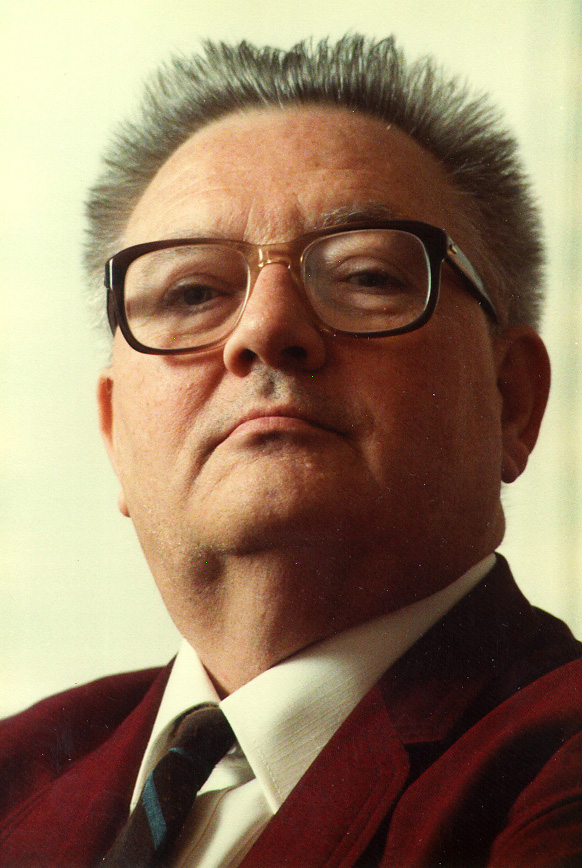
\includegraphics[scale=0.5]{ETJaynes2}
	\small

	Edwin Thompson Jaynes, circa 1982

	{\footnotesize (Public Domain, \url{https://en.wikipedia.org/w/index.php?curid=13019680}})
\end{figure}

\vfill

{
	\footnotesize
	The main body font used in this document is Cochineal, a fork of the Crimson fonts by Sebastian Koch, available on CTAN at \url{https://ctan.org/pkg/cochineal}.

	Mathematical typesetting uses the \texttt{newtxmath} package (\url{https://ctan.org/pkg/newtx}) with the \texttt{cochineal} option.

	Monospaced text (for URLs) uses the Inconsolata font through the \texttt{zi4} package\\
	(CTAN: \url{https://ctan.org/tex-archive/fonts/inconsolata-zi4}).

}

\end{document}